\documentclass[a4paper]{article}
\usepackage{student}
\usepackage{graphicx}
\usepackage{caption}
\usepackage[version=4]{mhchem}
\usepackage{tikz}
\usetikzlibrary{shapes.geometric, arrows.meta, positioning, decorations.pathreplacing}
\usepackage{enumitem}
\usepackage{tikz-3dplot}
\usepackage{multicol}
\usepackage{longtable}
\usepackage{amsmath}
\usepackage{booktabs}

\usepackage{url}

\tikzstyle{arrow} = [thick,->,>=stealth]

% Definindo o estilo de destaque com linhas pontilhadas
\tikzstyle{highlight} = [draw, dashed, thick, rectangle, rounded corners, inner sep=0.2cm, orange]


\tikzstyle{startstop} = [
rectangle, rounded corners, minimum width=0.5cm,
text centered, draw=black, fill=blue!10, font=\small
]
\tikzstyle{startstop_S} = [
rectangle, rounded corners, minimum width=0.5cm, minimum height=0.8cm,
text centered, draw=black, fill=green!30, font=\small
]
\tikzstyle{decision} = [
diamond, aspect=2, draw=black, fill=orange!15, align=center,
text centered, inner sep=0pt, font=\small
]
\tikzstyle{decision_S} = [
diamond, aspect=2, draw=black, fill=orange!30, align=center,
text centered, inner sep=0pt, font=\small
]
\tikzstyle{arrow} = [thick,->,>=stealth]



% Metadata
\date{\today}
\setmodule{PGF5261/IFUSP: Teoria de Grupos Aplicada a Sólidos e Moléculas. Prof.: Lucy Assali} 
\setterm{1o. semestre, 2025}

%-------------------------------%
% Other details
% TODO: Fill these
%-------------------------------%
\title{Exercício 02 - 22/04}
\setmembername{Nara Avila Moraes}  % Fill group member names
\setmemberuid{5716734}  % Fill group member uids (same order)

%-------------------------------%
% Add / Delete commands and packages
% TODO: Add / Delete here as you need
%-------------------------------%
\usepackage{amsmath,amssymb,bm}

\newcommand{\KL}{\mathrm{KL}}
\newcommand{\R}{\mathbb{R}}
\newcommand{\E}{\mathbb{E}}
\newcommand{\T}{\top}

\newcommand{\expdist}[2]{%
\normalfont{\textsc{Exp}}(#1, #2)%
}
\newcommand{\expparam}{\bm \lambda}
\newcommand{\Expparam}{\bm \Lambda}
\newcommand{\natparam}{\bm \eta}
\newcommand{\Natparam}{\bm H}
\newcommand{\sufstat}{\bm u}

% Main document
\begin{document}
% Add header
\header{}

\textbf{Questão 1.}
Considere as simetrias da molécula de etano eclipsado \ce{C2H6}, pertencente ao grupo $D_{3h}$ e responda os seguintes ítems:

\begin{center}
	\begin{minipage}{0.4\textwidth}
		\centering
		\includegraphics[width=0.6\textwidth]{figuras/etano_eclipsado.jpeg} 
		\captionof{figure}{Molécula do etano eclipsado}
	\end{minipage}
	\hfill
	\begin{minipage}{0.55\textwidth}
		\begin{itemize}
			\item[(1.1)] Identifique as operações de simetria da molécula.
			\item[(1.2)] Apresente a \textbf{tabela de multiplicação}.
			\item[(1.3)] Esse grupo é \textbf{cíclico}? Justifique.
			\item[(1.4)] O grupo é \textbf{abeliano}? Justifique.
			\item[(1.5)] Quais são as \textbf{classes} deste grupo?
			\item[(1.6)] Este grupo possui \textbf{subgrupos}?
		\end{itemize}
	\end{minipage}
\end{center}

\begin{answer}[Ítem 1.1 - Simetrias da Molécula]
\vspace{1em}

%%%%%%%%%%%%%%%%%%%%%%%%%%%%%%%%%%%%%%%%%%%%%%%%%%%%%%%%%%%%%%%%
%                              E
%%%%%%%%%%%%%%%%%%%%%%%%%%%%%%%%%%%%%%%%%%%%%%%%%%%%%%%%%%%%%%%%
\begin{itemize}[noitemsep, topsep=0pt, label=--]
        \begin{minipage}[t]{0.48\textwidth}
			      \centering
			      \includegraphics[width=5cm, height=5cm, keepaspectratio,clip]{figuras/E.png}
			      \captionof{figure}{Simetria \(E\)}
		      \end{minipage}
		      \hfill
		      \begin{minipage}[t]{0.48\textwidth}
			      \centering
			      \includegraphics[width=5cm, height=5cm, keepaspectratio,clip]{figuras/E.png}
			      \captionof{figure}{Operação \( E \) aplicada}
		      \end{minipage}
        \begin{align*}
        \textbf{:} \quad 
                E(1,2,3,4,5,6,7,8)                 & = (1,2,3,4,5,6,7,8) \\
        \end{align*}

%%%%%%%%%%%%%%%%%%%%%%%%%%%%%%%%%%%%%%%%%%%%%%%%%%%%%%%%%%%%%%%%
%                              C3
%%%%%%%%%%%%%%%%%%%%%%%%%%%%%%%%%%%%%%%%%%%%%%%%%%%%%%%%%%%%%%%%

        \begin{minipage}[t]{0.48\textwidth}
        \vspace{0.4em}
			      \centering
			      \includegraphics[width=5cm, height=5cm, keepaspectratio,clip]{figuras/C3.png}
			      \captionof{figure}{Eixo de rotação \(C_3\)}
		      \end{minipage}
		      \hfill
		      \begin{minipage}[t]{0.48\textwidth}
                      \vspace{0.4em}
			      \centering
			      \includegraphics[width=5cm, height=5cm, keepaspectratio,clip]{figuras/C3_1.png}
			      \captionof{figure}{Operação \( C_3 \) aplicada}
		      \end{minipage}
        \begin{align*}\textbf{:} \quad 
                C_3(1,2,3,4,5,6,7,8)               & = (1,2,5,3,4,8,6,7)  \\
                C_3^2(1,2,3,4,5,6,7,8)             & = 
                (1,2,4,5,3,7,8,6)\\
        \end{align*}

%%%%%%%%%%%%%%%%%%%%%%%%%%%%%%%%%%%%%%%%%%%%%%%%%%%%%%%%%%%%%%%%
%                              C2
%%%%%%%%%%%%%%%%%%%%%%%%%%%%%%%%%%%%%%%%%%%%%%%%%%%%%%%%%%%%%%%%
        \begin{minipage}[t]{0.48\textwidth}
			      \centering
			      \includegraphics[width=5cm, height=5cm, keepaspectratio,clip]{figuras/C2.png}
			      \captionof{figure}{Eixo de rotação \(C_2\)}
		      \end{minipage}
		      \hfill
		      \begin{minipage}[t]{0.48\textwidth}
			      \centering
			      \includegraphics[width=5cm, height=5cm, keepaspectratio,clip]{figuras/C2_1.png}
			      \captionof{figure}{Operação \( C_2^{(a)} \) aplicada}
		      \end{minipage}
              
        \begin{align*}\textbf{:} \quad 
            C_2^{(a)}(1,2,3,4,5,6,7,8)         & = 
            (2,1,6,8,7,3,5,4) \\
            C_2^{(b)}(1,2,3,4,5,6,7,8)         & =  
            (2,1,8,7,6,5,4,3)  \\
            C_2^{(c)}(1,2,3,4,5,6,7,8)         & = 
            (2,1,7,6,8,4,3,5) \\
        \end{align*}

%%%%%%%%%%%%%%%%%%%%%%%%%%%%%%%%%%%%%%%%%%%%%%%%%%%%%%%%%%%%%%%%
%                              sigma v
%%%%%%%%%%%%%%%%%%%%%%%%%%%%%%%%%%%%%%%%%%%%%%%%%%%%%%%%%%%%%%%%
        \begin{minipage}[t]{0.48\textwidth}
			      \centering
			      \includegraphics[width=5cm, height=5cm, keepaspectratio,clip]{figuras/sigma_v.png}
			      \captionof{figure}{Plano de reflexão \(\sigma_{v}\)}
		      \end{minipage}
		      \hfill
		      \begin{minipage}[t]{0.48\textwidth}
			      \centering
			      \includegraphics[width=5cm, height=5cm, keepaspectratio,clip]{figuras/sigma_v_1.png}
			      \captionof{figure}{Operação \(\sigma_{v1} \) aplicada}
		      \end{minipage}
        \begin{align*}\textbf{:} \quad 
            \sigma_{v1}(1,2,3,4,5,6,7,8)       & = 
            (1, 2, 4, 5, 3, 7, 8, 6) \\
            \sigma_{v2}(1,2,3,4,5,6,7,8)       & = 
            (1, 2, 5, 3, 4, 8, 6, 7) \\
            \sigma_{v3}(1,2,3,4,5,6,7,8)       & = 
            (1,2,4,3,5,7,6,8) \\
        \end{align*}
%%%%%%%%%%%%%%%%%%%%%%%%%%%%%%%%%%%%%%%%%%%%%%%%%%%%%%%%%%%%%%%%
%                              sigma h
%%%%%%%%%%%%%%%%%%%%%%%%%%%%%%%%%%%%%%%%%%%%%%%%%%%%%%%%%%%%%%%%
        \begin{minipage}[t]{0.48\textwidth}
			      \centering
			      \includegraphics[width=5cm, height=5cm, keepaspectratio,clip]{figuras/sigma_h.png}
			      \captionof{figure}{Plano de reflexão \(\sigma_{h}\)}
		      \end{minipage}
		      \hfill
		      \begin{minipage}[t]{0.48\textwidth}
			      \centering
			      \includegraphics[width=5cm, height=5cm, keepaspectratio,clip]{figuras/sigma_h_1.png}
			      \captionof{figure}{Operação \(\sigma_{h} \) aplicada}
		      \end{minipage}
              
        \begin{align*}\textbf{:} \quad 
                \sigma_h(1,2,3,4,5,6,7,8)          & = (2,1,6,7,8,3,4,5) \\
        \end{align*}

%%%%%%%%%%%%%%%%%%%%%%%%%%%%%%%%%%%%%%%%%%%%%%%%%%%%%%%%%%%%%%%%
%                              S_3
%%%%%%%%%%%%%%%%%%%%%%%%%%%%%%%%%%%%%%%%%%%%%%%%%%%%%%%%%%%%%%%%
        \begin{minipage}[t]{0.31\textwidth}
			      \centering
			      \includegraphics[width=5cm, height=5cm, keepaspectratio,clip]{figuras/C3.png}
			      \captionof{figure}{Eixo de rotação \(C_{3}\)}
		      \end{minipage}
		      \hfill
		      \begin{minipage}[t]{0.31\textwidth}
			      \centering
			      \includegraphics[width=5cm, height=5cm, keepaspectratio,clip]{figuras/C3_sigmah.png}
			      \captionof{figure}{Plano de reflexão \(\sigma_h \) }
		      \end{minipage}
              \begin{minipage}[t]{0.31\textwidth}
			      \centering
			      \includegraphics[width=5cm, height=5cm, keepaspectratio,clip]{figuras/S3_1.png}
			      \captionof{figure}{Operação \(S_{3} \) aplicada}
		      \end{minipage}
        \begin{align*}\textbf{:} \quad 
            S_3(1,2,3,4,5,6,7,8)               & = 
             (2,1,8,6,7,5,3,4)\\
            S_3^5(1,2,3,4,5,6,7,8)             & = (2,1,7,8,6,4,5,3)
        \end{align*}


	\end{itemize}
\end{answer}

\begin{answer}[Ítem 1.2 - Tabela de Multiplicação]
    % \input{operacoes_multiplicacao_01}
        % \begin{figure}
        %     \includegraphics[width=0.5\linewidth]{figuras/image.png}
        %     \caption{Enter Caption}
        %     \label{fig:enter-label}
        % \end{figure}
    Operações de Multiplicação:

\begin{longtable}{>{$}r<{$} >{$}r<{$} >{$}r<{$}}
\makebox[3.3cm][r]{$\mathrm{\mathrm{E}} \circ \mathrm{\mathrm{E}}$} &= $\mathrm{\mathrm{E}} \circ [1, 2, 3, 4, 5, 6, 7, 8]$ &= $[1, 2, 3, 4, 5, 6, 7, 8]$ &= \makebox[2.3cm][l]{$\mathrm{\mathrm{E}}$} \\
\makebox[3.3cm][r]{$\mathrm{\mathrm{E}} \circ \mathrm{\mathrm{C}_{3}}$} &= $\mathrm{\mathrm{E}} \circ [1, 2, 4, 5, 3, 7, 8, 6]$ &= $[1, 2, 4, 5, 3, 7, 8, 6]$ &= \makebox[2.3cm][l]{$\mathrm{\mathrm{C}_{3}}$} \\
\makebox[3.3cm][r]{$\mathrm{\mathrm{E}} \circ \mathrm{\mathrm{C}_{3}^{2}}$} &= $\mathrm{\mathrm{E}} \circ [1, 2, 5, 3, 4, 8, 6, 7]$ &= $[1, 2, 5, 3, 4, 8, 6, 7]$ &= \makebox[2.3cm][l]{$\mathrm{\mathrm{C}_{3}^{2}}$} \\
\makebox[3.3cm][r]{$\mathrm{\mathrm{E}} \circ \mathrm{\mathrm{C}_{2}^{(a)}}$} &= $\mathrm{\mathrm{E}} \circ [2, 1, 6, 8, 7, 3, 5, 4]$ &= $[2, 1, 6, 8, 7, 3, 5, 4]$ &= \makebox[2.3cm][l]{$\mathrm{\mathrm{C}_{2}^{(a)}}$} \\
\makebox[3.3cm][r]{$\mathrm{\mathrm{E}} \circ \mathrm{\mathrm{C}_{2}^{(b)}}$} &= $\mathrm{\mathrm{E}} \circ [2, 1, 8, 7, 6, 5, 4, 3]$ &= $[2, 1, 8, 7, 6, 5, 4, 3]$ &= \makebox[2.3cm][l]{$\mathrm{\mathrm{C}_{2}^{(b)}}$} \\
\makebox[3.3cm][r]{$\mathrm{\mathrm{E}} \circ \mathrm{\mathrm{C}_{2}^{(c)}}$} &= $\mathrm{\mathrm{E}} \circ [2, 1, 7, 6, 8, 4, 3, 5]$ &= $[2, 1, 7, 6, 8, 4, 3, 5]$ &= \makebox[2.3cm][l]{$\mathrm{\mathrm{C}_{2}^{(c)}}$} \\
\makebox[3.3cm][r]{$\mathrm{\mathrm{E}} \circ \mathrm{\sigma_{v1}}$} &= $\mathrm{\mathrm{E}} \circ [1, 2, 3, 5, 4, 6, 8, 7]$ &= $[1, 2, 3, 5, 4, 6, 8, 7]$ &= \makebox[2.3cm][l]{$\mathrm{\sigma_{v1}}$} \\
\makebox[3.3cm][r]{$\mathrm{\mathrm{E}} \circ \mathrm{\sigma_{v2}}$} &= $\mathrm{\mathrm{E}} \circ [1, 2, 5, 4, 3, 8, 7, 6]$ &= $[1, 2, 5, 4, 3, 8, 7, 6]$ &= \makebox[2.3cm][l]{$\mathrm{\sigma_{v2}}$} \\
\makebox[3.3cm][r]{$\mathrm{\mathrm{E}} \circ \mathrm{\sigma_{v3}}$} &= $\mathrm{\mathrm{E}} \circ [1, 2, 4, 3, 5, 7, 6, 8]$ &= $[1, 2, 4, 3, 5, 7, 6, 8]$ &= \makebox[2.3cm][l]{$\mathrm{\sigma_{v3}}$} \\
\makebox[3.3cm][r]{$\mathrm{\mathrm{E}} \circ \mathrm{\sigma_{h}}$} &= $\mathrm{\mathrm{E}} \circ [2, 1, 6, 7, 8, 3, 4, 5]$ &= $[2, 1, 6, 7, 8, 3, 4, 5]$ &= \makebox[2.3cm][l]{$\mathrm{\sigma_{h}}$} \\
\makebox[3.3cm][r]{$\mathrm{\mathrm{E}} \circ \mathrm{\mathrm{S}_{3}}$} &= $\mathrm{\mathrm{E}} \circ [2, 1, 7, 8, 6, 4, 5, 3]$ &= $[2, 1, 7, 8, 6, 4, 5, 3]$ &= \makebox[2.3cm][l]{$\mathrm{\mathrm{S}_{3}}$} \\
\makebox[3.3cm][r]{$\mathrm{\mathrm{E}} \circ \mathrm{\mathrm{S}_{3}^{5}}$} &= $\mathrm{\mathrm{E}} \circ [2, 1, 8, 6, 7, 5, 3, 4]$ &= $[2, 1, 8, 6, 7, 5, 3, 4]$ &= \makebox[2.3cm][l]{$\mathrm{\mathrm{S}_{3}^{5}}$} \\
\makebox[3.3cm][r]{$\mathrm{\mathrm{C}_{3}} \circ \mathrm{\mathrm{E}}$} &= $\mathrm{\mathrm{C}_{3}} \circ [1, 2, 3, 4, 5, 6, 7, 8]$ &= $[1, 2, 4, 5, 3, 7, 8, 6]$ &= \makebox[2.3cm][l]{$\mathrm{\mathrm{C}_{3}}$} \\
\makebox[3.3cm][r]{$\mathrm{\mathrm{C}_{3}} \circ \mathrm{\mathrm{C}_{3}}$} &= $\mathrm{\mathrm{C}_{3}} \circ [1, 2, 4, 5, 3, 7, 8, 6]$ &= $[1, 2, 5, 3, 4, 8, 6, 7]$ &= \makebox[2.3cm][l]{$\mathrm{\mathrm{C}_{3}^{2}}$} \\
\makebox[3.3cm][r]{$\mathrm{\mathrm{C}_{3}} \circ \mathrm{\mathrm{C}_{3}^{2}}$} &= $\mathrm{\mathrm{C}_{3}} \circ [1, 2, 5, 3, 4, 8, 6, 7]$ &= $[1, 2, 3, 4, 5, 6, 7, 8]$ &= \makebox[2.3cm][l]{$\mathrm{\mathrm{E}}$} \\
\makebox[3.3cm][r]{$\mathrm{\mathrm{C}_{3}} \circ \mathrm{\mathrm{C}_{2}^{(a)}}$} &= $\mathrm{\mathrm{C}_{3}} \circ [2, 1, 6, 8, 7, 3, 5, 4]$ &= $[2, 1, 8, 7, 6, 5, 4, 3]$ &= \makebox[2.3cm][l]{$\mathrm{\mathrm{C}_{2}^{(b)}}$} \\
\makebox[3.3cm][r]{$\mathrm{\mathrm{C}_{3}} \circ \mathrm{\mathrm{C}_{2}^{(b)}}$} &= $\mathrm{\mathrm{C}_{3}} \circ [2, 1, 8, 7, 6, 5, 4, 3]$ &= $[2, 1, 7, 6, 8, 4, 3, 5]$ &= \makebox[2.3cm][l]{$\mathrm{\mathrm{C}_{2}^{(c)}}$} \\
\makebox[3.3cm][r]{$\mathrm{\mathrm{C}_{3}} \circ \mathrm{\mathrm{C}_{2}^{(c)}}$} &= $\mathrm{\mathrm{C}_{3}} \circ [2, 1, 7, 6, 8, 4, 3, 5]$ &= $[2, 1, 6, 8, 7, 3, 5, 4]$ &= \makebox[2.3cm][l]{$\mathrm{\mathrm{C}_{2}^{(a)}}$} \\
\makebox[3.3cm][r]{$\mathrm{\mathrm{C}_{3}} \circ \mathrm{\sigma_{v1}}$} &= $\mathrm{\mathrm{C}_{3}} \circ [1, 2, 3, 5, 4, 6, 8, 7]$ &= $[1, 2, 5, 4, 3, 8, 7, 6]$ &= \makebox[2.3cm][l]{$\mathrm{\sigma_{v2}}$} \\
\makebox[3.3cm][r]{$\mathrm{\mathrm{C}_{3}} \circ \mathrm{\sigma_{v2}}$} &= $\mathrm{\mathrm{C}_{3}} \circ [1, 2, 5, 4, 3, 8, 7, 6]$ &= $[1, 2, 4, 3, 5, 7, 6, 8]$ &= \makebox[2.3cm][l]{$\mathrm{\sigma_{v3}}$} \\
\makebox[3.3cm][r]{$\mathrm{\mathrm{C}_{3}} \circ \mathrm{\sigma_{v3}}$} &= $\mathrm{\mathrm{C}_{3}} \circ [1, 2, 4, 3, 5, 7, 6, 8]$ &= $[1, 2, 3, 5, 4, 6, 8, 7]$ &= \makebox[2.3cm][l]{$\mathrm{\sigma_{v1}}$} \\
\makebox[3.3cm][r]{$\mathrm{\mathrm{C}_{3}} \circ \mathrm{\sigma_{h}}$} &= $\mathrm{\mathrm{C}_{3}} \circ [2, 1, 6, 7, 8, 3, 4, 5]$ &= $[2, 1, 7, 8, 6, 4, 5, 3]$ &= \makebox[2.3cm][l]{$\mathrm{\mathrm{S}_{3}}$} \\
\makebox[3.3cm][r]{$\mathrm{\mathrm{C}_{3}} \circ \mathrm{\mathrm{S}_{3}}$} &= $\mathrm{\mathrm{C}_{3}} \circ [2, 1, 7, 8, 6, 4, 5, 3]$ &= $[2, 1, 8, 6, 7, 5, 3, 4]$ &= \makebox[2.3cm][l]{$\mathrm{\mathrm{S}_{3}^{5}}$} \\
\makebox[3.3cm][r]{$\mathrm{\mathrm{C}_{3}} \circ \mathrm{\mathrm{S}_{3}^{5}}$} &= $\mathrm{\mathrm{C}_{3}} \circ [2, 1, 8, 6, 7, 5, 3, 4]$ &= $[2, 1, 6, 7, 8, 3, 4, 5]$ &= \makebox[2.3cm][l]{$\mathrm{\sigma_{h}}$} \\
\makebox[3.3cm][r]{$\mathrm{\mathrm{C}_{3}^{2}} \circ \mathrm{\mathrm{E}}$} &= $\mathrm{\mathrm{C}_{3}^{2}} \circ [1, 2, 3, 4, 5, 6, 7, 8]$ &= $[1, 2, 5, 3, 4, 8, 6, 7]$ &= \makebox[2.3cm][l]{$\mathrm{\mathrm{C}_{3}^{2}}$} \\
\makebox[3.3cm][r]{$\mathrm{\mathrm{C}_{3}^{2}} \circ \mathrm{\mathrm{C}_{3}}$} &= $\mathrm{\mathrm{C}_{3}^{2}} \circ [1, 2, 4, 5, 3, 7, 8, 6]$ &= $[1, 2, 3, 4, 5, 6, 7, 8]$ &= \makebox[2.3cm][l]{$\mathrm{\mathrm{E}}$} \\
\makebox[3.3cm][r]{$\mathrm{\mathrm{C}_{3}^{2}} \circ \mathrm{\mathrm{C}_{3}^{2}}$} &= $\mathrm{\mathrm{C}_{3}^{2}} \circ [1, 2, 5, 3, 4, 8, 6, 7]$ &= $[1, 2, 4, 5, 3, 7, 8, 6]$ &= \makebox[2.3cm][l]{$\mathrm{\mathrm{C}_{3}}$} \\
\makebox[3.3cm][r]{$\mathrm{\mathrm{C}_{3}^{2}} \circ \mathrm{\mathrm{C}_{2}^{(a)}}$} &= $\mathrm{\mathrm{C}_{3}^{2}} \circ [2, 1, 6, 8, 7, 3, 5, 4]$ &= $[2, 1, 7, 6, 8, 4, 3, 5]$ &= \makebox[2.3cm][l]{$\mathrm{\mathrm{C}_{2}^{(c)}}$} \\
\makebox[3.3cm][r]{$\mathrm{\mathrm{C}_{3}^{2}} \circ \mathrm{\mathrm{C}_{2}^{(b)}}$} &= $\mathrm{\mathrm{C}_{3}^{2}} \circ [2, 1, 8, 7, 6, 5, 4, 3]$ &= $[2, 1, 6, 8, 7, 3, 5, 4]$ &= \makebox[2.3cm][l]{$\mathrm{\mathrm{C}_{2}^{(a)}}$} \\
\makebox[3.3cm][r]{$\mathrm{\mathrm{C}_{3}^{2}} \circ \mathrm{\mathrm{C}_{2}^{(c)}}$} &= $\mathrm{\mathrm{C}_{3}^{2}} \circ [2, 1, 7, 6, 8, 4, 3, 5]$ &= $[2, 1, 8, 7, 6, 5, 4, 3]$ &= \makebox[2.3cm][l]{$\mathrm{\mathrm{C}_{2}^{(b)}}$} \\
\makebox[3.3cm][r]{$\mathrm{\mathrm{C}_{3}^{2}} \circ \mathrm{\sigma_{v1}}$} &= $\mathrm{\mathrm{C}_{3}^{2}} \circ [1, 2, 3, 5, 4, 6, 8, 7]$ &= $[1, 2, 4, 3, 5, 7, 6, 8]$ &= \makebox[2.3cm][l]{$\mathrm{\sigma_{v3}}$} \\
\makebox[3.3cm][r]{$\mathrm{\mathrm{C}_{3}^{2}} \circ \mathrm{\sigma_{v2}}$} &= $\mathrm{\mathrm{C}_{3}^{2}} \circ [1, 2, 5, 4, 3, 8, 7, 6]$ &= $[1, 2, 3, 5, 4, 6, 8, 7]$ &= \makebox[2.3cm][l]{$\mathrm{\sigma_{v1}}$} \\
\makebox[3.3cm][r]{$\mathrm{\mathrm{C}_{3}^{2}} \circ \mathrm{\sigma_{v3}}$} &= $\mathrm{\mathrm{C}_{3}^{2}} \circ [1, 2, 4, 3, 5, 7, 6, 8]$ &= $[1, 2, 5, 4, 3, 8, 7, 6]$ &= \makebox[2.3cm][l]{$\mathrm{\sigma_{v2}}$} \\
\makebox[3.3cm][r]{$\mathrm{\mathrm{C}_{3}^{2}} \circ \mathrm{\sigma_{h}}$} &= $\mathrm{\mathrm{C}_{3}^{2}} \circ [2, 1, 6, 7, 8, 3, 4, 5]$ &= $[2, 1, 8, 6, 7, 5, 3, 4]$ &= \makebox[2.3cm][l]{$\mathrm{\mathrm{S}_{3}^{5}}$} \\
\makebox[3.3cm][r]{$\mathrm{\mathrm{C}_{3}^{2}} \circ \mathrm{\mathrm{S}_{3}}$} &= $\mathrm{\mathrm{C}_{3}^{2}} \circ [2, 1, 7, 8, 6, 4, 5, 3]$ &= $[2, 1, 6, 7, 8, 3, 4, 5]$ &= \makebox[2.3cm][l]{$\mathrm{\sigma_{h}}$} \\
\makebox[3.3cm][r]{$\mathrm{\mathrm{C}_{3}^{2}} \circ \mathrm{\mathrm{S}_{3}^{5}}$} &= $\mathrm{\mathrm{C}_{3}^{2}} \circ [2, 1, 8, 6, 7, 5, 3, 4]$ &= $[2, 1, 7, 8, 6, 4, 5, 3]$ &= \makebox[2.3cm][l]{$\mathrm{\mathrm{S}_{3}}$} \\
\makebox[3.3cm][r]{$\mathrm{\mathrm{C}_{2}^{(a)}} \circ \mathrm{\mathrm{E}}$} &= $\mathrm{\mathrm{C}_{2}^{(a)}} \circ [1, 2, 3, 4, 5, 6, 7, 8]$ &= $[2, 1, 6, 8, 7, 3, 5, 4]$ &= \makebox[2.3cm][l]{$\mathrm{\mathrm{C}_{2}^{(a)}}$} \\
\makebox[3.3cm][r]{$\mathrm{\mathrm{C}_{2}^{(a)}} \circ \mathrm{\mathrm{C}_{3}}$} &= $\mathrm{\mathrm{C}_{2}^{(a)}} \circ [1, 2, 4, 5, 3, 7, 8, 6]$ &= $[2, 1, 7, 6, 8, 4, 3, 5]$ &= \makebox[2.3cm][l]{$\mathrm{\mathrm{C}_{2}^{(c)}}$} \\
\makebox[3.3cm][r]{$\mathrm{\mathrm{C}_{2}^{(a)}} \circ \mathrm{\mathrm{C}_{3}^{2}}$} &= $\mathrm{\mathrm{C}_{2}^{(a)}} \circ [1, 2, 5, 3, 4, 8, 6, 7]$ &= $[2, 1, 8, 7, 6, 5, 4, 3]$ &= \makebox[2.3cm][l]{$\mathrm{\mathrm{C}_{2}^{(b)}}$} \\
\makebox[3.3cm][r]{$\mathrm{\mathrm{C}_{2}^{(a)}} \circ \mathrm{\mathrm{C}_{2}^{(a)}}$} &= $\mathrm{\mathrm{C}_{2}^{(a)}} \circ [2, 1, 6, 8, 7, 3, 5, 4]$ &= $[1, 2, 3, 4, 5, 6, 7, 8]$ &= \makebox[2.3cm][l]{$\mathrm{\mathrm{E}}$} \\
\makebox[3.3cm][r]{$\mathrm{\mathrm{C}_{2}^{(a)}} \circ \mathrm{\mathrm{C}_{2}^{(b)}}$} &= $\mathrm{\mathrm{C}_{2}^{(a)}} \circ [2, 1, 8, 7, 6, 5, 4, 3]$ &= $[1, 2, 5, 3, 4, 8, 6, 7]$ &= \makebox[2.3cm][l]{$\mathrm{\mathrm{C}_{3}^{2}}$} \\
\makebox[3.3cm][r]{$\mathrm{\mathrm{C}_{2}^{(a)}} \circ \mathrm{\mathrm{C}_{2}^{(c)}}$} &= $\mathrm{\mathrm{C}_{2}^{(a)}} \circ [2, 1, 7, 6, 8, 4, 3, 5]$ &= $[1, 2, 4, 5, 3, 7, 8, 6]$ &= \makebox[2.3cm][l]{$\mathrm{\mathrm{C}_{3}}$} \\
\makebox[3.3cm][r]{$\mathrm{\mathrm{C}_{2}^{(a)}} \circ \mathrm{\sigma_{v1}}$} &= $\mathrm{\mathrm{C}_{2}^{(a)}} \circ [1, 2, 3, 5, 4, 6, 8, 7]$ &= $[2, 1, 6, 7, 8, 3, 4, 5]$ &= \makebox[2.3cm][l]{$\mathrm{\sigma_{h}}$} \\
\makebox[3.3cm][r]{$\mathrm{\mathrm{C}_{2}^{(a)}} \circ \mathrm{\sigma_{v2}}$} &= $\mathrm{\mathrm{C}_{2}^{(a)}} \circ [1, 2, 5, 4, 3, 8, 7, 6]$ &= $[2, 1, 8, 6, 7, 5, 3, 4]$ &= \makebox[2.3cm][l]{$\mathrm{\mathrm{S}_{3}^{5}}$} \\
\makebox[3.3cm][r]{$\mathrm{\mathrm{C}_{2}^{(a)}} \circ \mathrm{\sigma_{v3}}$} &= $\mathrm{\mathrm{C}_{2}^{(a)}} \circ [1, 2, 4, 3, 5, 7, 6, 8]$ &= $[2, 1, 7, 8, 6, 4, 5, 3]$ &= \makebox[2.3cm][l]{$\mathrm{\mathrm{S}_{3}}$} \\
\makebox[3.3cm][r]{$\mathrm{\mathrm{C}_{2}^{(a)}} \circ \mathrm{\sigma_{h}}$} &= $\mathrm{\mathrm{C}_{2}^{(a)}} \circ [2, 1, 6, 7, 8, 3, 4, 5]$ &= $[1, 2, 3, 5, 4, 6, 8, 7]$ &= \makebox[2.3cm][l]{$\mathrm{\sigma_{v1}}$} \\
\makebox[3.3cm][r]{$\mathrm{\mathrm{C}_{2}^{(a)}} \circ \mathrm{\mathrm{S}_{3}}$} &= $\mathrm{\mathrm{C}_{2}^{(a)}} \circ [2, 1, 7, 8, 6, 4, 5, 3]$ &= $[1, 2, 4, 3, 5, 7, 6, 8]$ &= \makebox[2.3cm][l]{$\mathrm{\sigma_{v3}}$} \\
\makebox[3.3cm][r]{$\mathrm{\mathrm{C}_{2}^{(a)}} \circ \mathrm{\mathrm{S}_{3}^{5}}$} &= $\mathrm{\mathrm{C}_{2}^{(a)}} \circ [2, 1, 8, 6, 7, 5, 3, 4]$ &= $[1, 2, 5, 4, 3, 8, 7, 6]$ &= \makebox[2.3cm][l]{$\mathrm{\sigma_{v2}}$} \\
\makebox[3.3cm][r]{$\mathrm{\mathrm{C}_{2}^{(b)}} \circ \mathrm{\mathrm{E}}$} &= $\mathrm{\mathrm{C}_{2}^{(b)}} \circ [1, 2, 3, 4, 5, 6, 7, 8]$ &= $[2, 1, 8, 7, 6, 5, 4, 3]$ &= \makebox[2.3cm][l]{$\mathrm{\mathrm{C}_{2}^{(b)}}$} \\
\makebox[3.3cm][r]{$\mathrm{\mathrm{C}_{2}^{(b)}} \circ \mathrm{\mathrm{C}_{3}}$} &= $\mathrm{\mathrm{C}_{2}^{(b)}} \circ [1, 2, 4, 5, 3, 7, 8, 6]$ &= $[2, 1, 6, 8, 7, 3, 5, 4]$ &= \makebox[2.3cm][l]{$\mathrm{\mathrm{C}_{2}^{(a)}}$} \\
\makebox[3.3cm][r]{$\mathrm{\mathrm{C}_{2}^{(b)}} \circ \mathrm{\mathrm{C}_{3}^{2}}$} &= $\mathrm{\mathrm{C}_{2}^{(b)}} \circ [1, 2, 5, 3, 4, 8, 6, 7]$ &= $[2, 1, 7, 6, 8, 4, 3, 5]$ &= \makebox[2.3cm][l]{$\mathrm{\mathrm{C}_{2}^{(c)}}$} \\
\makebox[3.3cm][r]{$\mathrm{\mathrm{C}_{2}^{(b)}} \circ \mathrm{\mathrm{C}_{2}^{(a)}}$} &= $\mathrm{\mathrm{C}_{2}^{(b)}} \circ [2, 1, 6, 8, 7, 3, 5, 4]$ &= $[1, 2, 4, 5, 3, 7, 8, 6]$ &= \makebox[2.3cm][l]{$\mathrm{\mathrm{C}_{3}}$} \\
\makebox[3.3cm][r]{$\mathrm{\mathrm{C}_{2}^{(b)}} \circ \mathrm{\mathrm{C}_{2}^{(b)}}$} &= $\mathrm{\mathrm{C}_{2}^{(b)}} \circ [2, 1, 8, 7, 6, 5, 4, 3]$ &= $[1, 2, 3, 4, 5, 6, 7, 8]$ &= \makebox[2.3cm][l]{$\mathrm{\mathrm{E}}$} \\
\makebox[3.3cm][r]{$\mathrm{\mathrm{C}_{2}^{(b)}} \circ \mathrm{\mathrm{C}_{2}^{(c)}}$} &= $\mathrm{\mathrm{C}_{2}^{(b)}} \circ [2, 1, 7, 6, 8, 4, 3, 5]$ &= $[1, 2, 5, 3, 4, 8, 6, 7]$ &= \makebox[2.3cm][l]{$\mathrm{\mathrm{C}_{3}^{2}}$} \\
\makebox[3.3cm][r]{$\mathrm{\mathrm{C}_{2}^{(b)}} \circ \mathrm{\sigma_{v1}}$} &= $\mathrm{\mathrm{C}_{2}^{(b)}} \circ [1, 2, 3, 5, 4, 6, 8, 7]$ &= $[2, 1, 7, 8, 6, 4, 5, 3]$ &= \makebox[2.3cm][l]{$\mathrm{\mathrm{S}_{3}}$} \\
\makebox[3.3cm][r]{$\mathrm{\mathrm{C}_{2}^{(b)}} \circ \mathrm{\sigma_{v2}}$} &= $\mathrm{\mathrm{C}_{2}^{(b)}} \circ [1, 2, 5, 4, 3, 8, 7, 6]$ &= $[2, 1, 6, 7, 8, 3, 4, 5]$ &= \makebox[2.3cm][l]{$\mathrm{\sigma_{h}}$} \\
\makebox[3.3cm][r]{$\mathrm{\mathrm{C}_{2}^{(b)}} \circ \mathrm{\sigma_{v3}}$} &= $\mathrm{\mathrm{C}_{2}^{(b)}} \circ [1, 2, 4, 3, 5, 7, 6, 8]$ &= $[2, 1, 8, 6, 7, 5, 3, 4]$ &= \makebox[2.3cm][l]{$\mathrm{\mathrm{S}_{3}^{5}}$} \\
\makebox[3.3cm][r]{$\mathrm{\mathrm{C}_{2}^{(b)}} \circ \mathrm{\sigma_{h}}$} &= $\mathrm{\mathrm{C}_{2}^{(b)}} \circ [2, 1, 6, 7, 8, 3, 4, 5]$ &= $[1, 2, 5, 4, 3, 8, 7, 6]$ &= \makebox[2.3cm][l]{$\mathrm{\sigma_{v2}}$} \\
\makebox[3.3cm][r]{$\mathrm{\mathrm{C}_{2}^{(b)}} \circ \mathrm{\mathrm{S}_{3}}$} &= $\mathrm{\mathrm{C}_{2}^{(b)}} \circ [2, 1, 7, 8, 6, 4, 5, 3]$ &= $[1, 2, 3, 5, 4, 6, 8, 7]$ &= \makebox[2.3cm][l]{$\mathrm{\sigma_{v1}}$} \\
\makebox[3.3cm][r]{$\mathrm{\mathrm{C}_{2}^{(b)}} \circ \mathrm{\mathrm{S}_{3}^{5}}$} &= $\mathrm{\mathrm{C}_{2}^{(b)}} \circ [2, 1, 8, 6, 7, 5, 3, 4]$ &= $[1, 2, 4, 3, 5, 7, 6, 8]$ &= \makebox[2.3cm][l]{$\mathrm{\sigma_{v3}}$} \\
\makebox[3.3cm][r]{$\mathrm{\mathrm{C}_{2}^{(c)}} \circ \mathrm{\mathrm{E}}$} &= $\mathrm{\mathrm{C}_{2}^{(c)}} \circ [1, 2, 3, 4, 5, 6, 7, 8]$ &= $[2, 1, 7, 6, 8, 4, 3, 5]$ &= \makebox[2.3cm][l]{$\mathrm{\mathrm{C}_{2}^{(c)}}$} \\
\makebox[3.3cm][r]{$\mathrm{\mathrm{C}_{2}^{(c)}} \circ \mathrm{\mathrm{C}_{3}}$} &= $\mathrm{\mathrm{C}_{2}^{(c)}} \circ [1, 2, 4, 5, 3, 7, 8, 6]$ &= $[2, 1, 8, 7, 6, 5, 4, 3]$ &= \makebox[2.3cm][l]{$\mathrm{\mathrm{C}_{2}^{(b)}}$} \\
\makebox[3.3cm][r]{$\mathrm{\mathrm{C}_{2}^{(c)}} \circ \mathrm{\mathrm{C}_{3}^{2}}$} &= $\mathrm{\mathrm{C}_{2}^{(c)}} \circ [1, 2, 5, 3, 4, 8, 6, 7]$ &= $[2, 1, 6, 8, 7, 3, 5, 4]$ &= \makebox[2.3cm][l]{$\mathrm{\mathrm{C}_{2}^{(a)}}$} \\
\makebox[3.3cm][r]{$\mathrm{\mathrm{C}_{2}^{(c)}} \circ \mathrm{\mathrm{C}_{2}^{(a)}}$} &= $\mathrm{\mathrm{C}_{2}^{(c)}} \circ [2, 1, 6, 8, 7, 3, 5, 4]$ &= $[1, 2, 5, 3, 4, 8, 6, 7]$ &= \makebox[2.3cm][l]{$\mathrm{\mathrm{C}_{3}^{2}}$} \\
\makebox[3.3cm][r]{$\mathrm{\mathrm{C}_{2}^{(c)}} \circ \mathrm{\mathrm{C}_{2}^{(b)}}$} &= $\mathrm{\mathrm{C}_{2}^{(c)}} \circ [2, 1, 8, 7, 6, 5, 4, 3]$ &= $[1, 2, 4, 5, 3, 7, 8, 6]$ &= \makebox[2.3cm][l]{$\mathrm{\mathrm{C}_{3}}$} \\
\makebox[3.3cm][r]{$\mathrm{\mathrm{C}_{2}^{(c)}} \circ \mathrm{\mathrm{C}_{2}^{(c)}}$} &= $\mathrm{\mathrm{C}_{2}^{(c)}} \circ [2, 1, 7, 6, 8, 4, 3, 5]$ &= $[1, 2, 3, 4, 5, 6, 7, 8]$ &= \makebox[2.3cm][l]{$\mathrm{\mathrm{E}}$} \\
\makebox[3.3cm][r]{$\mathrm{\mathrm{C}_{2}^{(c)}} \circ \mathrm{\sigma_{v1}}$} &= $\mathrm{\mathrm{C}_{2}^{(c)}} \circ [1, 2, 3, 5, 4, 6, 8, 7]$ &= $[2, 1, 8, 6, 7, 5, 3, 4]$ &= \makebox[2.3cm][l]{$\mathrm{\mathrm{S}_{3}^{5}}$} \\
\makebox[3.3cm][r]{$\mathrm{\mathrm{C}_{2}^{(c)}} \circ \mathrm{\sigma_{v2}}$} &= $\mathrm{\mathrm{C}_{2}^{(c)}} \circ [1, 2, 5, 4, 3, 8, 7, 6]$ &= $[2, 1, 7, 8, 6, 4, 5, 3]$ &= \makebox[2.3cm][l]{$\mathrm{\mathrm{S}_{3}}$} \\
\makebox[3.3cm][r]{$\mathrm{\mathrm{C}_{2}^{(c)}} \circ \mathrm{\sigma_{v3}}$} &= $\mathrm{\mathrm{C}_{2}^{(c)}} \circ [1, 2, 4, 3, 5, 7, 6, 8]$ &= $[2, 1, 6, 7, 8, 3, 4, 5]$ &= \makebox[2.3cm][l]{$\mathrm{\sigma_{h}}$} \\
\makebox[3.3cm][r]{$\mathrm{\mathrm{C}_{2}^{(c)}} \circ \mathrm{\sigma_{h}}$} &= $\mathrm{\mathrm{C}_{2}^{(c)}} \circ [2, 1, 6, 7, 8, 3, 4, 5]$ &= $[1, 2, 4, 3, 5, 7, 6, 8]$ &= \makebox[2.3cm][l]{$\mathrm{\sigma_{v3}}$} \\
\makebox[3.3cm][r]{$\mathrm{\mathrm{C}_{2}^{(c)}} \circ \mathrm{\mathrm{S}_{3}}$} &= $\mathrm{\mathrm{C}_{2}^{(c)}} \circ [2, 1, 7, 8, 6, 4, 5, 3]$ &= $[1, 2, 5, 4, 3, 8, 7, 6]$ &= \makebox[2.3cm][l]{$\mathrm{\sigma_{v2}}$} \\
\makebox[3.3cm][r]{$\mathrm{\mathrm{C}_{2}^{(c)}} \circ \mathrm{\mathrm{S}_{3}^{5}}$} &= $\mathrm{\mathrm{C}_{2}^{(c)}} \circ [2, 1, 8, 6, 7, 5, 3, 4]$ &= $[1, 2, 3, 5, 4, 6, 8, 7]$ &= \makebox[2.3cm][l]{$\mathrm{\sigma_{v1}}$} \\
\makebox[3.3cm][r]{$\mathrm{\sigma_{v1}} \circ \mathrm{\mathrm{E}}$} &= $\mathrm{\sigma_{v1}} \circ [1, 2, 3, 4, 5, 6, 7, 8]$ &= $[1, 2, 3, 5, 4, 6, 8, 7]$ &= \makebox[2.3cm][l]{$\mathrm{\sigma_{v1}}$} \\
\makebox[3.3cm][r]{$\mathrm{\sigma_{v1}} \circ \mathrm{\mathrm{C}_{3}}$} &= $\mathrm{\sigma_{v1}} \circ [1, 2, 4, 5, 3, 7, 8, 6]$ &= $[1, 2, 4, 3, 5, 7, 6, 8]$ &= \makebox[2.3cm][l]{$\mathrm{\sigma_{v3}}$} \\
\makebox[3.3cm][r]{$\mathrm{\sigma_{v1}} \circ \mathrm{\mathrm{C}_{3}^{2}}$} &= $\mathrm{\sigma_{v1}} \circ [1, 2, 5, 3, 4, 8, 6, 7]$ &= $[1, 2, 5, 4, 3, 8, 7, 6]$ &= \makebox[2.3cm][l]{$\mathrm{\sigma_{v2}}$} \\
\makebox[3.3cm][r]{$\mathrm{\sigma_{v1}} \circ \mathrm{\mathrm{C}_{2}^{(a)}}$} &= $\mathrm{\sigma_{v1}} \circ [2, 1, 6, 8, 7, 3, 5, 4]$ &= $[2, 1, 6, 7, 8, 3, 4, 5]$ &= \makebox[2.3cm][l]{$\mathrm{\sigma_{h}}$} \\
\makebox[3.3cm][r]{$\mathrm{\sigma_{v1}} \circ \mathrm{\mathrm{C}_{2}^{(b)}}$} &= $\mathrm{\sigma_{v1}} \circ [2, 1, 8, 7, 6, 5, 4, 3]$ &= $[2, 1, 8, 6, 7, 5, 3, 4]$ &= \makebox[2.3cm][l]{$\mathrm{\mathrm{S}_{3}^{5}}$} \\
\makebox[3.3cm][r]{$\mathrm{\sigma_{v1}} \circ \mathrm{\mathrm{C}_{2}^{(c)}}$} &= $\mathrm{\sigma_{v1}} \circ [2, 1, 7, 6, 8, 4, 3, 5]$ &= $[2, 1, 7, 8, 6, 4, 5, 3]$ &= \makebox[2.3cm][l]{$\mathrm{\mathrm{S}_{3}}$} \\
\makebox[3.3cm][r]{$\mathrm{\sigma_{v1}} \circ \mathrm{\sigma_{v1}}$} &= $\mathrm{\sigma_{v1}} \circ [1, 2, 3, 5, 4, 6, 8, 7]$ &= $[1, 2, 3, 4, 5, 6, 7, 8]$ &= \makebox[2.3cm][l]{$\mathrm{\mathrm{E}}$} \\
\makebox[3.3cm][r]{$\mathrm{\sigma_{v1}} \circ \mathrm{\sigma_{v2}}$} &= $\mathrm{\sigma_{v1}} \circ [1, 2, 5, 4, 3, 8, 7, 6]$ &= $[1, 2, 5, 3, 4, 8, 6, 7]$ &= \makebox[2.3cm][l]{$\mathrm{\mathrm{C}_{3}^{2}}$} \\
\makebox[3.3cm][r]{$\mathrm{\sigma_{v1}} \circ \mathrm{\sigma_{v3}}$} &= $\mathrm{\sigma_{v1}} \circ [1, 2, 4, 3, 5, 7, 6, 8]$ &= $[1, 2, 4, 5, 3, 7, 8, 6]$ &= \makebox[2.3cm][l]{$\mathrm{\mathrm{C}_{3}}$} \\
\makebox[3.3cm][r]{$\mathrm{\sigma_{v1}} \circ \mathrm{\sigma_{h}}$} &= $\mathrm{\sigma_{v1}} \circ [2, 1, 6, 7, 8, 3, 4, 5]$ &= $[2, 1, 6, 8, 7, 3, 5, 4]$ &= \makebox[2.3cm][l]{$\mathrm{\mathrm{C}_{2}^{(a)}}$} \\
\makebox[3.3cm][r]{$\mathrm{\sigma_{v1}} \circ \mathrm{\mathrm{S}_{3}}$} &= $\mathrm{\sigma_{v1}} \circ [2, 1, 7, 8, 6, 4, 5, 3]$ &= $[2, 1, 7, 6, 8, 4, 3, 5]$ &= \makebox[2.3cm][l]{$\mathrm{\mathrm{C}_{2}^{(c)}}$} \\
\makebox[3.3cm][r]{$\mathrm{\sigma_{v1}} \circ \mathrm{\mathrm{S}_{3}^{5}}$} &= $\mathrm{\sigma_{v1}} \circ [2, 1, 8, 6, 7, 5, 3, 4]$ &= $[2, 1, 8, 7, 6, 5, 4, 3]$ &= \makebox[2.3cm][l]{$\mathrm{\mathrm{C}_{2}^{(b)}}$} \\
\makebox[3.3cm][r]{$\mathrm{\sigma_{v2}} \circ \mathrm{\mathrm{E}}$} &= $\mathrm{\sigma_{v2}} \circ [1, 2, 3, 4, 5, 6, 7, 8]$ &= $[1, 2, 5, 4, 3, 8, 7, 6]$ &= \makebox[2.3cm][l]{$\mathrm{\sigma_{v2}}$} \\
\makebox[3.3cm][r]{$\mathrm{\sigma_{v2}} \circ \mathrm{\mathrm{C}_{3}}$} &= $\mathrm{\sigma_{v2}} \circ [1, 2, 4, 5, 3, 7, 8, 6]$ &= $[1, 2, 3, 5, 4, 6, 8, 7]$ &= \makebox[2.3cm][l]{$\mathrm{\sigma_{v1}}$} \\
\makebox[3.3cm][r]{$\mathrm{\sigma_{v2}} \circ \mathrm{\mathrm{C}_{3}^{2}}$} &= $\mathrm{\sigma_{v2}} \circ [1, 2, 5, 3, 4, 8, 6, 7]$ &= $[1, 2, 4, 3, 5, 7, 6, 8]$ &= \makebox[2.3cm][l]{$\mathrm{\sigma_{v3}}$} \\
\makebox[3.3cm][r]{$\mathrm{\sigma_{v2}} \circ \mathrm{\mathrm{C}_{2}^{(a)}}$} &= $\mathrm{\sigma_{v2}} \circ [2, 1, 6, 8, 7, 3, 5, 4]$ &= $[2, 1, 7, 8, 6, 4, 5, 3]$ &= \makebox[2.3cm][l]{$\mathrm{\mathrm{S}_{3}}$} \\
\makebox[3.3cm][r]{$\mathrm{\sigma_{v2}} \circ \mathrm{\mathrm{C}_{2}^{(b)}}$} &= $\mathrm{\sigma_{v2}} \circ [2, 1, 8, 7, 6, 5, 4, 3]$ &= $[2, 1, 6, 7, 8, 3, 4, 5]$ &= \makebox[2.3cm][l]{$\mathrm{\sigma_{h}}$} \\
\makebox[3.3cm][r]{$\mathrm{\sigma_{v2}} \circ \mathrm{\mathrm{C}_{2}^{(c)}}$} &= $\mathrm{\sigma_{v2}} \circ [2, 1, 7, 6, 8, 4, 3, 5]$ &= $[2, 1, 8, 6, 7, 5, 3, 4]$ &= \makebox[2.3cm][l]{$\mathrm{\mathrm{S}_{3}^{5}}$} \\
\makebox[3.3cm][r]{$\mathrm{\sigma_{v2}} \circ \mathrm{\sigma_{v1}}$} &= $\mathrm{\sigma_{v2}} \circ [1, 2, 3, 5, 4, 6, 8, 7]$ &= $[1, 2, 4, 5, 3, 7, 8, 6]$ &= \makebox[2.3cm][l]{$\mathrm{\mathrm{C}_{3}}$} \\
\makebox[3.3cm][r]{$\mathrm{\sigma_{v2}} \circ \mathrm{\sigma_{v2}}$} &= $\mathrm{\sigma_{v2}} \circ [1, 2, 5, 4, 3, 8, 7, 6]$ &= $[1, 2, 3, 4, 5, 6, 7, 8]$ &= \makebox[2.3cm][l]{$\mathrm{\mathrm{E}}$} \\
\makebox[3.3cm][r]{$\mathrm{\sigma_{v2}} \circ \mathrm{\sigma_{v3}}$} &= $\mathrm{\sigma_{v2}} \circ [1, 2, 4, 3, 5, 7, 6, 8]$ &= $[1, 2, 5, 3, 4, 8, 6, 7]$ &= \makebox[2.3cm][l]{$\mathrm{\mathrm{C}_{3}^{2}}$} \\
\makebox[3.3cm][r]{$\mathrm{\sigma_{v2}} \circ \mathrm{\sigma_{h}}$} &= $\mathrm{\sigma_{v2}} \circ [2, 1, 6, 7, 8, 3, 4, 5]$ &= $[2, 1, 8, 7, 6, 5, 4, 3]$ &= \makebox[2.3cm][l]{$\mathrm{\mathrm{C}_{2}^{(b)}}$} \\
\makebox[3.3cm][r]{$\mathrm{\sigma_{v2}} \circ \mathrm{\mathrm{S}_{3}}$} &= $\mathrm{\sigma_{v2}} \circ [2, 1, 7, 8, 6, 4, 5, 3]$ &= $[2, 1, 6, 8, 7, 3, 5, 4]$ &= \makebox[2.3cm][l]{$\mathrm{\mathrm{C}_{2}^{(a)}}$} \\
\makebox[3.3cm][r]{$\mathrm{\sigma_{v2}} \circ \mathrm{\mathrm{S}_{3}^{5}}$} &= $\mathrm{\sigma_{v2}} \circ [2, 1, 8, 6, 7, 5, 3, 4]$ &= $[2, 1, 7, 6, 8, 4, 3, 5]$ &= \makebox[2.3cm][l]{$\mathrm{\mathrm{C}_{2}^{(c)}}$} \\
\makebox[3.3cm][r]{$\mathrm{\sigma_{v3}} \circ \mathrm{\mathrm{E}}$} &= $\mathrm{\sigma_{v3}} \circ [1, 2, 3, 4, 5, 6, 7, 8]$ &= $[1, 2, 4, 3, 5, 7, 6, 8]$ &= \makebox[2.3cm][l]{$\mathrm{\sigma_{v3}}$} \\
\makebox[3.3cm][r]{$\mathrm{\sigma_{v3}} \circ \mathrm{\mathrm{C}_{3}}$} &= $\mathrm{\sigma_{v3}} \circ [1, 2, 4, 5, 3, 7, 8, 6]$ &= $[1, 2, 5, 4, 3, 8, 7, 6]$ &= \makebox[2.3cm][l]{$\mathrm{\sigma_{v2}}$} \\
\makebox[3.3cm][r]{$\mathrm{\sigma_{v3}} \circ \mathrm{\mathrm{C}_{3}^{2}}$} &= $\mathrm{\sigma_{v3}} \circ [1, 2, 5, 3, 4, 8, 6, 7]$ &= $[1, 2, 3, 5, 4, 6, 8, 7]$ &= \makebox[2.3cm][l]{$\mathrm{\sigma_{v1}}$} \\
\makebox[3.3cm][r]{$\mathrm{\sigma_{v3}} \circ \mathrm{\mathrm{C}_{2}^{(a)}}$} &= $\mathrm{\sigma_{v3}} \circ [2, 1, 6, 8, 7, 3, 5, 4]$ &= $[2, 1, 8, 6, 7, 5, 3, 4]$ &= \makebox[2.3cm][l]{$\mathrm{\mathrm{S}_{3}^{5}}$} \\
\makebox[3.3cm][r]{$\mathrm{\sigma_{v3}} \circ \mathrm{\mathrm{C}_{2}^{(b)}}$} &= $\mathrm{\sigma_{v3}} \circ [2, 1, 8, 7, 6, 5, 4, 3]$ &= $[2, 1, 7, 8, 6, 4, 5, 3]$ &= \makebox[2.3cm][l]{$\mathrm{\mathrm{S}_{3}}$} \\
\makebox[3.3cm][r]{$\mathrm{\sigma_{v3}} \circ \mathrm{\mathrm{C}_{2}^{(c)}}$} &= $\mathrm{\sigma_{v3}} \circ [2, 1, 7, 6, 8, 4, 3, 5]$ &= $[2, 1, 6, 7, 8, 3, 4, 5]$ &= \makebox[2.3cm][l]{$\mathrm{\sigma_{h}}$} \\
\makebox[3.3cm][r]{$\mathrm{\sigma_{v3}} \circ \mathrm{\sigma_{v1}}$} &= $\mathrm{\sigma_{v3}} \circ [1, 2, 3, 5, 4, 6, 8, 7]$ &= $[1, 2, 5, 3, 4, 8, 6, 7]$ &= \makebox[2.3cm][l]{$\mathrm{\mathrm{C}_{3}^{2}}$} \\
\makebox[3.3cm][r]{$\mathrm{\sigma_{v3}} \circ \mathrm{\sigma_{v2}}$} &= $\mathrm{\sigma_{v3}} \circ [1, 2, 5, 4, 3, 8, 7, 6]$ &= $[1, 2, 4, 5, 3, 7, 8, 6]$ &= \makebox[2.3cm][l]{$\mathrm{\mathrm{C}_{3}}$} \\
\makebox[3.3cm][r]{$\mathrm{\sigma_{v3}} \circ \mathrm{\sigma_{v3}}$} &= $\mathrm{\sigma_{v3}} \circ [1, 2, 4, 3, 5, 7, 6, 8]$ &= $[1, 2, 3, 4, 5, 6, 7, 8]$ &= \makebox[2.3cm][l]{$\mathrm{\mathrm{E}}$} \\
\makebox[3.3cm][r]{$\mathrm{\sigma_{v3}} \circ \mathrm{\sigma_{h}}$} &= $\mathrm{\sigma_{v3}} \circ [2, 1, 6, 7, 8, 3, 4, 5]$ &= $[2, 1, 7, 6, 8, 4, 3, 5]$ &= \makebox[2.3cm][l]{$\mathrm{\mathrm{C}_{2}^{(c)}}$} \\
\makebox[3.3cm][r]{$\mathrm{\sigma_{v3}} \circ \mathrm{\mathrm{S}_{3}}$} &= $\mathrm{\sigma_{v3}} \circ [2, 1, 7, 8, 6, 4, 5, 3]$ &= $[2, 1, 8, 7, 6, 5, 4, 3]$ &= \makebox[2.3cm][l]{$\mathrm{\mathrm{C}_{2}^{(b)}}$} \\
\makebox[3.3cm][r]{$\mathrm{\sigma_{v3}} \circ \mathrm{\mathrm{S}_{3}^{5}}$} &= $\mathrm{\sigma_{v3}} \circ [2, 1, 8, 6, 7, 5, 3, 4]$ &= $[2, 1, 6, 8, 7, 3, 5, 4]$ &= \makebox[2.3cm][l]{$\mathrm{\mathrm{C}_{2}^{(a)}}$} \\
\makebox[3.3cm][r]{$\mathrm{\sigma_{h}} \circ \mathrm{\mathrm{E}}$} &= $\mathrm{\sigma_{h}} \circ [1, 2, 3, 4, 5, 6, 7, 8]$ &= $[2, 1, 6, 7, 8, 3, 4, 5]$ &= \makebox[2.3cm][l]{$\mathrm{\sigma_{h}}$} \\
\makebox[3.3cm][r]{$\mathrm{\sigma_{h}} \circ \mathrm{\mathrm{C}_{3}}$} &= $\mathrm{\sigma_{h}} \circ [1, 2, 4, 5, 3, 7, 8, 6]$ &= $[2, 1, 7, 8, 6, 4, 5, 3]$ &= \makebox[2.3cm][l]{$\mathrm{\mathrm{S}_{3}}$} \\
\makebox[3.3cm][r]{$\mathrm{\sigma_{h}} \circ \mathrm{\mathrm{C}_{3}^{2}}$} &= $\mathrm{\sigma_{h}} \circ [1, 2, 5, 3, 4, 8, 6, 7]$ &= $[2, 1, 8, 6, 7, 5, 3, 4]$ &= \makebox[2.3cm][l]{$\mathrm{\mathrm{S}_{3}^{5}}$} \\
\makebox[3.3cm][r]{$\mathrm{\sigma_{h}} \circ \mathrm{\mathrm{C}_{2}^{(a)}}$} &= $\mathrm{\sigma_{h}} \circ [2, 1, 6, 8, 7, 3, 5, 4]$ &= $[1, 2, 3, 5, 4, 6, 8, 7]$ &= \makebox[2.3cm][l]{$\mathrm{\sigma_{v1}}$} \\
\makebox[3.3cm][r]{$\mathrm{\sigma_{h}} \circ \mathrm{\mathrm{C}_{2}^{(b)}}$} &= $\mathrm{\sigma_{h}} \circ [2, 1, 8, 7, 6, 5, 4, 3]$ &= $[1, 2, 5, 4, 3, 8, 7, 6]$ &= \makebox[2.3cm][l]{$\mathrm{\sigma_{v2}}$} \\
\makebox[3.3cm][r]{$\mathrm{\sigma_{h}} \circ \mathrm{\mathrm{C}_{2}^{(c)}}$} &= $\mathrm{\sigma_{h}} \circ [2, 1, 7, 6, 8, 4, 3, 5]$ &= $[1, 2, 4, 3, 5, 7, 6, 8]$ &= \makebox[2.3cm][l]{$\mathrm{\sigma_{v3}}$} \\
\makebox[3.3cm][r]{$\mathrm{\sigma_{h}} \circ \mathrm{\sigma_{v1}}$} &= $\mathrm{\sigma_{h}} \circ [1, 2, 3, 5, 4, 6, 8, 7]$ &= $[2, 1, 6, 8, 7, 3, 5, 4]$ &= \makebox[2.3cm][l]{$\mathrm{\mathrm{C}_{2}^{(a)}}$} \\
\makebox[3.3cm][r]{$\mathrm{\sigma_{h}} \circ \mathrm{\sigma_{v2}}$} &= $\mathrm{\sigma_{h}} \circ [1, 2, 5, 4, 3, 8, 7, 6]$ &= $[2, 1, 8, 7, 6, 5, 4, 3]$ &= \makebox[2.3cm][l]{$\mathrm{\mathrm{C}_{2}^{(b)}}$} \\
\makebox[3.3cm][r]{$\mathrm{\sigma_{h}} \circ \mathrm{\sigma_{v3}}$} &= $\mathrm{\sigma_{h}} \circ [1, 2, 4, 3, 5, 7, 6, 8]$ &= $[2, 1, 7, 6, 8, 4, 3, 5]$ &= \makebox[2.3cm][l]{$\mathrm{\mathrm{C}_{2}^{(c)}}$} \\
\makebox[3.3cm][r]{$\mathrm{\sigma_{h}} \circ \mathrm{\sigma_{h}}$} &= $\mathrm{\sigma_{h}} \circ [2, 1, 6, 7, 8, 3, 4, 5]$ &= $[1, 2, 3, 4, 5, 6, 7, 8]$ &= \makebox[2.3cm][l]{$\mathrm{\mathrm{E}}$} \\
\makebox[3.3cm][r]{$\mathrm{\sigma_{h}} \circ \mathrm{\mathrm{S}_{3}}$} &= $\mathrm{\sigma_{h}} \circ [2, 1, 7, 8, 6, 4, 5, 3]$ &= $[1, 2, 4, 5, 3, 7, 8, 6]$ &= \makebox[2.3cm][l]{$\mathrm{\mathrm{C}_{3}}$} \\
\makebox[3.3cm][r]{$\mathrm{\sigma_{h}} \circ \mathrm{\mathrm{S}_{3}^{5}}$} &= $\mathrm{\sigma_{h}} \circ [2, 1, 8, 6, 7, 5, 3, 4]$ &= $[1, 2, 5, 3, 4, 8, 6, 7]$ &= \makebox[2.3cm][l]{$\mathrm{\mathrm{C}_{3}^{2}}$} \\
\makebox[3.3cm][r]{$\mathrm{\mathrm{S}_{3}} \circ \mathrm{\mathrm{E}}$} &= $\mathrm{\mathrm{S}_{3}} \circ [1, 2, 3, 4, 5, 6, 7, 8]$ &= $[2, 1, 7, 8, 6, 4, 5, 3]$ &= \makebox[2.3cm][l]{$\mathrm{\mathrm{S}_{3}}$} \\
\makebox[3.3cm][r]{$\mathrm{\mathrm{S}_{3}} \circ \mathrm{\mathrm{C}_{3}}$} &= $\mathrm{\mathrm{S}_{3}} \circ [1, 2, 4, 5, 3, 7, 8, 6]$ &= $[2, 1, 8, 6, 7, 5, 3, 4]$ &= \makebox[2.3cm][l]{$\mathrm{\mathrm{S}_{3}^{5}}$} \\
\makebox[3.3cm][r]{$\mathrm{\mathrm{S}_{3}} \circ \mathrm{\mathrm{C}_{3}^{2}}$} &= $\mathrm{\mathrm{S}_{3}} \circ [1, 2, 5, 3, 4, 8, 6, 7]$ &= $[2, 1, 6, 7, 8, 3, 4, 5]$ &= \makebox[2.3cm][l]{$\mathrm{\sigma_{h}}$} \\
\makebox[3.3cm][r]{$\mathrm{\mathrm{S}_{3}} \circ \mathrm{\mathrm{C}_{2}^{(a)}}$} &= $\mathrm{\mathrm{S}_{3}} \circ [2, 1, 6, 8, 7, 3, 5, 4]$ &= $[1, 2, 5, 4, 3, 8, 7, 6]$ &= \makebox[2.3cm][l]{$\mathrm{\sigma_{v2}}$} \\
\makebox[3.3cm][r]{$\mathrm{\mathrm{S}_{3}} \circ \mathrm{\mathrm{C}_{2}^{(b)}}$} &= $\mathrm{\mathrm{S}_{3}} \circ [2, 1, 8, 7, 6, 5, 4, 3]$ &= $[1, 2, 4, 3, 5, 7, 6, 8]$ &= \makebox[2.3cm][l]{$\mathrm{\sigma_{v3}}$} \\
\makebox[3.3cm][r]{$\mathrm{\mathrm{S}_{3}} \circ \mathrm{\mathrm{C}_{2}^{(c)}}$} &= $\mathrm{\mathrm{S}_{3}} \circ [2, 1, 7, 6, 8, 4, 3, 5]$ &= $[1, 2, 3, 5, 4, 6, 8, 7]$ &= \makebox[2.3cm][l]{$\mathrm{\sigma_{v1}}$} \\
\makebox[3.3cm][r]{$\mathrm{\mathrm{S}_{3}} \circ \mathrm{\sigma_{v1}}$} &= $\mathrm{\mathrm{S}_{3}} \circ [1, 2, 3, 5, 4, 6, 8, 7]$ &= $[2, 1, 8, 7, 6, 5, 4, 3]$ &= \makebox[2.3cm][l]{$\mathrm{\mathrm{C}_{2}^{(b)}}$} \\
\makebox[3.3cm][r]{$\mathrm{\mathrm{S}_{3}} \circ \mathrm{\sigma_{v2}}$} &= $\mathrm{\mathrm{S}_{3}} \circ [1, 2, 5, 4, 3, 8, 7, 6]$ &= $[2, 1, 7, 6, 8, 4, 3, 5]$ &= \makebox[2.3cm][l]{$\mathrm{\mathrm{C}_{2}^{(c)}}$} \\
\makebox[3.3cm][r]{$\mathrm{\mathrm{S}_{3}} \circ \mathrm{\sigma_{v3}}$} &= $\mathrm{\mathrm{S}_{3}} \circ [1, 2, 4, 3, 5, 7, 6, 8]$ &= $[2, 1, 6, 8, 7, 3, 5, 4]$ &= \makebox[2.3cm][l]{$\mathrm{\mathrm{C}_{2}^{(a)}}$} \\
\makebox[3.3cm][r]{$\mathrm{\mathrm{S}_{3}} \circ \mathrm{\sigma_{h}}$} &= $\mathrm{\mathrm{S}_{3}} \circ [2, 1, 6, 7, 8, 3, 4, 5]$ &= $[1, 2, 4, 5, 3, 7, 8, 6]$ &= \makebox[2.3cm][l]{$\mathrm{\mathrm{C}_{3}}$} \\
\makebox[3.3cm][r]{$\mathrm{\mathrm{S}_{3}} \circ \mathrm{\mathrm{S}_{3}}$} &= $\mathrm{\mathrm{S}_{3}} \circ [2, 1, 7, 8, 6, 4, 5, 3]$ &= $[1, 2, 5, 3, 4, 8, 6, 7]$ &= \makebox[2.3cm][l]{$\mathrm{\mathrm{C}_{3}^{2}}$} \\
\makebox[3.3cm][r]{$\mathrm{\mathrm{S}_{3}} \circ \mathrm{\mathrm{S}_{3}^{5}}$} &= $\mathrm{\mathrm{S}_{3}} \circ [2, 1, 8, 6, 7, 5, 3, 4]$ &= $[1, 2, 3, 4, 5, 6, 7, 8]$ &= \makebox[2.3cm][l]{$\mathrm{\mathrm{E}}$} \\
\makebox[3.3cm][r]{$\mathrm{\mathrm{S}_{3}^{5}} \circ \mathrm{\mathrm{E}}$} &= $\mathrm{\mathrm{S}_{3}^{5}} \circ [1, 2, 3, 4, 5, 6, 7, 8]$ &= $[2, 1, 8, 6, 7, 5, 3, 4]$ &= \makebox[2.3cm][l]{$\mathrm{\mathrm{S}_{3}^{5}}$} \\
\makebox[3.3cm][r]{$\mathrm{\mathrm{S}_{3}^{5}} \circ \mathrm{\mathrm{C}_{3}}$} &= $\mathrm{\mathrm{S}_{3}^{5}} \circ [1, 2, 4, 5, 3, 7, 8, 6]$ &= $[2, 1, 6, 7, 8, 3, 4, 5]$ &= \makebox[2.3cm][l]{$\mathrm{\sigma_{h}}$} \\
\makebox[3.3cm][r]{$\mathrm{\mathrm{S}_{3}^{5}} \circ \mathrm{\mathrm{C}_{3}^{2}}$} &= $\mathrm{\mathrm{S}_{3}^{5}} \circ [1, 2, 5, 3, 4, 8, 6, 7]$ &= $[2, 1, 7, 8, 6, 4, 5, 3]$ &= \makebox[2.3cm][l]{$\mathrm{\mathrm{S}_{3}}$} \\
\makebox[3.3cm][r]{$\mathrm{\mathrm{S}_{3}^{5}} \circ \mathrm{\mathrm{C}_{2}^{(a)}}$} &= $\mathrm{\mathrm{S}_{3}^{5}} \circ [2, 1, 6, 8, 7, 3, 5, 4]$ &= $[1, 2, 4, 3, 5, 7, 6, 8]$ &= \makebox[2.3cm][l]{$\mathrm{\sigma_{v3}}$} \\
\makebox[3.3cm][r]{$\mathrm{\mathrm{S}_{3}^{5}} \circ \mathrm{\mathrm{C}_{2}^{(b)}}$} &= $\mathrm{\mathrm{S}_{3}^{5}} \circ [2, 1, 8, 7, 6, 5, 4, 3]$ &= $[1, 2, 3, 5, 4, 6, 8, 7]$ &= \makebox[2.3cm][l]{$\mathrm{\sigma_{v1}}$} \\
\makebox[3.3cm][r]{$\mathrm{\mathrm{S}_{3}^{5}} \circ \mathrm{\mathrm{C}_{2}^{(c)}}$} &= $\mathrm{\mathrm{S}_{3}^{5}} \circ [2, 1, 7, 6, 8, 4, 3, 5]$ &= $[1, 2, 5, 4, 3, 8, 7, 6]$ &= \makebox[2.3cm][l]{$\mathrm{\sigma_{v2}}$} \\
\makebox[3.3cm][r]{$\mathrm{\mathrm{S}_{3}^{5}} \circ \mathrm{\sigma_{v1}}$} &= $\mathrm{\mathrm{S}_{3}^{5}} \circ [1, 2, 3, 5, 4, 6, 8, 7]$ &= $[2, 1, 7, 6, 8, 4, 3, 5]$ &= \makebox[2.3cm][l]{$\mathrm{\mathrm{C}_{2}^{(c)}}$} \\
\makebox[3.3cm][r]{$\mathrm{\mathrm{S}_{3}^{5}} \circ \mathrm{\sigma_{v2}}$} &= $\mathrm{\mathrm{S}_{3}^{5}} \circ [1, 2, 5, 4, 3, 8, 7, 6]$ &= $[2, 1, 6, 8, 7, 3, 5, 4]$ &= \makebox[2.3cm][l]{$\mathrm{\mathrm{C}_{2}^{(a)}}$} \\
\makebox[3.3cm][r]{$\mathrm{\mathrm{S}_{3}^{5}} \circ \mathrm{\sigma_{v3}}$} &= $\mathrm{\mathrm{S}_{3}^{5}} \circ [1, 2, 4, 3, 5, 7, 6, 8]$ &= $[2, 1, 8, 7, 6, 5, 4, 3]$ &= \makebox[2.3cm][l]{$\mathrm{\mathrm{C}_{2}^{(b)}}$} \\
\makebox[3.3cm][r]{$\mathrm{\mathrm{S}_{3}^{5}} \circ \mathrm{\sigma_{h}}$} &= $\mathrm{\mathrm{S}_{3}^{5}} \circ [2, 1, 6, 7, 8, 3, 4, 5]$ &= $[1, 2, 5, 3, 4, 8, 6, 7]$ &= \makebox[2.3cm][l]{$\mathrm{\mathrm{C}_{3}^{2}}$} \\
\makebox[3.3cm][r]{$\mathrm{\mathrm{S}_{3}^{5}} \circ \mathrm{\mathrm{S}_{3}}$} &= $\mathrm{\mathrm{S}_{3}^{5}} \circ [2, 1, 7, 8, 6, 4, 5, 3]$ &= $[1, 2, 3, 4, 5, 6, 7, 8]$ &= \makebox[2.3cm][l]{$\mathrm{\mathrm{E}}$} \\
\makebox[3.3cm][r]{$\mathrm{\mathrm{S}_{3}^{5}} \circ \mathrm{\mathrm{S}_{3}^{5}}$} &= $\mathrm{\mathrm{S}_{3}^{5}} \circ [2, 1, 8, 6, 7, 5, 3, 4]$ &= $[1, 2, 4, 5, 3, 7, 8, 6]$ &= \makebox[2.3cm][l]{$\mathrm{\mathrm{C}_{3}}$} \\
\end{longtable}

Tabela de Multiplicação Resultante:

\begin{center}

\begin{tabular}{c|cccccccccccc}
 & $\mathrm{E}$ & $\mathrm{C}_3$ & $\mathrm{C}_3^2$ & $\mathrm{C}_2^{(a)}$ & $\mathrm{C}_2^{(b)}$ & $\mathrm{C}_2^{(c)}$ & $\sigma_h$ & $\sigma_{v1}$ & $\sigma_{v2}$ & $\sigma_{v3}$ & $\mathrm{S}_3$ & $\mathrm{S}_3^5$ \\
\hline
$\mathrm{E}$ & $\mathrm{E}$ & $\mathrm{C}_3$ & $\mathrm{C}_3^2$ & $\mathrm{C}_2^{(a)}$ & $\mathrm{C}_2^{(b)}$ & $\mathrm{C}_2^{(c)}$ & $\sigma_h$ & $\sigma_{v1}$ & $\sigma_{v2}$ & $\sigma_{v3}$ & $\mathrm{S}_3$ & $\mathrm{S}_3^5$ \\
$\mathrm{C}_3$ & $\mathrm{C}_3$ & $\mathrm{C}_3^2$ & $\mathrm{E}$ & $\mathrm{C}_2^{(b)}$ & $\mathrm{C}_2^{(c)}$ & $\mathrm{C}_2^{(a)}$ & $\mathrm{S}_3$ & $\sigma_{v2}$ & $\sigma_{v3}$ & $\sigma_{v1}$ & $\mathrm{S}_3^5$ & $\sigma_h$ \\
$\mathrm{C}_3^2$ & $\mathrm{C}_3^2$ & $\mathrm{E}$ & $\mathrm{C}_3$ & $\mathrm{C}_2^{(c)}$ & $\mathrm{C}_2^{(a)}$ & $\mathrm{C}_2^{(b)}$ & $\mathrm{S}_3^5$ & $\sigma_{v3}$ & $\sigma_{v1}$ & $\sigma_{v2}$ & $\sigma_h$ & $\mathrm{S}_3$ \\
$\mathrm{C}_2^{(a)}$ & $\mathrm{C}_2^{(a)}$ & $\mathrm{C}_2^{(c)}$ & $\mathrm{C}_2^{(b)}$ & $\mathrm{E}$ & $\mathrm{C}_3$ & $\mathrm{C}_3^2$ & $\sigma_{v1}$ & $\sigma_h$ & $\mathrm{S}_3$ & $\mathrm{S}_3^5$ & $\sigma_{v3}$ & $\sigma_{v2}$ \\
$\mathrm{C}_2^{(b)}$ & $\mathrm{C}_2^{(b)}$ & $\mathrm{C}_2^{(a)}$ & $\mathrm{C}_2^{(c)}$ & $\mathrm{C}_3^2$ & $\mathrm{E}$ & $\mathrm{C}_3$ & $\sigma_{v2}$ & $\mathrm{S}_3^5$ & $\sigma_h$ & $\mathrm{S}_3$ & $\sigma_{v1}$ & $\sigma_{v3}$ \\
$\mathrm{C}_2^{(c)}$ & $\mathrm{C}_2^{(c)}$ & $\mathrm{C}_2^{(b)}$ & $\mathrm{C}_2^{(a)}$ & $\mathrm{C}_3$ & $\mathrm{C}_3^2$ & $\mathrm{E}$ & $\sigma_{v3}$ & $\mathrm{S}_3$ & $\mathrm{S}_3^5$ & $\sigma_h$ & $\sigma_{v2}$ & $\sigma_{v1}$ \\
$\sigma_h$ & $\sigma_h$ & $\mathrm{S}_3$ & $\mathrm{S}_3^5$ & $\sigma_{v1}$ & $\sigma_{v2}$ & $\sigma_{v3}$ & $\mathrm{E}$ & $\mathrm{C}_3$ & $\mathrm{C}_3^2$ & $\mathrm{C}_2^{(a)}$ & $\mathrm{C}_2^{(b)}$ & $\mathrm{C}_2^{(c)}$ \\
$\sigma_{v1}$ & $\sigma_{v1}$ & $\sigma_{v3}$ & $\sigma_{v2}$ & $\sigma_h$ & $\mathrm{S}_3$ & $\mathrm{S}_3^5$ & $\mathrm{C}_2^{(a)}$ & $\mathrm{E}$ & $\mathrm{C}_3$ & $\mathrm{C}_3^2$ & $\mathrm{C}_2^{(b)}$ & $\mathrm{C}_2^{(c)}$ \\
$\sigma_{v2}$ & $\sigma_{v2}$ & $\sigma_{v1}$ & $\sigma_{v3}$ & $\mathrm{S}_3^5$ & $\sigma_h$ & $\mathrm{S}_3$ & $\mathrm{C}_2^{(b)}$ & $\mathrm{C}_3^2$ & $\mathrm{E}$ & $\mathrm{C}_3$ & $\mathrm{C}_2^{(c)}$ & $\mathrm{C}_2^{(a)}$ \\
$\sigma_{v3}$ & $\sigma_{v3}$ & $\sigma_{v2}$ & $\sigma_{v1}$ & $\mathrm{S}_3$ & $\mathrm{S}_3^5$ & $\sigma_h$ & $\mathrm{C}_2^{(c)}$ & $\mathrm{C}_3$ & $\mathrm{C}_3^2$ & $\mathrm{E}$ & $\mathrm{C}_2^{(a)}$ & $\mathrm{C}_2^{(b)}$ \\
$\mathrm{S}_3$ & $\mathrm{S}_3$ & $\mathrm{S}_3^5$ & $\sigma_h$ & $\sigma_{v3}$ & $\sigma_{v1}$ & $\sigma_{v2}$ & $\mathrm{C}_2^{(b)}$ & $\mathrm{C}_2^{(c)}$ & $\mathrm{C}_2^{(a)}$ & $\mathrm{C}_3$ & $\mathrm{C}_3^2$ & $\mathrm{E}$ \\
$\mathrm{S}_3^5$ & $\mathrm{S}_3^5$ & $\sigma_h$ & $\mathrm{S}_3$ & $\sigma_{v2}$ & $\sigma_{v3}$ & $\sigma_{v1}$ & $\mathrm{C}_2^{(c)}$ & $\mathrm{C}_2^{(a)}$ & $\mathrm{C}_2^{(b)}$ & $\mathrm{C}_3^2$ & $\mathrm{E}$ & $\mathrm{C}_3$ \\
\end{tabular}

\end{center}
\end{answer}

\begin{answer}[Ítem 1.3 - Cíclico]
Um grupo é considerado cíclico quando todos os seus elementos podem ser obtidos repetindo a composição de um único elemento com ele mesmo. No caso do grupo \( D_{3h} \), isso não é possível, pois há operações como reflexões e rotações impróprias que não surgem apenas a partir das potências de \( C_3 \), ou de qualquer outro elemento isolado. Dessa forma, o \( D_{3h} \) não é um grupo cíclico.
\end{answer}

\begin{answer}[Ítem 1.4 - Abeliano]
O grupo \( D_{3h} \) não é abeliano, pois a ordem das operações afeta o resultado final. Em um grupo abeliano, qualquer par de elementos pode ser composto em qualquer ordem sem alterar o produto. No entanto, no \( D_{3h} \), isso não acontece. Por exemplo, \( C_3 \circ \sigma_{v1} \neq \sigma_{v1} \circ C_3 \). Essa assimetria pode ser verificada diretamente na tabela de multiplicação, onde a ausência de simetria em relação à diagonal evidencia que as composições não são comutativas. Logo, concluímos que \( D_{3h} \) é um grupo não abeliano.
\end{answer}

\begin{answer}[Ítem 1.5 - Classes]
Conjugações do elemento $E$ \\[0.7em]
$\mathrm{\mathrm{E}} \circ \mathrm{\mathrm{E}} \circ \mathrm{\mathrm{E}}^{-1} = [1, 2, 3, 4, 5, 6, 7, 8] = \mathrm{\mathrm{E}}$ \\
$\mathrm{\mathrm{C}_{3}} \circ \mathrm{\mathrm{E}} \circ \mathrm{\mathrm{C}_{3}}^{-1} = [1, 2, 3, 4, 5, 6, 7, 8] = \mathrm{\mathrm{E}}$ \\
$\mathrm{\mathrm{C}_{3}^{2}} \circ \mathrm{\mathrm{E}} \circ \mathrm{\mathrm{C}_{3}^{2}}^{-1} = [1, 2, 3, 4, 5, 6, 7, 8] = \mathrm{\mathrm{E}}$ \\
$\mathrm{\mathrm{C}_{2}^{(a)}} \circ \mathrm{\mathrm{E}} \circ \mathrm{\mathrm{C}_{2}^{(a)}}^{-1} = [1, 2, 3, 4, 5, 6, 7, 8] = \mathrm{\mathrm{E}}$ \\
$\mathrm{\mathrm{C}_{2}^{(b)}} \circ \mathrm{\mathrm{E}} \circ \mathrm{\mathrm{C}_{2}^{(b)}}^{-1} = [1, 2, 3, 4, 5, 6, 7, 8] = \mathrm{\mathrm{E}}$ \\
$\mathrm{\mathrm{C}_{2}^{(c)}} \circ \mathrm{\mathrm{E}} \circ \mathrm{\mathrm{C}_{2}^{(c)}}^{-1} = [1, 2, 3, 4, 5, 6, 7, 8] = \mathrm{\mathrm{E}}$ \\
$\mathrm{\sigma_{d1}} \circ \mathrm{\mathrm{E}} \circ \mathrm{\sigma_{d1}}^{-1} = [1, 2, 3, 4, 5, 6, 7, 8] = \mathrm{\mathrm{E}}$ \\
$\mathrm{\sigma_{d2}} \circ \mathrm{\mathrm{E}} \circ \mathrm{\sigma_{d2}}^{-1} = [1, 2, 3, 4, 5, 6, 7, 8] = \mathrm{\mathrm{E}}$ \\
$\mathrm{\sigma_{d3}} \circ \mathrm{\mathrm{E}} \circ \mathrm{\sigma_{d3}}^{-1} = [1, 2, 3, 4, 5, 6, 7, 8] = \mathrm{\mathrm{E}}$ \\
$\mathrm{\mathrm{S}_{6}} \circ \mathrm{\mathrm{E}} \circ \mathrm{\mathrm{S}_{6}}^{-1} = [1, 2, 3, 4, 5, 6, 7, 8] = \mathrm{\mathrm{E}}$ \\
$\mathrm{\mathrm{S}_{6}^{5}} \circ \mathrm{\mathrm{E}} \circ \mathrm{\mathrm{S}_{6}^{5}}^{-1} = [1, 2, 3, 4, 5, 6, 7, 8] = \mathrm{\mathrm{E}}$ \\
$\mathrm{\mathrm{i}} \circ \mathrm{\mathrm{E}} \circ \mathrm{\mathrm{i}}^{-1} = [1, 2, 3, 4, 5, 6, 7, 8] = \mathrm{\mathrm{E}}$ \\


Conjugações de $\mathrm{C}_{3}$ \\[0.7em]
$\mathrm{\mathrm{E}} \circ \mathrm{\mathrm{C}_{3}} \circ \mathrm{\mathrm{E}}^{-1} = [1, 2, 4, 5, 3, 7, 8, 6] = \mathrm{\mathrm{C}_{3}}$ \\
$\mathrm{\mathrm{C}_{3}} \circ \mathrm{\mathrm{C}_{3}} \circ \mathrm{\mathrm{C}_{3}}^{-1} = [1, 2, 4, 5, 3, 7, 8, 6] = \mathrm{\mathrm{C}_{3}}$ \\
$\mathrm{\mathrm{C}_{3}^{2}} \circ \mathrm{\mathrm{C}_{3}} \circ \mathrm{\mathrm{C}_{3}^{2}}^{-1} = [1, 2, 4, 5, 3, 7, 8, 6] = \mathrm{\mathrm{C}_{3}}$ \\
$\mathrm{\mathrm{C}_{2}^{(a)}} \circ \mathrm{\mathrm{C}_{3}} \circ \mathrm{\mathrm{C}_{2}^{(a)}}^{-1} = [1, 2, 5, 3, 4, 8, 6, 7] = \mathrm{\mathrm{C}_{3}^{2}}$ \\
$\mathrm{\mathrm{C}_{2}^{(b)}} \circ \mathrm{\mathrm{C}_{3}} \circ \mathrm{\mathrm{C}_{2}^{(b)}}^{-1} = [1, 2, 5, 3, 4, 8, 6, 7] = \mathrm{\mathrm{C}_{3}^{2}}$ \\
$\mathrm{\mathrm{C}_{2}^{(c)}} \circ \mathrm{\mathrm{C}_{3}} \circ \mathrm{\mathrm{C}_{2}^{(c)}}^{-1} = [1, 2, 5, 3, 4, 8, 6, 7] = \mathrm{\mathrm{C}_{3}^{2}}$ \\
$\mathrm{\sigma_{d1}} \circ \mathrm{\mathrm{C}_{3}} \circ \mathrm{\sigma_{d1}}^{-1} = [1, 2, 5, 3, 4, 8, 6, 7] = \mathrm{\mathrm{C}_{3}^{2}}$ \\
$\mathrm{\sigma_{d2}} \circ \mathrm{\mathrm{C}_{3}} \circ \mathrm{\sigma_{d2}}^{-1} = [1, 2, 5, 3, 4, 8, 6, 7] = \mathrm{\mathrm{C}_{3}^{2}}$ \\
$\mathrm{\sigma_{d3}} \circ \mathrm{\mathrm{C}_{3}} \circ \mathrm{\sigma_{d3}}^{-1} = [1, 2, 5, 3, 4, 8, 6, 7] = \mathrm{\mathrm{C}_{3}^{2}}$ \\
$\mathrm{\mathrm{S}_{6}} \circ \mathrm{\mathrm{C}_{3}} \circ \mathrm{\mathrm{S}_{6}}^{-1} = [1, 2, 4, 5, 3, 7, 8, 6] = \mathrm{\mathrm{C}_{3}}$ \\
$\mathrm{\mathrm{S}_{6}^{5}} \circ \mathrm{\mathrm{C}_{3}} \circ \mathrm{\mathrm{S}_{6}^{5}}^{-1} = [1, 2, 4, 5, 3, 7, 8, 6] = \mathrm{\mathrm{C}_{3}}$ \\
$\mathrm{\mathrm{i}} \circ \mathrm{\mathrm{C}_{3}} \circ \mathrm{\mathrm{i}}^{-1} = [1, 2, 4, 5, 3, 7, 8, 6] = \mathrm{\mathrm{C}_{3}}$ \\


Conjugações de $\mathrm{C}_{2}^{(a)}$ \\[0.7em]
$\mathrm{\mathrm{E}} \circ \mathrm{\mathrm{C}_{2}^{(a)}} \circ \mathrm{\mathrm{E}}^{-1} = [2, 1, 8, 7, 6, 5, 4, 3] = \mathrm{\mathrm{C}_{2}^{(a)}}$ \\
$\mathrm{\mathrm{C}_{3}} \circ \mathrm{\mathrm{C}_{2}^{(a)}} \circ \mathrm{\mathrm{C}_{3}}^{-1} = [2, 1, 6, 8, 7, 3, 5, 4] = \mathrm{\mathrm{C}_{2}^{(b)}}$ \\
$\mathrm{\mathrm{C}_{3}^{2}} \circ \mathrm{\mathrm{C}_{2}^{(a)}} \circ \mathrm{\mathrm{C}_{3}^{2}}^{-1} = [2, 1, 7, 6, 8, 4, 3, 5] = \mathrm{\mathrm{C}_{2}^{(c)}}$ \\
$\mathrm{\mathrm{C}_{2}^{(a)}} \circ \mathrm{\mathrm{C}_{2}^{(a)}} \circ \mathrm{\mathrm{C}_{2}^{(a)}}^{-1} = [2, 1, 8, 7, 6, 5, 4, 3] = \mathrm{\mathrm{C}_{2}^{(a)}}$ \\
$\mathrm{\mathrm{C}_{2}^{(b)}} \circ \mathrm{\mathrm{C}_{2}^{(a)}} \circ \mathrm{\mathrm{C}_{2}^{(b)}}^{-1} = [2, 1, 7, 6, 8, 4, 3, 5] = \mathrm{\mathrm{C}_{2}^{(c)}}$ \\
$\mathrm{\mathrm{C}_{2}^{(c)}} \circ \mathrm{\mathrm{C}_{2}^{(a)}} \circ \mathrm{\mathrm{C}_{2}^{(c)}}^{-1} = [2, 1, 6, 8, 7, 3, 5, 4] = \mathrm{\mathrm{C}_{2}^{(b)}}$ \\
$\mathrm{\sigma_{d1}} \circ \mathrm{\mathrm{C}_{2}^{(a)}} \circ \mathrm{\sigma_{d1}}^{-1} = [2, 1, 6, 8, 7, 3, 5, 4] = \mathrm{\mathrm{C}_{2}^{(b)}}$ \\
$\mathrm{\sigma_{d2}} \circ \mathrm{\mathrm{C}_{2}^{(a)}} \circ \mathrm{\sigma_{d2}}^{-1} = [2, 1, 7, 6, 8, 4, 3, 5] = \mathrm{\mathrm{C}_{2}^{(c)}}$ \\
$\mathrm{\sigma_{d3}} \circ \mathrm{\mathrm{C}_{2}^{(a)}} \circ \mathrm{\sigma_{d3}}^{-1} = [2, 1, 8, 7, 6, 5, 4, 3] = \mathrm{\mathrm{C}_{2}^{(a)}}$ \\
$\mathrm{\mathrm{S}_{6}} \circ \mathrm{\mathrm{C}_{2}^{(a)}} \circ \mathrm{\mathrm{S}_{6}}^{-1} = [2, 1, 7, 6, 8, 4, 3, 5] = \mathrm{\mathrm{C}_{2}^{(c)}}$ \\
$\mathrm{\mathrm{S}_{6}^{5}} \circ \mathrm{\mathrm{C}_{2}^{(a)}} \circ \mathrm{\mathrm{S}_{6}^{5}}^{-1} = [2, 1, 6, 8, 7, 3, 5, 4] = \mathrm{\mathrm{C}_{2}^{(b)}}$ \\
$\mathrm{\mathrm{i}} \circ \mathrm{\mathrm{C}_{2}^{(a)}} \circ \mathrm{\mathrm{i}}^{-1} = [2, 1, 8, 7, 6, 5, 4, 3] = \mathrm{\mathrm{C}_{2}^{(a)}}$ \\


Conjugações de $\sigma_{d1}$ \\[0.7em]
$\mathrm{\mathrm{E}} \circ \mathrm{\sigma_{d1}} \circ \mathrm{\mathrm{E}}^{-1} = [1, 2, 3, 5, 4, 8, 7, 6] = \mathrm{\sigma_{d1}}$ \\
$\mathrm{\mathrm{C}_{3}} \circ \mathrm{\sigma_{d1}} \circ \mathrm{\mathrm{C}_{3}}^{-1} = [1, 2, 4, 3, 5, 6, 8, 7] = \mathrm{\sigma_{d3}}$ \\
$\mathrm{\mathrm{C}_{3}^{2}} \circ \mathrm{\sigma_{d1}} \circ \mathrm{\mathrm{C}_{3}^{2}}^{-1} = [1, 2, 5, 4, 3, 7, 6, 8] = \mathrm{\sigma_{d2}}$ \\
$\mathrm{\mathrm{C}_{2}^{(a)}} \circ \mathrm{\sigma_{d1}} \circ \mathrm{\mathrm{C}_{2}^{(a)}}^{-1} = [1, 2, 5, 4, 3, 7, 6, 8] = \mathrm{\sigma_{d2}}$ \\
$\mathrm{\mathrm{C}_{2}^{(b)}} \circ \mathrm{\sigma_{d1}} \circ \mathrm{\mathrm{C}_{2}^{(b)}}^{-1} = [1, 2, 4, 3, 5, 6, 8, 7] = \mathrm{\sigma_{d3}}$ \\
$\mathrm{\mathrm{C}_{2}^{(c)}} \circ \mathrm{\sigma_{d1}} \circ \mathrm{\mathrm{C}_{2}^{(c)}}^{-1} = [1, 2, 3, 5, 4, 8, 7, 6] = \mathrm{\sigma_{d1}}$ \\
$\mathrm{\sigma_{d1}} \circ \mathrm{\sigma_{d1}} \circ \mathrm{\sigma_{d1}}^{-1} = [1, 2, 3, 5, 4, 8, 7, 6] = \mathrm{\sigma_{d1}}$ \\
$\mathrm{\sigma_{d2}} \circ \mathrm{\sigma_{d1}} \circ \mathrm{\sigma_{d2}}^{-1} = [1, 2, 4, 3, 5, 6, 8, 7] = \mathrm{\sigma_{d3}}$ \\
$\mathrm{\sigma_{d3}} \circ \mathrm{\sigma_{d1}} \circ \mathrm{\sigma_{d3}}^{-1} = [1, 2, 5, 4, 3, 7, 6, 8] = \mathrm{\sigma_{d2}}$ \\
$\mathrm{\mathrm{S}_{6}} \circ \mathrm{\sigma_{d1}} \circ \mathrm{\mathrm{S}_{6}}^{-1} = [1, 2, 5, 4, 3, 7, 6, 8] = \mathrm{\sigma_{d2}}$ \\
$\mathrm{\mathrm{S}_{6}^{5}} \circ \mathrm{\sigma_{d1}} \circ \mathrm{\mathrm{S}_{6}^{5}}^{-1} = [1, 2, 4, 3, 5, 6, 8, 7] = \mathrm{\sigma_{d3}}$ \\
$\mathrm{\mathrm{i}} \circ \mathrm{\sigma_{d1}} \circ \mathrm{\mathrm{i}}^{-1} = [1, 2, 3, 5, 4, 8, 7, 6] = \mathrm{\sigma_{d1}}$ \\


Conjugações de $\mathrm{S}_{6}$ \\[0.7em]
$\mathrm{\mathrm{E}} \circ \mathrm{\mathrm{S}_{6}} \circ \mathrm{\mathrm{E}}^{-1} = [2, 1, 6, 7, 8, 4, 5, 3] = \mathrm{\mathrm{S}_{6}}$ \\
$\mathrm{\mathrm{C}_{3}} \circ \mathrm{\mathrm{S}_{6}} \circ \mathrm{\mathrm{C}_{3}}^{-1} = [2, 1, 6, 7, 8, 4, 5, 3] = \mathrm{\mathrm{S}_{6}}$ \\
$\mathrm{\mathrm{C}_{3}^{2}} \circ \mathrm{\mathrm{S}_{6}} \circ \mathrm{\mathrm{C}_{3}^{2}}^{-1} = [2, 1, 6, 7, 8, 4, 5, 3] = \mathrm{\mathrm{S}_{6}}$ \\
$\mathrm{\mathrm{C}_{2}^{(a)}} \circ \mathrm{\mathrm{S}_{6}} \circ \mathrm{\mathrm{C}_{2}^{(a)}}^{-1} = [2, 1, 8, 6, 7, 3, 4, 5] = \mathrm{\mathrm{S}_{6}^{5}}$ \\
$\mathrm{\mathrm{C}_{2}^{(b)}} \circ \mathrm{\mathrm{S}_{6}} \circ \mathrm{\mathrm{C}_{2}^{(b)}}^{-1} = [2, 1, 8, 6, 7, 3, 4, 5] = \mathrm{\mathrm{S}_{6}^{5}}$ \\
$\mathrm{\mathrm{C}_{2}^{(c)}} \circ \mathrm{\mathrm{S}_{6}} \circ \mathrm{\mathrm{C}_{2}^{(c)}}^{-1} = [2, 1, 8, 6, 7, 3, 4, 5] = \mathrm{\mathrm{S}_{6}^{5}}$ \\
$\mathrm{\sigma_{d1}} \circ \mathrm{\mathrm{S}_{6}} \circ \mathrm{\sigma_{d1}}^{-1} = [2, 1, 8, 6, 7, 3, 4, 5] = \mathrm{\mathrm{S}_{6}^{5}}$ \\
$\mathrm{\sigma_{d2}} \circ \mathrm{\mathrm{S}_{6}} \circ \mathrm{\sigma_{d2}}^{-1} = [2, 1, 8, 6, 7, 3, 4, 5] = \mathrm{\mathrm{S}_{6}^{5}}$ \\
$\mathrm{\sigma_{d3}} \circ \mathrm{\mathrm{S}_{6}} \circ \mathrm{\sigma_{d3}}^{-1} = [2, 1, 8, 6, 7, 3, 4, 5] = \mathrm{\mathrm{S}_{6}^{5}}$ \\
$\mathrm{\mathrm{S}_{6}} \circ \mathrm{\mathrm{S}_{6}} \circ \mathrm{\mathrm{S}_{6}}^{-1} = [2, 1, 6, 7, 8, 4, 5, 3] = \mathrm{\mathrm{S}_{6}}$ \\
$\mathrm{\mathrm{S}_{6}^{5}} \circ \mathrm{\mathrm{S}_{6}} \circ \mathrm{\mathrm{S}_{6}^{5}}^{-1} = [2, 1, 6, 7, 8, 4, 5, 3] = \mathrm{\mathrm{S}_{6}}$ \\
$\mathrm{\mathrm{i}} \circ \mathrm{\mathrm{S}_{6}} \circ \mathrm{\mathrm{i}}^{-1} = [2, 1, 6, 7, 8, 4, 5, 3] = \mathrm{\mathrm{S}_{6}}$ \\


Conjugações de $\mathrm{i}$ \\[0.7em]
$\mathrm{\mathrm{E}} \circ \mathrm{\mathrm{i}} \circ \mathrm{\mathrm{E}}^{-1} = [2, 1, 7, 8, 6, 5, 3, 4] = \mathrm{\mathrm{i}}$ \\
$\mathrm{\mathrm{C}_{3}} \circ \mathrm{\mathrm{i}} \circ \mathrm{\mathrm{C}_{3}}^{-1} = [2, 1, 7, 8, 6, 5, 3, 4] = \mathrm{\mathrm{i}}$ \\
$\mathrm{\mathrm{C}_{3}^{2}} \circ \mathrm{\mathrm{i}} \circ \mathrm{\mathrm{C}_{3}^{2}}^{-1} = [2, 1, 7, 8, 6, 5, 3, 4] = \mathrm{\mathrm{i}}$ \\
$\mathrm{\mathrm{C}_{2}^{(a)}} \circ \mathrm{\mathrm{i}} \circ \mathrm{\mathrm{C}_{2}^{(a)}}^{-1} = [2, 1, 7, 8, 6, 5, 3, 4] = \mathrm{\mathrm{i}}$ \\
$\mathrm{\mathrm{C}_{2}^{(b)}} \circ \mathrm{\mathrm{i}} \circ \mathrm{\mathrm{C}_{2}^{(b)}}^{-1} = [2, 1, 7, 8, 6, 5, 3, 4] = \mathrm{\mathrm{i}}$ \\
$\mathrm{\mathrm{C}_{2}^{(c)}} \circ \mathrm{\mathrm{i}} \circ \mathrm{\mathrm{C}_{2}^{(c)}}^{-1} = [2, 1, 7, 8, 6, 5, 3, 4] = \mathrm{\mathrm{i}}$ \\
$\mathrm{\sigma_{d1}} \circ \mathrm{\mathrm{i}} \circ \mathrm{\sigma_{d1}}^{-1} = [2, 1, 7, 8, 6, 5, 3, 4] = \mathrm{\mathrm{i}}$ \\
$\mathrm{\sigma_{d2}} \circ \mathrm{\mathrm{i}} \circ \mathrm{\sigma_{d2}}^{-1} = [2, 1, 7, 8, 6, 5, 3, 4] = \mathrm{\mathrm{i}}$ \\
$\mathrm{\sigma_{d3}} \circ \mathrm{\mathrm{i}} \circ \mathrm{\sigma_{d3}}^{-1} = [2, 1, 7, 8, 6, 5, 3, 4] = \mathrm{\mathrm{i}}$ \\
$\mathrm{\mathrm{S}_{6}} \circ \mathrm{\mathrm{i}} \circ \mathrm{\mathrm{S}_{6}}^{-1} = [2, 1, 7, 8, 6, 5, 3, 4] = \mathrm{\mathrm{i}}$ \\
$\mathrm{\mathrm{S}_{6}^{5}} \circ \mathrm{\mathrm{i}} \circ \mathrm{\mathrm{S}_{6}^{5}}^{-1} = [2, 1, 7, 8, 6, 5, 3, 4] = \mathrm{\mathrm{i}}$ \\
$\mathrm{\mathrm{i}} \circ \mathrm{\mathrm{i}} \circ \mathrm{\mathrm{i}}^{-1} = [2, 1, 7, 8, 6, 5, 3, 4] = \mathrm{\mathrm{i}}$ \\

Portanto o grupo de simetria \(D_{3d}\) possui as seguintes classes de conjugação:
\vspace{-2.5em}
\begin{center}
\[
\left[
\{\mathrm{E}\},\ 
\{\mathrm{C}_{3},\ \mathrm{C}_{3}^{2}\},\ 
\{\mathrm{C}_{2}^{(a)},\ \mathrm{C}_{2}^{(b)},\ \mathrm{C}_{2}^{(c)}\},\ 
\{i\},\ 
\{\sigma_{d1},\ \sigma_{d2},\ \sigma_{d3}\},\ 
\{\mathrm{S}_{6},\ \mathrm{S}_{6}^{5}\}
\right]
\]
\end{center}

\end{answer}

\begin{answer}[Ítem 1.6 - Subgrupos]
Um subconjunto \( H \subseteq G \) é um \textbf{subgrupo} de \( G \) se ele for um grupo sob a mesma operação que define o grupo \( G \).\\
Isso equivale a exigir para H todos os axiomas que definem um grupo:
\begin{itemize}
  \item \( e \in H \) — a identidade de \( G \) pertence a \( H \);
  \item \( \forall a, b \in H, \quad a \circ b \in H \) — \( H \) é fechado sob a mesma operação que define G;
  \item \( \forall a \in H, \quad a^{-1} \in H \) — cada elemento de H possui um elemento inverso, que também pertence a G;
  \item \( \forall a, b, c \in H, \quad (a \circ b) \circ c = a \circ (b \circ c) \) — a operação herdada de G que define H é associativa em H.
\end{itemize}

Ou seja, um subgrupo é um subconjunto que também satisfaz os axiomas de grupo, sob a mesma operação do grupo de origem. Portanto, qualquer subconjunto de \( G \) que contenha a identidade, seja fechado sob a mesma operação que define G, que seja associativa e contenha os inversos dos seus elementos é um subgrupo G.

Os subgrupos próprios do grupo $D_{3h}$ podem ser obtidos por meio de duas abordagens complementares:

\begin{itemize}
  \item A \textbf{análise do fluxograma de simetria} permite visualizar os subgrupos que preservam subconjuntos das operações de simetria do grupo original. A cada bifurcação do fluxograma, são descartadas operações, sendo que o grupo final contém todas as simetrias consideradas em grupos anteriores, que são subgrupos deste.
  
  \item A \textbf{geração cíclica a partir de elementos e seus inversos} identifica subgrupos abelianos de ordem 2 e 3, neste caso, formados por repetições de operações como rotações ou reflexões. É uma forma simples de obter conjuntos de operações que satisfazem todos axiomas de definição de grupo, por exemplo: $\langle C_3 \rangle = \{ E, C_3, C_3^2 \}$ ou $\langle \sigma_{v1} \rangle = \{ E, \sigma_{v1} \}$.
\end{itemize}

Essas duas técnicas permitiram encontrar todos os subgrupos próprios do grupo $D_{3h}$, excetuando-se os subgrupos $\{E\}$ e o grupo total $D_{3h}$, que são considerados subgrupos impróprios e são deduzidos trivialmente. 

\begin{center}
\begin{tabular}{c|c c c c c c c c c c c c}
\textbf{Elemento} & $E$ & $C_6$ & $C_3$ & $C_2$ & $C_3^2$ & $C_6^5$ & $C_2^{(a)}$ & $C_2^{(b)}$ & $C_2^{(c)}$ & $C_2^{(d)}$ & $C_2^{(e)}$ & $C_2^{(f)}$ \\
\textbf{Inverso}  & $E$ & $C_6^5$ & $C_3^2$ & $C_2$ & $C_3$ & $C_6$ & $C_2^{(a)}$ & $C_2^{(b)}$ & $C_2^{(c)}$ & $C_2^{(d)}$ & $C_2^{(e)}$ & $C_2^{(f)}$ \\
\end{tabular}

\begin{tabular}{c|c c c c c c c c c c c c}
\textbf{Elemento} & $\sigma_{v1}$ & $\sigma_{v2}$ & $\sigma_{v3}$ & $\sigma_{d1}$ & $\sigma_{d2}$ & $\sigma_{d3}$ & $\sigma_{h}$ & $i$ & $S_6$ & $S_6^5$ & $S_3$ & $S_3^2$ \\
\textbf{Inverso}  & $\sigma_{v1}$ & $\sigma_{v2}$ & $\sigma_{v3}$ & $\sigma_{d1}$ & $\sigma_{d2}$ & $\sigma_{d3}$ & $\sigma_{h}$ & $i$ & $S_6^5$ & $S_6$ & $S_3^2$ & $S_3$ \\
\end{tabular}
\end{center}

\paragraph{Ordem 2 (cíclicos e abelianos):}
\begin{itemize}
    \item \(\langle C_2 \rangle = \{E, C_2\}\)
    \item \(\langle C_2^{(a)} \rangle = \{E, C_2^{(a)}\}\)
    \item \(\langle C_2^{(b)} \rangle = \{E, C_2^{(b)}\}\)
    \item \(\langle C_2^{(c)} \rangle = \{E, C_2^{(c)}\}\)
    \item \(\langle \sigma_{v1} \rangle = \{E, \sigma_{v1}\}\)
    \item \(\langle \sigma_{v2} \rangle = \{E, \sigma_{v2}\}\)
    \item \(\langle \sigma_{v3} \rangle = \{E, \sigma_{v3}\}\)
    \item \(\langle \sigma_{h} \rangle = \{E, \sigma_{h}\}\)
\end{itemize}

\paragraph{Ordem 3 (cíclicos e abelianos):}
\begin{itemize}
  \item $\langle C_3 \rangle = \{E, C_3, C_3^2\}$
  \item $\langle S_3 \rangle = \{E, S_3, S_3^2\}$
\end{itemize}

\paragraph{Ordem 6 (fluxograma):}
\begin{itemize}
  \item $C_{3v} = \{E, C_3, C_3^2, \sigma_{v1}, \sigma_{v2}, \sigma_{v3}\}$
  \item $C_{3h} = \{E, C_3, C_3^2, \sigma_{h}, S_3, S_3^2\}$
  \item $D_3 = \{E, C_3, C_3^2, C_2^{(a)}, C_2^{(b)}, C_2^{(c)}\}$
\end{itemize}

\begin{center}
\begin{tabular}{c|l}
\textbf{Ordem} & \textbf{Subgrupos} \\
\hline
1 & \( \{E\} \) \\
\hline
2 & 
\(\{E, C_2\},\;
\{E, C_2^{(a)}\},\;
\{E, C_2^{(b)}\},\;
\{E, C_2^{(c)}\},\;
\{E, \sigma_{v1}\},\;
\{E, \sigma_{v2}\},\;
\{E, \sigma_{v3}\},\;
\{E, \sigma_h\} \) \\
\hline
3 & 
\(\{E, C_3, C_3^2\},\;
\{E, S_3, S_3^2\} \) \\
\hline
6 & 
\(\begin{aligned}
& \{E, C_3, C_3^2, \sigma_{v1}, \sigma_{v2}, \sigma_{v3}\},\;\{E, C_3, C_3^2, \sigma_h, S_3, S_3^2\}, \;\{E, C_3, C_3^2, C_2^{(a)}, C_2^{(b)}, C_2^{(c)}\}
\end{aligned}\) \\
\hline
12 & \(\{E,\; C_3,\; C_3^2,\; C_2^{(a)},\; C_2^{(b)},\; C_2^{(c)},\;
\sigma_{v1},\; \sigma_{v2},\; \sigma_{v3},\; \sigma_h,\; S_3,\; S_3^2\} \) \\
\end{tabular}
\end{center}
\end{answer}
\newpage

\textbf{Questão 2.}
Considere as simetrias da molécula de etano estrelado \ce{C2H6} e responda os seguintes ítems:
\begin{center}
	\begin{minipage}{0.4\textwidth}
		\centering
		\includegraphics[width=0.8\textwidth]{figuras/Fig02.jpeg}  % Substitua pelo nome correto do arquivo
		\captionof{figure}{Molécula do etano estrelado}
	\end{minipage}
	\hfill
	\begin{minipage}{0.55\textwidth}
		\begin{itemize}
			\item[(2.1)] Identifique o \textbf{grupo} de simetria da molécula.
			\item[(2.2)] Apresente a \textbf{tabela de multiplicação}.
			\item[(2.3)] Esse grupo é \textbf{cíclico}? Justifique.
			\item[(2.4)] O grupo é \textbf{abeliano}? Justifique.
			\item[(2.5)] Quais são as \textbf{classes} deste grupo?
			\item[(2.6)] Este grupo possui \textbf{subgrupos}?
		\end{itemize}
	\end{minipage}
\end{center}

\begin{answer}[Ítem 2.1 - Grupo]

\vspace{1em}
%%%%%%%%%%%%%%%%%%%%%%%%%%%%%%%%%%%%%%%%%%%%%%%%%%%%%%%%%%%%%%%%
%                              E
%%%%%%%%%%%%%%%%%%%%%%%%%%%%%%%%%%%%%%%%%%%%%%%%%%%%%%%%%%%%%%%%
\begin{itemize}[noitemsep, topsep=0pt, label=--]
        \begin{minipage}[t]{0.48\textwidth}
			      \centering
			      \includegraphics[width=5cm, height=5cm, keepaspectratio,clip]{figuras/_E.png}
			      \captionof{figure}{Simetria \(E\)}
		      \end{minipage}
		      \hfill
		      \begin{minipage}[t]{0.48\textwidth}
			      \centering
			      \includegraphics[width=5cm, height=5cm, keepaspectratio,clip]{figuras/_E.png}
			      \captionof{figure}{Operação \( E \) aplicada}
		      \end{minipage}
        \begin{align*}
        \textbf{:} \quad 
                E(1,2,3,4,5,6,7,8)                 & = (1,2,3,4,5,6,7,8) \\
        \end{align*}

%%%%%%%%%%%%%%%%%%%%%%%%%%%%%%%%%%%%%%%%%%%%%%%%%%%%%%%%%%%%%%%%
%                              C3
%%%%%%%%%%%%%%%%%%%%%%%%%%%%%%%%%%%%%%%%%%%%%%%%%%%%%%%%%%%%%%%%
\vspace{1em}
        \begin{minipage}[t]{0.48\textwidth}
			      \centering
			      \includegraphics[width=5cm, height=5cm, keepaspectratio,clip]{figuras/_C3.png}
			      \captionof{figure}{Eixo de rotação \(C_3\)}
		      \end{minipage}
		      \hfill
		      \begin{minipage}[t]{0.48\textwidth}
			      \centering
			      \includegraphics[width=5cm, height=5cm, keepaspectratio,clip]{figuras/_C3_1.png}
			      \captionof{figure}{Operação \( C_3 \) aplicada}
		      \end{minipage}
        \begin{align*}\textbf{:} \quad 
                C_3(1,2,3,4,5,6,7,8)               & =   (1, 2, 5, 3, 4, 8, 6, 7) \\
                C_3^2(1,2,3,4,5,6,7,8)             & = (1, 2, 4, 5, 3, 7, 8, 6) \\
        \end{align*}

%%%%%%%%%%%%%%%%%%%%%%%%%%%%%%%%%%%%%%%%%%%%%%%%%%%%%%%%%%%%%%%%
%                              C2
%%%%%%%%%%%%%%%%%%%%%%%%%%%%%%%%%%%%%%%%%%%%%%%%%%%%%%%%%%%%%%%%
        \begin{minipage}[t]{0.48\textwidth}
			      \centering
			      \includegraphics[width=5cm, height=5cm, keepaspectratio,clip]{figuras/_C2.png}
			      \captionof{figure}{Eixo de rotação \(C_2\)}
		      \end{minipage}
		      \hfill
		      \begin{minipage}[t]{0.48\textwidth}
			      \centering
			      \includegraphics[width=5cm, height=5cm, keepaspectratio,clip]{figuras/_C2_1.png}
			      \captionof{figure}{Operação \( C_2^{(a)} \) aplicada}
		      \end{minipage}
              
        \begin{align*}\textbf{:} \quad 
            C_2^{(a)}(1,2,3,4,5,6,7,8)         & = (2, 1, 8, 7, 6, 5, 4, 3) \\
            C_2^{(b)}(1,2,3,4,5,6,7,8)         & = (2, 1, 6, 7, 8, 3, 4, 5) \\
            C_2^{(c)}(1,2,3,4,5,6,7,8)         & = (2, 1, 7, 8, 6, 4, 5, 3) \\
        \end{align*}


%%%%%%%%%%%%%%%%%%%%%%%%%%%%%%%%%%%%%%%%%%%%%%%%%%%%%%%%%%%%%%%%
%                              i
%%%%%%%%%%%%%%%%%%%%%%%%%%%%%%%%%%%%%%%%%%%%%%%%%%%%%%%%%%%%%%%%
        \begin{minipage}[t]{0.48\textwidth}
			      \centering
			      \includegraphics[width=5cm, height=5cm, keepaspectratio,clip]{figuras/_i.png}
			      \captionof{figure}{Origem da inversão \(i\)}
		      \end{minipage}
		      \hfill
		      \begin{minipage}[t]{0.48\textwidth}
			      \centering
			      \includegraphics[width=5cm, height=5cm, keepaspectratio,clip]{figuras/_i_1.png}
			      \captionof{figure}{Operação \(i\) aplicada}
		      \end{minipage}
        \begin{align*}\textbf{:} \quad 
            i (1,2,3,4,5,6,7,8)       & = (2,1,7,8,6,5,3,4) \\
        \end{align*}
%%%%%%%%%%%%%%%%%%%%%%%%%%%%%%%%%%%%%%%%%%%%%%%%%%%%%%%%%%%%%%%%
%                              S_6
%%%%%%%%%%%%%%%%%%%%%%%%%%%%%%%%%%%%%%%%%%%%%%%%%%%%%%%%%%%%%%%%
		      \begin{minipage}[t]{0.31\textwidth}
			      \centering
			      \includegraphics[width=5cm, height=5cm, keepaspectratio,clip]{figuras/_S6_plano.png}
			      \captionof{figure}{Plano de reflexão \(\sigma_h \) }
		      \end{minipage}
		      \hfill
        \begin{minipage}[t]{0.31\textwidth}
			      \centering
			      \includegraphics[width=5cm, height=5cm, keepaspectratio,clip]{figuras/_C3.png}
			      \captionof{figure}{Eixo de rotação \(C_{6}\)}
		      \end{minipage}
		      \hfill
              \begin{minipage}[t]{0.31\textwidth}
			      \centering
			      \includegraphics[width=5cm, height=5cm, keepaspectratio,clip]{figuras/_S6_1.png}
			      \captionof{figure}{Operação \(S_{6} \) aplicada}
		      \end{minipage}
        \begin{align*}\textbf{:} \quad 
            S_6(1,2,3,4,5,6,7,8)               & = (2,1,8,6,7,3,4,5)\\
            S_6^5(1,2,3,4,5,6,7,8)             & = (2,1,6,7,8,4,5,3) 
        \end{align*}
	\end{itemize}

%%%%%%%%%%%%%%%%%%%%%%%%%%%%%%%%%%%%%%%%%%%%%%%%%%%%%%%%%%%%%%%%
%                              sigma d
%%%%%%%%%%%%%%%%%%%%%%%%%%%%%%%%%%%%%%%%%%%%%%%%%%%%%%%%%%%%%%%%
        \begin{minipage}[t]{0.48\textwidth}
			      \centering
			      \includegraphics[width=5cm, height=5cm, keepaspectratio,clip]{figuras/_Sigma_V.png}
			      \captionof{figure}{Plano de reflexão \(\sigma_{d}\)}
		      \end{minipage}
		      \hfill
		      \begin{minipage}[t]{0.48\textwidth}
			      \centering
			      \includegraphics[width=5cm, height=5cm, keepaspectratio,clip]{figuras/_Sigma_V_1.png}
			      \captionof{figure}{Operação \(\sigma_{d} \) aplicada}
		      \end{minipage}
              
        \begin{align*}\textbf{:} \quad 
                \sigma_d(1,2,3,4,5,6,7,8)          & = (1,2,3,5,4,8,7,6)\\
                \sigma_d(1,2,3,4,5,6,7,8)          & = (1,2,5,4,3,7,6,8) \\
                \sigma_d(1,2,3,4,5,6,7,8)          & = (1,2,4,3,5,6,8,7) \\
        \end{align*}


Conforme ilustrado nas figuras, a molécula de etano na \textbf{conformação estrelada} apresenta as seguintes simetrias:

\begin{itemize}
    \item \textbf{Um eixo de rotação $C_{3}$}, ao longo do eixo C--C, passando pelo centro dos triângulos formados pelos três hidrogênios de cada carbono. Com rotações de $120^\circ$ e $240^\circ$.

    \item \textbf{Três eixos de rotação $C_{2}$}, todos perpendiculares ao eixo $C_{3}$, localizados em planos que contêm pares de hidrogênios opostos (um de cada carbono). Estes eixos estão espaçados de $120^\circ$ entre si ao redor do eixo principal. Com rotacões de $180^\circ$ cada.

    \item \textbf{Três planos de reflexão diagonais $\sigma_{d}$}, cada um contendo o eixo $C_{3}$ e passando entre pares de hidrogênios de carbonos opostos. Estes planos cortam os triângulos de hidrogênios ao meio.

    \item \textbf{Uma operação de inversão $i$}, situada no ponto médio da ligação C--C, que transforma cada átomo em sua imagem oposta através do centro de massa da molécula.

    \item \textbf{Duas rotações impróprias $S_{6}$}, correspondentes à combinação de uma reflexão por um plano $\sigma_{h}$ perpendicular ao eixo seguida de rotação $C_{6}$. Rotações impróprias de $60^\circ$ e $300^\circ$.

\end{itemize}

Portanto, conforme demonstrado no fluxograma de classificação, o grupo de simetria da molécula de etano na \textbf{conformação estrelada} é o \textbf{$D_{3d}$}.

	\begin{center}
		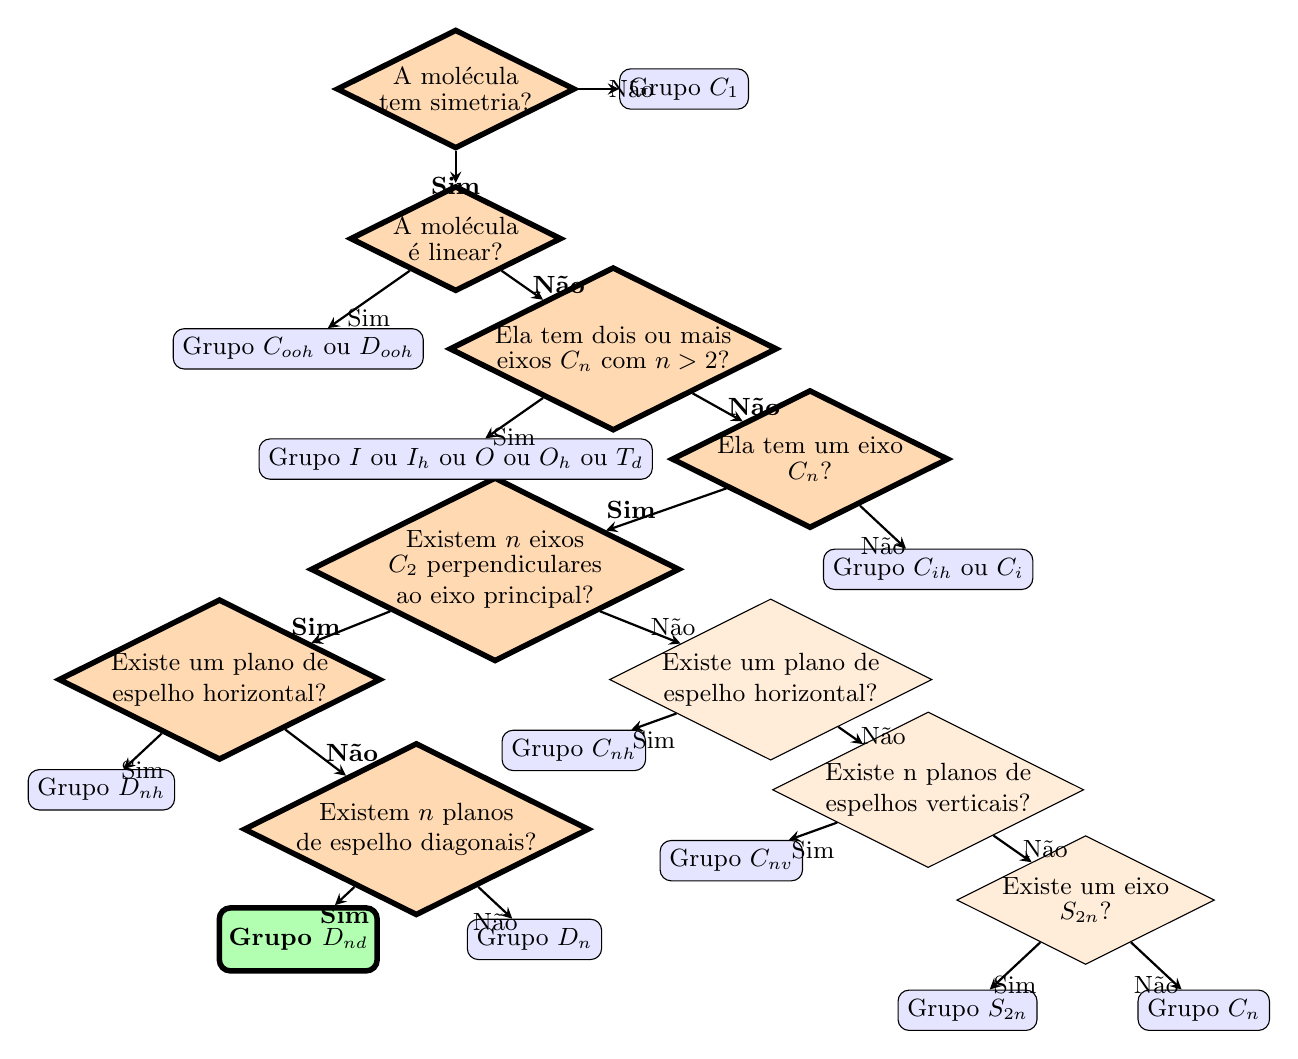
\begin{tikzpicture}[node distance=1.4cm]
			% Definindo as 15 decisões
			\node (Q_1) [decision_S, xshift=-7cm, line width=0.7mm] {\shortstack{A molécula\\tem simetria?}};
			\node (Q_2) [decision_S, below of=Q_1, yshift=-0.5cm, line width=0.7mm] {\shortstack{A molécula\\é linear?}};
			\node (Q_4) [decision_S, below of=Q_2, xshift=2cm, line width=0.7mm] {\shortstack{Ela tem dois ou mais\\eixos \( C_n \) com \( n>2 \)?}};
			\node (Q_6) [decision_S, below of=Q_4, xshift=2.5cm, line width=0.7mm] {\shortstack{Ela tem um eixo\\\( C_n \)?}};
			\node (Q_9) [decision_S, below of=Q_6, xshift=-4cm, line width=0.7mm] {\shortstack{Existem \( n \) eixos\\\( C_2 \) perpendiculares\\ao eixo principal?}};
			\node (Q_10) [decision_S, below of=Q_9, xshift=-3.5cm, line width=0.7mm] {\shortstack{Existe um plano de\\espelho horizontal?}};
			\node (Q_11) [decision_S, below of=Q_10, xshift=2.5cm, yshift=-0.5cm, line width=0.7mm] {\shortstack{Existem \( n \) planos\\de espelho diagonais?}};
			\node (Q_12) [decision, below of=Q_9, xshift=3.5cm] {\shortstack{Existe um plano de\\espelho horizontal?}};
			\node (Q_13) [decision, below of=Q_12, xshift=2cm] {\shortstack{Existe n planos de\\espelhos verticais?}};
			\node (Q_14) [decision, below of=Q_13, xshift=2cm] {\shortstack{Existe um eixo\\\( S_{2n} \)?}};

			% Caminhos
			\node (CooDoo) [startstop, below of=Q_2, xshift=-2cm] {Grupo $C_{ooh}$ ou $D_{ooh}$};
			\node (G_alta_simetria) [startstop, below of=Q_4, xshift=-2cm] {Grupo $I$ ou $I_h$ ou $O$ ou $O_h$ ou $T_d$};
			\node (G_baixa_simetria) [startstop, below of=Q_6, xshift=1.5cm] {Grupo $C_{ih}$ ou $C_i$};
			\node (Dnh) [startstop, below of=Q_10, xshift=-1.5cm] {Grupo $D_{nh}$};
			\node (Dnd) [startstop_S, below of=Q_11, xshift=-1.5cm, line width=0.7mm] {\textbf{Grupo $D_{nd}$}};
			\node (Dn) [startstop, below of=Q_11, xshift=1.5cm] {Grupo $D_n$};
			\node (Cnv) [startstop, below of=Q_13, xshift=-2.5cm, yshift=0.5cm] {Grupo $C_{nv}$};
			\node (Cnh) [startstop, below of=Q_12, xshift=-2.5cm, yshift=0.5cm] {Grupo $C_{nh}$};
			\node (S2n) [startstop, below of=Q_14, xshift=-1.5cm] {Grupo $S_{2n}$};
			\node (Cn) [startstop, below of=Q_14, xshift=1.5cm] {Grupo $C_n$};
			\node (C1) [startstop, right of=Q_1, xshift=1.5cm] {Grupo $C_1$};

			% Connections
			\draw [arrow] (Q_1) -- node[anchor=north, font=\small] {\textbf{Sim}} (Q_2);
			\draw [arrow] (Q_2) -- node[anchor=west, font=\small] {\textbf{Não}} (Q_4);
			\draw [arrow] (Q_4) -- node[anchor=west, font=\small] {\textbf{Não}} (Q_6);
			\draw [arrow] (Q_6) -- node[anchor=east, font=\small] {\textbf{Sim}} (Q_9);
			\draw [arrow] (Q_9) -- node[anchor=east, font=\small] {\textbf{Sim}} (Q_10);
			\draw [arrow] (Q_10) -- node[anchor=west, font=\small] {\textbf{Não}} (Q_11);
			\draw [arrow] (Q_9) -- node[anchor=west, font=\small] {Não} (Q_12);
			\draw [arrow] (Q_12) -- node[anchor=west, font=\small] {Não} (Q_13);
			\draw [arrow] (Q_13) -- node[anchor=west, font=\small] {Não} (Q_14);

			% Final Connections
			\draw [arrow] (Q_2) -- node[anchor=north, font=\small] {Sim} (CooDoo);
			\draw [arrow] (Q_4) -- node[anchor=north, font=\small] {Sim} (G_alta_simetria);
			\draw [arrow] (Q_6) -- node[anchor=north, font=\small] {Não} (G_baixa_simetria);
			\draw [arrow] (Q_10) -- node[anchor=north, font=\small] {Sim} (Dnh);
			\draw [arrow] (Q_11) -- node[anchor=north, font=\small] {\textbf{Sim}} (Dnd);
			\draw [arrow] (Q_11) -- node[anchor=north, font=\small] {Não} (Dn);
			\draw [arrow] (Q_12) -- node[anchor=north, font=\small] {Sim} (Cnh);
			\draw [arrow] (Q_13) -- node[anchor=north, font=\small] {Sim} (Cnv);
			\draw [arrow] (Q_14) -- node[anchor=north, font=\small] {Sim} (S2n);
			\draw [arrow] (Q_14) -- node[anchor=north, font=\small] {Não} (Cn);
			\draw [arrow] (Q_1) -- node[anchor=west, font=\small] {Não} (C1);

		\end{tikzpicture}
	\end{center}
\end{answer}

\begin{answer}[Ítem 2.2 - Tabela de Multiplicação]

Operações de Multiplicação:

\begin{longtable}{>{$}r<{$} >{$}l<{$} >{$}l<{$}}
                \makebox[3.3cm][r]{$\mathrm{\mathrm{E}} \circ \mathrm{\mathrm{E}}$} &= $\mathrm{\mathrm{E}} \circ [1, 2, 3, 4, 5, 6, 7, 8]$ &= $[1, 2, 3, 4, 5, 6, 7, 8]$ &= \makebox[2.3cm][l]{$\mathrm{\mathrm{E}}$} \\
\makebox[3.3cm][r]{$\mathrm{\mathrm{E}} \circ \mathrm{\mathrm{C}_{3}}$} &= $\mathrm{\mathrm{E}} \circ [1, 2, 4, 5, 3, 7, 8, 6]$ &= $[1, 2, 4, 5, 3, 7, 8, 6]$ &= \makebox[2.3cm][l]{$\mathrm{\mathrm{C}_{3}}$} \\
\makebox[3.3cm][r]{$\mathrm{\mathrm{E}} \circ \mathrm{\mathrm{C}_{3}^{2}}$} &= $\mathrm{\mathrm{E}} \circ [1, 2, 5, 3, 4, 8, 6, 7]$ &= $[1, 2, 5, 3, 4, 8, 6, 7]$ &= \makebox[2.3cm][l]{$\mathrm{\mathrm{C}_{3}^{2}}$} \\
\makebox[3.3cm][r]{$\mathrm{\mathrm{E}} \circ \mathrm{\mathrm{C}_{2}^{(a)}}$} &= $\mathrm{\mathrm{E}} \circ [2, 1, 8, 7, 6, 5, 4, 3]$ &= $[2, 1, 8, 7, 6, 5, 4, 3]$ &= \makebox[2.3cm][l]{$\mathrm{\mathrm{C}_{2}^{(a)}}$} \\
\makebox[3.3cm][r]{$\mathrm{\mathrm{E}} \circ \mathrm{\mathrm{C}_{2}^{(b)}}$} &= $\mathrm{\mathrm{E}} \circ [2, 1, 6, 8, 7, 3, 5, 4]$ &= $[2, 1, 6, 8, 7, 3, 5, 4]$ &= \makebox[2.3cm][l]{$\mathrm{\mathrm{C}_{2}^{(b)}}$} \\
\makebox[3.3cm][r]{$\mathrm{\mathrm{E}} \circ \mathrm{\mathrm{C}_{2}^{(c)}}$} &= $\mathrm{\mathrm{E}} \circ [2, 1, 7, 6, 8, 4, 3, 5]$ &= $[2, 1, 7, 6, 8, 4, 3, 5]$ &= \makebox[2.3cm][l]{$\mathrm{\mathrm{C}_{2}^{(c)}}$} \\
\makebox[3.3cm][r]{$\mathrm{\mathrm{E}} \circ \mathrm{\sigma_{d1}}$} &= $\mathrm{\mathrm{E}} \circ [1, 2, 3, 5, 4, 8, 7, 6]$ &= $[1, 2, 3, 5, 4, 8, 7, 6]$ &= \makebox[2.3cm][l]{$\mathrm{\sigma_{d1}}$} \\
\makebox[3.3cm][r]{$\mathrm{\mathrm{E}} \circ \mathrm{\sigma_{d2}}$} &= $\mathrm{\mathrm{E}} \circ [1, 2, 5, 4, 3, 7, 6, 8]$ &= $[1, 2, 5, 4, 3, 7, 6, 8]$ &= \makebox[2.3cm][l]{$\mathrm{\sigma_{d2}}$} \\
\makebox[3.3cm][r]{$\mathrm{\mathrm{E}} \circ \mathrm{\sigma_{d3}}$} &= $\mathrm{\mathrm{E}} \circ [1, 2, 4, 3, 5, 6, 8, 7]$ &= $[1, 2, 4, 3, 5, 6, 8, 7]$ &= \makebox[2.3cm][l]{$\mathrm{\sigma_{d3}}$} \\
\makebox[3.3cm][r]{$\mathrm{\mathrm{E}} \circ \mathrm{\mathrm{S}_{6}}$} &= $\mathrm{\mathrm{E}} \circ [2, 1, 6, 7, 8, 4, 5, 3]$ &= $[2, 1, 6, 7, 8, 4, 5, 3]$ &= \makebox[2.3cm][l]{$\mathrm{\mathrm{S}_{6}}$} \\
\makebox[3.3cm][r]{$\mathrm{\mathrm{E}} \circ \mathrm{\mathrm{S}_{6}^{5}}$} &= $\mathrm{\mathrm{E}} \circ [2, 1, 8, 6, 7, 3, 4, 5]$ &= $[2, 1, 8, 6, 7, 3, 4, 5]$ &= \makebox[2.3cm][l]{$\mathrm{\mathrm{S}_{6}^{5}}$} \\
\makebox[3.3cm][r]{$\mathrm{\mathrm{E}} \circ \mathrm{\mathrm{i}}$} &= $\mathrm{\mathrm{E}} \circ [2, 1, 7, 8, 6, 5, 3, 4]$ &= $[2, 1, 7, 8, 6, 5, 3, 4]$ &= \makebox[2.3cm][l]{$\mathrm{\mathrm{i}}$} \\
\makebox[3.3cm][r]{$\mathrm{\mathrm{C}_{3}} \circ \mathrm{\mathrm{E}}$} &= $\mathrm{\mathrm{C}_{3}} \circ [1, 2, 3, 4, 5, 6, 7, 8]$ &= $[1, 2, 4, 5, 3, 7, 8, 6]$ &= \makebox[2.3cm][l]{$\mathrm{\mathrm{C}_{3}}$} \\
\makebox[3.3cm][r]{$\mathrm{\mathrm{C}_{3}} \circ \mathrm{\mathrm{C}_{3}}$} &= $\mathrm{\mathrm{C}_{3}} \circ [1, 2, 4, 5, 3, 7, 8, 6]$ &= $[1, 2, 5, 3, 4, 8, 6, 7]$ &= \makebox[2.3cm][l]{$\mathrm{\mathrm{C}_{3}^{2}}$} \\
\makebox[3.3cm][r]{$\mathrm{\mathrm{C}_{3}} \circ \mathrm{\mathrm{C}_{3}^{2}}$} &= $\mathrm{\mathrm{C}_{3}} \circ [1, 2, 5, 3, 4, 8, 6, 7]$ &= $[1, 2, 3, 4, 5, 6, 7, 8]$ &= \makebox[2.3cm][l]{$\mathrm{\mathrm{E}}$} \\
\makebox[3.3cm][r]{$\mathrm{\mathrm{C}_{3}} \circ \mathrm{\mathrm{C}_{2}^{(a)}}$} &= $\mathrm{\mathrm{C}_{3}} \circ [2, 1, 8, 7, 6, 5, 4, 3]$ &= $[2, 1, 7, 6, 8, 4, 3, 5]$ &= \makebox[2.3cm][l]{$\mathrm{\mathrm{C}_{2}^{(c)}}$} \\
\makebox[3.3cm][r]{$\mathrm{\mathrm{C}_{3}} \circ \mathrm{\mathrm{C}_{2}^{(b)}}$} &= $\mathrm{\mathrm{C}_{3}} \circ [2, 1, 6, 8, 7, 3, 5, 4]$ &= $[2, 1, 8, 7, 6, 5, 4, 3]$ &= \makebox[2.3cm][l]{$\mathrm{\mathrm{C}_{2}^{(a)}}$} \\
\makebox[3.3cm][r]{$\mathrm{\mathrm{C}_{3}} \circ \mathrm{\mathrm{C}_{2}^{(c)}}$} &= $\mathrm{\mathrm{C}_{3}} \circ [2, 1, 7, 6, 8, 4, 3, 5]$ &= $[2, 1, 6, 8, 7, 3, 5, 4]$ &= \makebox[2.3cm][l]{$\mathrm{\mathrm{C}_{2}^{(b)}}$} \\
\makebox[3.3cm][r]{$\mathrm{\mathrm{C}_{3}} \circ \mathrm{\sigma_{d1}}$} &= $\mathrm{\mathrm{C}_{3}} \circ [1, 2, 3, 5, 4, 8, 7, 6]$ &= $[1, 2, 5, 4, 3, 7, 6, 8]$ &= \makebox[2.3cm][l]{$\mathrm{\sigma_{d2}}$} \\
\makebox[3.3cm][r]{$\mathrm{\mathrm{C}_{3}} \circ \mathrm{\sigma_{d2}}$} &= $\mathrm{\mathrm{C}_{3}} \circ [1, 2, 5, 4, 3, 7, 6, 8]$ &= $[1, 2, 4, 3, 5, 6, 8, 7]$ &= \makebox[2.3cm][l]{$\mathrm{\sigma_{d3}}$} \\
\makebox[3.3cm][r]{$\mathrm{\mathrm{C}_{3}} \circ \mathrm{\sigma_{d3}}$} &= $\mathrm{\mathrm{C}_{3}} \circ [1, 2, 4, 3, 5, 6, 8, 7]$ &= $[1, 2, 3, 5, 4, 8, 7, 6]$ &= \makebox[2.3cm][l]{$\mathrm{\sigma_{d1}}$} \\
\makebox[3.3cm][r]{$\mathrm{\mathrm{C}_{3}} \circ \mathrm{\mathrm{S}_{6}}$} &= $\mathrm{\mathrm{C}_{3}} \circ [2, 1, 6, 7, 8, 4, 5, 3]$ &= $[2, 1, 7, 8, 6, 5, 3, 4]$ &= \makebox[2.3cm][l]{$\mathrm{\mathrm{i}}$} \\
\makebox[3.3cm][r]{$\mathrm{\mathrm{C}_{3}} \circ \mathrm{\mathrm{S}_{6}^{5}}$} &= $\mathrm{\mathrm{C}_{3}} \circ [2, 1, 8, 6, 7, 3, 4, 5]$ &= $[2, 1, 6, 7, 8, 4, 5, 3]$ &= \makebox[2.3cm][l]{$\mathrm{\mathrm{S}_{6}}$} \\
\makebox[3.3cm][r]{$\mathrm{\mathrm{C}_{3}} \circ \mathrm{\mathrm{i}}$} &= $\mathrm{\mathrm{C}_{3}} \circ [2, 1, 7, 8, 6, 5, 3, 4]$ &= $[2, 1, 8, 6, 7, 3, 4, 5]$ &= \makebox[2.3cm][l]{$\mathrm{\mathrm{S}_{6}^{5}}$} \\
\makebox[3.3cm][r]{$\mathrm{\mathrm{C}_{3}^{2}} \circ \mathrm{\mathrm{E}}$} &= $\mathrm{\mathrm{C}_{3}^{2}} \circ [1, 2, 3, 4, 5, 6, 7, 8]$ &= $[1, 2, 5, 3, 4, 8, 6, 7]$ &= \makebox[2.3cm][l]{$\mathrm{\mathrm{C}_{3}^{2}}$} \\
\makebox[3.3cm][r]{$\mathrm{\mathrm{C}_{3}^{2}} \circ \mathrm{\mathrm{C}_{3}}$} &= $\mathrm{\mathrm{C}_{3}^{2}} \circ [1, 2, 4, 5, 3, 7, 8, 6]$ &= $[1, 2, 3, 4, 5, 6, 7, 8]$ &= \makebox[2.3cm][l]{$\mathrm{\mathrm{E}}$} \\
\makebox[3.3cm][r]{$\mathrm{\mathrm{C}_{3}^{2}} \circ \mathrm{\mathrm{C}_{3}^{2}}$} &= $\mathrm{\mathrm{C}_{3}^{2}} \circ [1, 2, 5, 3, 4, 8, 6, 7]$ &= $[1, 2, 4, 5, 3, 7, 8, 6]$ &= \makebox[2.3cm][l]{$\mathrm{\mathrm{C}_{3}}$} \\
\makebox[3.3cm][r]{$\mathrm{\mathrm{C}_{3}^{2}} \circ \mathrm{\mathrm{C}_{2}^{(a)}}$} &= $\mathrm{\mathrm{C}_{3}^{2}} \circ [2, 1, 8, 7, 6, 5, 4, 3]$ &= $[2, 1, 6, 8, 7, 3, 5, 4]$ &= \makebox[2.3cm][l]{$\mathrm{\mathrm{C}_{2}^{(b)}}$} \\
\makebox[3.3cm][r]{$\mathrm{\mathrm{C}_{3}^{2}} \circ \mathrm{\mathrm{C}_{2}^{(b)}}$} &= $\mathrm{\mathrm{C}_{3}^{2}} \circ [2, 1, 6, 8, 7, 3, 5, 4]$ &= $[2, 1, 7, 6, 8, 4, 3, 5]$ &= \makebox[2.3cm][l]{$\mathrm{\mathrm{C}_{2}^{(c)}}$} \\
\makebox[3.3cm][r]{$\mathrm{\mathrm{C}_{3}^{2}} \circ \mathrm{\mathrm{C}_{2}^{(c)}}$} &= $\mathrm{\mathrm{C}_{3}^{2}} \circ [2, 1, 7, 6, 8, 4, 3, 5]$ &= $[2, 1, 8, 7, 6, 5, 4, 3]$ &= \makebox[2.3cm][l]{$\mathrm{\mathrm{C}_{2}^{(a)}}$} \\
\makebox[3.3cm][r]{$\mathrm{\mathrm{C}_{3}^{2}} \circ \mathrm{\sigma_{d1}}$} &= $\mathrm{\mathrm{C}_{3}^{2}} \circ [1, 2, 3, 5, 4, 8, 7, 6]$ &= $[1, 2, 4, 3, 5, 6, 8, 7]$ &= \makebox[2.3cm][l]{$\mathrm{\sigma_{d3}}$} \\
\makebox[3.3cm][r]{$\mathrm{\mathrm{C}_{3}^{2}} \circ \mathrm{\sigma_{d2}}$} &= $\mathrm{\mathrm{C}_{3}^{2}} \circ [1, 2, 5, 4, 3, 7, 6, 8]$ &= $[1, 2, 3, 5, 4, 8, 7, 6]$ &= \makebox[2.3cm][l]{$\mathrm{\sigma_{d1}}$} \\
\makebox[3.3cm][r]{$\mathrm{\mathrm{C}_{3}^{2}} \circ \mathrm{\sigma_{d3}}$} &= $\mathrm{\mathrm{C}_{3}^{2}} \circ [1, 2, 4, 3, 5, 6, 8, 7]$ &= $[1, 2, 5, 4, 3, 7, 6, 8]$ &= \makebox[2.3cm][l]{$\mathrm{\sigma_{d2}}$} \\
\makebox[3.3cm][r]{$\mathrm{\mathrm{C}_{3}^{2}} \circ \mathrm{\mathrm{S}_{6}}$} &= $\mathrm{\mathrm{C}_{3}^{2}} \circ [2, 1, 6, 7, 8, 4, 5, 3]$ &= $[2, 1, 8, 6, 7, 3, 4, 5]$ &= \makebox[2.3cm][l]{$\mathrm{\mathrm{S}_{6}^{5}}$} \\
\makebox[3.3cm][r]{$\mathrm{\mathrm{C}_{3}^{2}} \circ \mathrm{\mathrm{S}_{6}^{5}}$} &= $\mathrm{\mathrm{C}_{3}^{2}} \circ [2, 1, 8, 6, 7, 3, 4, 5]$ &= $[2, 1, 7, 8, 6, 5, 3, 4]$ &= \makebox[2.3cm][l]{$\mathrm{\mathrm{i}}$} \\
\makebox[3.3cm][r]{$\mathrm{\mathrm{C}_{3}^{2}} \circ \mathrm{\mathrm{i}}$} &= $\mathrm{\mathrm{C}_{3}^{2}} \circ [2, 1, 7, 8, 6, 5, 3, 4]$ &= $[2, 1, 6, 7, 8, 4, 5, 3]$ &= \makebox[2.3cm][l]{$\mathrm{\mathrm{S}_{6}}$} \\
\makebox[3.3cm][r]{$\mathrm{\mathrm{C}_{2}^{(a)}} \circ \mathrm{\mathrm{E}}$} &= $\mathrm{\mathrm{C}_{2}^{(a)}} \circ [1, 2, 3, 4, 5, 6, 7, 8]$ &= $[2, 1, 8, 7, 6, 5, 4, 3]$ &= \makebox[2.3cm][l]{$\mathrm{\mathrm{C}_{2}^{(a)}}$} \\
\makebox[3.3cm][r]{$\mathrm{\mathrm{C}_{2}^{(a)}} \circ \mathrm{\mathrm{C}_{3}}$} &= $\mathrm{\mathrm{C}_{2}^{(a)}} \circ [1, 2, 4, 5, 3, 7, 8, 6]$ &= $[2, 1, 6, 8, 7, 3, 5, 4]$ &= \makebox[2.3cm][l]{$\mathrm{\mathrm{C}_{2}^{(b)}}$} \\
\makebox[3.3cm][r]{$\mathrm{\mathrm{C}_{2}^{(a)}} \circ \mathrm{\mathrm{C}_{3}^{2}}$} &= $\mathrm{\mathrm{C}_{2}^{(a)}} \circ [1, 2, 5, 3, 4, 8, 6, 7]$ &= $[2, 1, 7, 6, 8, 4, 3, 5]$ &= \makebox[2.3cm][l]{$\mathrm{\mathrm{C}_{2}^{(c)}}$} \\
\makebox[3.3cm][r]{$\mathrm{\mathrm{C}_{2}^{(a)}} \circ \mathrm{\mathrm{C}_{2}^{(a)}}$} &= $\mathrm{\mathrm{C}_{2}^{(a)}} \circ [2, 1, 8, 7, 6, 5, 4, 3]$ &= $[1, 2, 3, 4, 5, 6, 7, 8]$ &= \makebox[2.3cm][l]{$\mathrm{\mathrm{E}}$} \\
\makebox[3.3cm][r]{$\mathrm{\mathrm{C}_{2}^{(a)}} \circ \mathrm{\mathrm{C}_{2}^{(b)}}$} &= $\mathrm{\mathrm{C}_{2}^{(a)}} \circ [2, 1, 6, 8, 7, 3, 5, 4]$ &= $[1, 2, 4, 5, 3, 7, 8, 6]$ &= \makebox[2.3cm][l]{$\mathrm{\mathrm{C}_{3}}$} \\
\makebox[3.3cm][r]{$\mathrm{\mathrm{C}_{2}^{(a)}} \circ \mathrm{\mathrm{C}_{2}^{(c)}}$} &= $\mathrm{\mathrm{C}_{2}^{(a)}} \circ [2, 1, 7, 6, 8, 4, 3, 5]$ &= $[1, 2, 5, 3, 4, 8, 6, 7]$ &= \makebox[2.3cm][l]{$\mathrm{\mathrm{C}_{3}^{2}}$} \\
\makebox[3.3cm][r]{$\mathrm{\mathrm{C}_{2}^{(a)}} \circ \mathrm{\sigma_{d1}}$} &= $\mathrm{\mathrm{C}_{2}^{(a)}} \circ [1, 2, 3, 5, 4, 8, 7, 6]$ &= $[2, 1, 6, 7, 8, 4, 5, 3]$ &= \makebox[2.3cm][l]{$\mathrm{\mathrm{S}_{6}}$} \\
\makebox[3.3cm][r]{$\mathrm{\mathrm{C}_{2}^{(a)}} \circ \mathrm{\sigma_{d2}}$} &= $\mathrm{\mathrm{C}_{2}^{(a)}} \circ [1, 2, 5, 4, 3, 7, 6, 8]$ &= $[2, 1, 8, 6, 7, 3, 4, 5]$ &= \makebox[2.3cm][l]{$\mathrm{\mathrm{S}_{6}^{5}}$} \\
\makebox[3.3cm][r]{$\mathrm{\mathrm{C}_{2}^{(a)}} \circ \mathrm{\sigma_{d3}}$} &= $\mathrm{\mathrm{C}_{2}^{(a)}} \circ [1, 2, 4, 3, 5, 6, 8, 7]$ &= $[2, 1, 7, 8, 6, 5, 3, 4]$ &= \makebox[2.3cm][l]{$\mathrm{\mathrm{i}}$} \\
\makebox[3.3cm][r]{$\mathrm{\mathrm{C}_{2}^{(a)}} \circ \mathrm{\mathrm{S}_{6}}$} &= $\mathrm{\mathrm{C}_{2}^{(a)}} \circ [2, 1, 6, 7, 8, 4, 5, 3]$ &= $[1, 2, 3, 5, 4, 8, 7, 6]$ &= \makebox[2.3cm][l]{$\mathrm{\sigma_{d1}}$} \\
\makebox[3.3cm][r]{$\mathrm{\mathrm{C}_{2}^{(a)}} \circ \mathrm{\mathrm{S}_{6}^{5}}$} &= $\mathrm{\mathrm{C}_{2}^{(a)}} \circ [2, 1, 8, 6, 7, 3, 4, 5]$ &= $[1, 2, 5, 4, 3, 7, 6, 8]$ &= \makebox[2.3cm][l]{$\mathrm{\sigma_{d2}}$} \\
\makebox[3.3cm][r]{$\mathrm{\mathrm{C}_{2}^{(a)}} \circ \mathrm{\mathrm{i}}$} &= $\mathrm{\mathrm{C}_{2}^{(a)}} \circ [2, 1, 7, 8, 6, 5, 3, 4]$ &= $[1, 2, 4, 3, 5, 6, 8, 7]$ &= \makebox[2.3cm][l]{$\mathrm{\sigma_{d3}}$} \\
\makebox[3.3cm][r]{$\mathrm{\mathrm{C}_{2}^{(b)}} \circ \mathrm{\mathrm{E}}$} &= $\mathrm{\mathrm{C}_{2}^{(b)}} \circ [1, 2, 3, 4, 5, 6, 7, 8]$ &= $[2, 1, 6, 8, 7, 3, 5, 4]$ &= \makebox[2.3cm][l]{$\mathrm{\mathrm{C}_{2}^{(b)}}$} \\
\makebox[3.3cm][r]{$\mathrm{\mathrm{C}_{2}^{(b)}} \circ \mathrm{\mathrm{C}_{3}}$} &= $\mathrm{\mathrm{C}_{2}^{(b)}} \circ [1, 2, 4, 5, 3, 7, 8, 6]$ &= $[2, 1, 7, 6, 8, 4, 3, 5]$ &= \makebox[2.3cm][l]{$\mathrm{\mathrm{C}_{2}^{(c)}}$} \\
\makebox[3.3cm][r]{$\mathrm{\mathrm{C}_{2}^{(b)}} \circ \mathrm{\mathrm{C}_{3}^{2}}$} &= $\mathrm{\mathrm{C}_{2}^{(b)}} \circ [1, 2, 5, 3, 4, 8, 6, 7]$ &= $[2, 1, 8, 7, 6, 5, 4, 3]$ &= \makebox[2.3cm][l]{$\mathrm{\mathrm{C}_{2}^{(a)}}$} \\
\makebox[3.3cm][r]{$\mathrm{\mathrm{C}_{2}^{(b)}} \circ \mathrm{\mathrm{C}_{2}^{(a)}}$} &= $\mathrm{\mathrm{C}_{2}^{(b)}} \circ [2, 1, 8, 7, 6, 5, 4, 3]$ &= $[1, 2, 5, 3, 4, 8, 6, 7]$ &= \makebox[2.3cm][l]{$\mathrm{\mathrm{C}_{3}^{2}}$} \\
\makebox[3.3cm][r]{$\mathrm{\mathrm{C}_{2}^{(b)}} \circ \mathrm{\mathrm{C}_{2}^{(b)}}$} &= $\mathrm{\mathrm{C}_{2}^{(b)}} \circ [2, 1, 6, 8, 7, 3, 5, 4]$ &= $[1, 2, 3, 4, 5, 6, 7, 8]$ &= \makebox[2.3cm][l]{$\mathrm{\mathrm{E}}$} \\
\makebox[3.3cm][r]{$\mathrm{\mathrm{C}_{2}^{(b)}} \circ \mathrm{\mathrm{C}_{2}^{(c)}}$} &= $\mathrm{\mathrm{C}_{2}^{(b)}} \circ [2, 1, 7, 6, 8, 4, 3, 5]$ &= $[1, 2, 4, 5, 3, 7, 8, 6]$ &= \makebox[2.3cm][l]{$\mathrm{\mathrm{C}_{3}}$} \\
\makebox[3.3cm][r]{$\mathrm{\mathrm{C}_{2}^{(b)}} \circ \mathrm{\sigma_{d1}}$} &= $\mathrm{\mathrm{C}_{2}^{(b)}} \circ [1, 2, 3, 5, 4, 8, 7, 6]$ &= $[2, 1, 8, 6, 7, 3, 4, 5]$ &= \makebox[2.3cm][l]{$\mathrm{\mathrm{S}_{6}^{5}}$} \\
\makebox[3.3cm][r]{$\mathrm{\mathrm{C}_{2}^{(b)}} \circ \mathrm{\sigma_{d2}}$} &= $\mathrm{\mathrm{C}_{2}^{(b)}} \circ [1, 2, 5, 4, 3, 7, 6, 8]$ &= $[2, 1, 7, 8, 6, 5, 3, 4]$ &= \makebox[2.3cm][l]{$\mathrm{\mathrm{i}}$} \\
\makebox[3.3cm][r]{$\mathrm{\mathrm{C}_{2}^{(b)}} \circ \mathrm{\sigma_{d3}}$} &= $\mathrm{\mathrm{C}_{2}^{(b)}} \circ [1, 2, 4, 3, 5, 6, 8, 7]$ &= $[2, 1, 6, 7, 8, 4, 5, 3]$ &= \makebox[2.3cm][l]{$\mathrm{\mathrm{S}_{6}}$} \\
\makebox[3.3cm][r]{$\mathrm{\mathrm{C}_{2}^{(b)}} \circ \mathrm{\mathrm{S}_{6}}$} &= $\mathrm{\mathrm{C}_{2}^{(b)}} \circ [2, 1, 6, 7, 8, 4, 5, 3]$ &= $[1, 2, 4, 3, 5, 6, 8, 7]$ &= \makebox[2.3cm][l]{$\mathrm{\sigma_{d3}}$} \\
\makebox[3.3cm][r]{$\mathrm{\mathrm{C}_{2}^{(b)}} \circ \mathrm{\mathrm{S}_{6}^{5}}$} &= $\mathrm{\mathrm{C}_{2}^{(b)}} \circ [2, 1, 8, 6, 7, 3, 4, 5]$ &= $[1, 2, 3, 5, 4, 8, 7, 6]$ &= \makebox[2.3cm][l]{$\mathrm{\sigma_{d1}}$} \\
\makebox[3.3cm][r]{$\mathrm{\mathrm{C}_{2}^{(b)}} \circ \mathrm{\mathrm{i}}$} &= $\mathrm{\mathrm{C}_{2}^{(b)}} \circ [2, 1, 7, 8, 6, 5, 3, 4]$ &= $[1, 2, 5, 4, 3, 7, 6, 8]$ &= \makebox[2.3cm][l]{$\mathrm{\sigma_{d2}}$} \\
\makebox[3.3cm][r]{$\mathrm{\mathrm{C}_{2}^{(c)}} \circ \mathrm{\mathrm{E}}$} &= $\mathrm{\mathrm{C}_{2}^{(c)}} \circ [1, 2, 3, 4, 5, 6, 7, 8]$ &= $[2, 1, 7, 6, 8, 4, 3, 5]$ &= \makebox[2.3cm][l]{$\mathrm{\mathrm{C}_{2}^{(c)}}$} \\
\makebox[3.3cm][r]{$\mathrm{\mathrm{C}_{2}^{(c)}} \circ \mathrm{\mathrm{C}_{3}}$} &= $\mathrm{\mathrm{C}_{2}^{(c)}} \circ [1, 2, 4, 5, 3, 7, 8, 6]$ &= $[2, 1, 8, 7, 6, 5, 4, 3]$ &= \makebox[2.3cm][l]{$\mathrm{\mathrm{C}_{2}^{(a)}}$} \\
\makebox[3.3cm][r]{$\mathrm{\mathrm{C}_{2}^{(c)}} \circ \mathrm{\mathrm{C}_{3}^{2}}$} &= $\mathrm{\mathrm{C}_{2}^{(c)}} \circ [1, 2, 5, 3, 4, 8, 6, 7]$ &= $[2, 1, 6, 8, 7, 3, 5, 4]$ &= \makebox[2.3cm][l]{$\mathrm{\mathrm{C}_{2}^{(b)}}$} \\
\makebox[3.3cm][r]{$\mathrm{\mathrm{C}_{2}^{(c)}} \circ \mathrm{\mathrm{C}_{2}^{(a)}}$} &= $\mathrm{\mathrm{C}_{2}^{(c)}} \circ [2, 1, 8, 7, 6, 5, 4, 3]$ &= $[1, 2, 4, 5, 3, 7, 8, 6]$ &= \makebox[2.3cm][l]{$\mathrm{\mathrm{C}_{3}}$} \\
\makebox[3.3cm][r]{$\mathrm{\mathrm{C}_{2}^{(c)}} \circ \mathrm{\mathrm{C}_{2}^{(b)}}$} &= $\mathrm{\mathrm{C}_{2}^{(c)}} \circ [2, 1, 6, 8, 7, 3, 5, 4]$ &= $[1, 2, 5, 3, 4, 8, 6, 7]$ &= \makebox[2.3cm][l]{$\mathrm{\mathrm{C}_{3}^{2}}$} \\
\makebox[3.3cm][r]{$\mathrm{\mathrm{C}_{2}^{(c)}} \circ \mathrm{\mathrm{C}_{2}^{(c)}}$} &= $\mathrm{\mathrm{C}_{2}^{(c)}} \circ [2, 1, 7, 6, 8, 4, 3, 5]$ &= $[1, 2, 3, 4, 5, 6, 7, 8]$ &= \makebox[2.3cm][l]{$\mathrm{\mathrm{E}}$} \\
\makebox[3.3cm][r]{$\mathrm{\mathrm{C}_{2}^{(c)}} \circ \mathrm{\sigma_{d1}}$} &= $\mathrm{\mathrm{C}_{2}^{(c)}} \circ [1, 2, 3, 5, 4, 8, 7, 6]$ &= $[2, 1, 7, 8, 6, 5, 3, 4]$ &= \makebox[2.3cm][l]{$\mathrm{\mathrm{i}}$} \\
\makebox[3.3cm][r]{$\mathrm{\mathrm{C}_{2}^{(c)}} \circ \mathrm{\sigma_{d2}}$} &= $\mathrm{\mathrm{C}_{2}^{(c)}} \circ [1, 2, 5, 4, 3, 7, 6, 8]$ &= $[2, 1, 6, 7, 8, 4, 5, 3]$ &= \makebox[2.3cm][l]{$\mathrm{\mathrm{S}_{6}}$} \\
\makebox[3.3cm][r]{$\mathrm{\mathrm{C}_{2}^{(c)}} \circ \mathrm{\sigma_{d3}}$} &= $\mathrm{\mathrm{C}_{2}^{(c)}} \circ [1, 2, 4, 3, 5, 6, 8, 7]$ &= $[2, 1, 8, 6, 7, 3, 4, 5]$ &= \makebox[2.3cm][l]{$\mathrm{\mathrm{S}_{6}^{5}}$} \\
\makebox[3.3cm][r]{$\mathrm{\mathrm{C}_{2}^{(c)}} \circ \mathrm{\mathrm{S}_{6}}$} &= $\mathrm{\mathrm{C}_{2}^{(c)}} \circ [2, 1, 6, 7, 8, 4, 5, 3]$ &= $[1, 2, 5, 4, 3, 7, 6, 8]$ &= \makebox[2.3cm][l]{$\mathrm{\sigma_{d2}}$} \\
\makebox[3.3cm][r]{$\mathrm{\mathrm{C}_{2}^{(c)}} \circ \mathrm{\mathrm{S}_{6}^{5}}$} &= $\mathrm{\mathrm{C}_{2}^{(c)}} \circ [2, 1, 8, 6, 7, 3, 4, 5]$ &= $[1, 2, 4, 3, 5, 6, 8, 7]$ &= \makebox[2.3cm][l]{$\mathrm{\sigma_{d3}}$} \\
\makebox[3.3cm][r]{$\mathrm{\mathrm{C}_{2}^{(c)}} \circ \mathrm{\mathrm{i}}$} &= $\mathrm{\mathrm{C}_{2}^{(c)}} \circ [2, 1, 7, 8, 6, 5, 3, 4]$ &= $[1, 2, 3, 5, 4, 8, 7, 6]$ &= \makebox[2.3cm][l]{$\mathrm{\sigma_{d1}}$} \\
\makebox[3.3cm][r]{$\mathrm{\sigma_{d1}} \circ \mathrm{\mathrm{E}}$} &= $\mathrm{\sigma_{d1}} \circ [1, 2, 3, 4, 5, 6, 7, 8]$ &= $[1, 2, 3, 5, 4, 8, 7, 6]$ &= \makebox[2.3cm][l]{$\mathrm{\sigma_{d1}}$} \\
\makebox[3.3cm][r]{$\mathrm{\sigma_{d1}} \circ \mathrm{\mathrm{C}_{3}}$} &= $\mathrm{\sigma_{d1}} \circ [1, 2, 4, 5, 3, 7, 8, 6]$ &= $[1, 2, 4, 3, 5, 6, 8, 7]$ &= \makebox[2.3cm][l]{$\mathrm{\sigma_{d3}}$} \\
\makebox[3.3cm][r]{$\mathrm{\sigma_{d1}} \circ \mathrm{\mathrm{C}_{3}^{2}}$} &= $\mathrm{\sigma_{d1}} \circ [1, 2, 5, 3, 4, 8, 6, 7]$ &= $[1, 2, 5, 4, 3, 7, 6, 8]$ &= \makebox[2.3cm][l]{$\mathrm{\sigma_{d2}}$} \\
\makebox[3.3cm][r]{$\mathrm{\sigma_{d1}} \circ \mathrm{\mathrm{C}_{2}^{(a)}}$} &= $\mathrm{\sigma_{d1}} \circ [2, 1, 8, 7, 6, 5, 4, 3]$ &= $[2, 1, 8, 6, 7, 3, 4, 5]$ &= \makebox[2.3cm][l]{$\mathrm{\mathrm{S}_{6}^{5}}$} \\
\makebox[3.3cm][r]{$\mathrm{\sigma_{d1}} \circ \mathrm{\mathrm{C}_{2}^{(b)}}$} &= $\mathrm{\sigma_{d1}} \circ [2, 1, 6, 8, 7, 3, 5, 4]$ &= $[2, 1, 6, 7, 8, 4, 5, 3]$ &= \makebox[2.3cm][l]{$\mathrm{\mathrm{S}_{6}}$} \\
\makebox[3.3cm][r]{$\mathrm{\sigma_{d1}} \circ \mathrm{\mathrm{C}_{2}^{(c)}}$} &= $\mathrm{\sigma_{d1}} \circ [2, 1, 7, 6, 8, 4, 3, 5]$ &= $[2, 1, 7, 8, 6, 5, 3, 4]$ &= \makebox[2.3cm][l]{$\mathrm{\mathrm{i}}$} \\
\makebox[3.3cm][r]{$\mathrm{\sigma_{d1}} \circ \mathrm{\sigma_{d1}}$} &= $\mathrm{\sigma_{d1}} \circ [1, 2, 3, 5, 4, 8, 7, 6]$ &= $[1, 2, 3, 4, 5, 6, 7, 8]$ &= \makebox[2.3cm][l]{$\mathrm{\mathrm{E}}$} \\
\makebox[3.3cm][r]{$\mathrm{\sigma_{d1}} \circ \mathrm{\sigma_{d2}}$} &= $\mathrm{\sigma_{d1}} \circ [1, 2, 5, 4, 3, 7, 6, 8]$ &= $[1, 2, 5, 3, 4, 8, 6, 7]$ &= \makebox[2.3cm][l]{$\mathrm{\mathrm{C}_{3}^{2}}$} \\
\makebox[3.3cm][r]{$\mathrm{\sigma_{d1}} \circ \mathrm{\sigma_{d3}}$} &= $\mathrm{\sigma_{d1}} \circ [1, 2, 4, 3, 5, 6, 8, 7]$ &= $[1, 2, 4, 5, 3, 7, 8, 6]$ &= \makebox[2.3cm][l]{$\mathrm{\mathrm{C}_{3}}$} \\
\makebox[3.3cm][r]{$\mathrm{\sigma_{d1}} \circ \mathrm{\mathrm{S}_{6}}$} &= $\mathrm{\sigma_{d1}} \circ [2, 1, 6, 7, 8, 4, 5, 3]$ &= $[2, 1, 6, 8, 7, 3, 5, 4]$ &= \makebox[2.3cm][l]{$\mathrm{\mathrm{C}_{2}^{(b)}}$} \\
\makebox[3.3cm][r]{$\mathrm{\sigma_{d1}} \circ \mathrm{\mathrm{S}_{6}^{5}}$} &= $\mathrm{\sigma_{d1}} \circ [2, 1, 8, 6, 7, 3, 4, 5]$ &= $[2, 1, 8, 7, 6, 5, 4, 3]$ &= \makebox[2.3cm][l]{$\mathrm{\mathrm{C}_{2}^{(a)}}$} \\
\makebox[3.3cm][r]{$\mathrm{\sigma_{d1}} \circ \mathrm{\mathrm{i}}$} &= $\mathrm{\sigma_{d1}} \circ [2, 1, 7, 8, 6, 5, 3, 4]$ &= $[2, 1, 7, 6, 8, 4, 3, 5]$ &= \makebox[2.3cm][l]{$\mathrm{\mathrm{C}_{2}^{(c)}}$} \\
\makebox[3.3cm][r]{$\mathrm{\sigma_{d2}} \circ \mathrm{\mathrm{E}}$} &= $\mathrm{\sigma_{d2}} \circ [1, 2, 3, 4, 5, 6, 7, 8]$ &= $[1, 2, 5, 4, 3, 7, 6, 8]$ &= \makebox[2.3cm][l]{$\mathrm{\sigma_{d2}}$} \\
\makebox[3.3cm][r]{$\mathrm{\sigma_{d2}} \circ \mathrm{\mathrm{C}_{3}}$} &= $\mathrm{\sigma_{d2}} \circ [1, 2, 4, 5, 3, 7, 8, 6]$ &= $[1, 2, 3, 5, 4, 8, 7, 6]$ &= \makebox[2.3cm][l]{$\mathrm{\sigma_{d1}}$} \\
\makebox[3.3cm][r]{$\mathrm{\sigma_{d2}} \circ \mathrm{\mathrm{C}_{3}^{2}}$} &= $\mathrm{\sigma_{d2}} \circ [1, 2, 5, 3, 4, 8, 6, 7]$ &= $[1, 2, 4, 3, 5, 6, 8, 7]$ &= \makebox[2.3cm][l]{$\mathrm{\sigma_{d3}}$} \\
\makebox[3.3cm][r]{$\mathrm{\sigma_{d2}} \circ \mathrm{\mathrm{C}_{2}^{(a)}}$} &= $\mathrm{\sigma_{d2}} \circ [2, 1, 8, 7, 6, 5, 4, 3]$ &= $[2, 1, 6, 7, 8, 4, 5, 3]$ &= \makebox[2.3cm][l]{$\mathrm{\mathrm{S}_{6}}$} \\
\makebox[3.3cm][r]{$\mathrm{\sigma_{d2}} \circ \mathrm{\mathrm{C}_{2}^{(b)}}$} &= $\mathrm{\sigma_{d2}} \circ [2, 1, 6, 8, 7, 3, 5, 4]$ &= $[2, 1, 7, 8, 6, 5, 3, 4]$ &= \makebox[2.3cm][l]{$\mathrm{\mathrm{i}}$} \\
\makebox[3.3cm][r]{$\mathrm{\sigma_{d2}} \circ \mathrm{\mathrm{C}_{2}^{(c)}}$} &= $\mathrm{\sigma_{d2}} \circ [2, 1, 7, 6, 8, 4, 3, 5]$ &= $[2, 1, 8, 6, 7, 3, 4, 5]$ &= \makebox[2.3cm][l]{$\mathrm{\mathrm{S}_{6}^{5}}$} \\
\makebox[3.3cm][r]{$\mathrm{\sigma_{d2}} \circ \mathrm{\sigma_{d1}}$} &= $\mathrm{\sigma_{d2}} \circ [1, 2, 3, 5, 4, 8, 7, 6]$ &= $[1, 2, 4, 5, 3, 7, 8, 6]$ &= \makebox[2.3cm][l]{$\mathrm{\mathrm{C}_{3}}$} \\
\makebox[3.3cm][r]{$\mathrm{\sigma_{d2}} \circ \mathrm{\sigma_{d2}}$} &= $\mathrm{\sigma_{d2}} \circ [1, 2, 5, 4, 3, 7, 6, 8]$ &= $[1, 2, 3, 4, 5, 6, 7, 8]$ &= \makebox[2.3cm][l]{$\mathrm{\mathrm{E}}$} \\
\makebox[3.3cm][r]{$\mathrm{\sigma_{d2}} \circ \mathrm{\sigma_{d3}}$} &= $\mathrm{\sigma_{d2}} \circ [1, 2, 4, 3, 5, 6, 8, 7]$ &= $[1, 2, 5, 3, 4, 8, 6, 7]$ &= \makebox[2.3cm][l]{$\mathrm{\mathrm{C}_{3}^{2}}$} \\
\makebox[3.3cm][r]{$\mathrm{\sigma_{d2}} \circ \mathrm{\mathrm{S}_{6}}$} &= $\mathrm{\sigma_{d2}} \circ [2, 1, 6, 7, 8, 4, 5, 3]$ &= $[2, 1, 8, 7, 6, 5, 4, 3]$ &= \makebox[2.3cm][l]{$\mathrm{\mathrm{C}_{2}^{(a)}}$} \\
\makebox[3.3cm][r]{$\mathrm{\sigma_{d2}} \circ \mathrm{\mathrm{S}_{6}^{5}}$} &= $\mathrm{\sigma_{d2}} \circ [2, 1, 8, 6, 7, 3, 4, 5]$ &= $[2, 1, 7, 6, 8, 4, 3, 5]$ &= \makebox[2.3cm][l]{$\mathrm{\mathrm{C}_{2}^{(c)}}$} \\
\makebox[3.3cm][r]{$\mathrm{\sigma_{d2}} \circ \mathrm{\mathrm{i}}$} &= $\mathrm{\sigma_{d2}} \circ [2, 1, 7, 8, 6, 5, 3, 4]$ &= $[2, 1, 6, 8, 7, 3, 5, 4]$ &= \makebox[2.3cm][l]{$\mathrm{\mathrm{C}_{2}^{(b)}}$} \\
\makebox[3.3cm][r]{$\mathrm{\sigma_{d3}} \circ \mathrm{\mathrm{E}}$} &= $\mathrm{\sigma_{d3}} \circ [1, 2, 3, 4, 5, 6, 7, 8]$ &= $[1, 2, 4, 3, 5, 6, 8, 7]$ &= \makebox[2.3cm][l]{$\mathrm{\sigma_{d3}}$} \\
\makebox[3.3cm][r]{$\mathrm{\sigma_{d3}} \circ \mathrm{\mathrm{C}_{3}}$} &= $\mathrm{\sigma_{d3}} \circ [1, 2, 4, 5, 3, 7, 8, 6]$ &= $[1, 2, 5, 4, 3, 7, 6, 8]$ &= \makebox[2.3cm][l]{$\mathrm{\sigma_{d2}}$} \\
\makebox[3.3cm][r]{$\mathrm{\sigma_{d3}} \circ \mathrm{\mathrm{C}_{3}^{2}}$} &= $\mathrm{\sigma_{d3}} \circ [1, 2, 5, 3, 4, 8, 6, 7]$ &= $[1, 2, 3, 5, 4, 8, 7, 6]$ &= \makebox[2.3cm][l]{$\mathrm{\sigma_{d1}}$} \\
\makebox[3.3cm][r]{$\mathrm{\sigma_{d3}} \circ \mathrm{\mathrm{C}_{2}^{(a)}}$} &= $\mathrm{\sigma_{d3}} \circ [2, 1, 8, 7, 6, 5, 4, 3]$ &= $[2, 1, 7, 8, 6, 5, 3, 4]$ &= \makebox[2.3cm][l]{$\mathrm{\mathrm{i}}$} \\
\makebox[3.3cm][r]{$\mathrm{\sigma_{d3}} \circ \mathrm{\mathrm{C}_{2}^{(b)}}$} &= $\mathrm{\sigma_{d3}} \circ [2, 1, 6, 8, 7, 3, 5, 4]$ &= $[2, 1, 8, 6, 7, 3, 4, 5]$ &= \makebox[2.3cm][l]{$\mathrm{\mathrm{S}_{6}^{5}}$} \\
\makebox[3.3cm][r]{$\mathrm{\sigma_{d3}} \circ \mathrm{\mathrm{C}_{2}^{(c)}}$} &= $\mathrm{\sigma_{d3}} \circ [2, 1, 7, 6, 8, 4, 3, 5]$ &= $[2, 1, 6, 7, 8, 4, 5, 3]$ &= \makebox[2.3cm][l]{$\mathrm{\mathrm{S}_{6}}$} \\
\makebox[3.3cm][r]{$\mathrm{\sigma_{d3}} \circ \mathrm{\sigma_{d1}}$} &= $\mathrm{\sigma_{d3}} \circ [1, 2, 3, 5, 4, 8, 7, 6]$ &= $[1, 2, 5, 3, 4, 8, 6, 7]$ &= \makebox[2.3cm][l]{$\mathrm{\mathrm{C}_{3}^{2}}$} \\
\makebox[3.3cm][r]{$\mathrm{\sigma_{d3}} \circ \mathrm{\sigma_{d2}}$} &= $\mathrm{\sigma_{d3}} \circ [1, 2, 5, 4, 3, 7, 6, 8]$ &= $[1, 2, 4, 5, 3, 7, 8, 6]$ &= \makebox[2.3cm][l]{$\mathrm{\mathrm{C}_{3}}$} \\
\makebox[3.3cm][r]{$\mathrm{\sigma_{d3}} \circ \mathrm{\sigma_{d3}}$} &= $\mathrm{\sigma_{d3}} \circ [1, 2, 4, 3, 5, 6, 8, 7]$ &= $[1, 2, 3, 4, 5, 6, 7, 8]$ &= \makebox[2.3cm][l]{$\mathrm{\mathrm{E}}$} \\
\makebox[3.3cm][r]{$\mathrm{\sigma_{d3}} \circ \mathrm{\mathrm{S}_{6}}$} &= $\mathrm{\sigma_{d3}} \circ [2, 1, 6, 7, 8, 4, 5, 3]$ &= $[2, 1, 7, 6, 8, 4, 3, 5]$ &= \makebox[2.3cm][l]{$\mathrm{\mathrm{C}_{2}^{(c)}}$} \\
\makebox[3.3cm][r]{$\mathrm{\sigma_{d3}} \circ \mathrm{\mathrm{S}_{6}^{5}}$} &= $\mathrm{\sigma_{d3}} \circ [2, 1, 8, 6, 7, 3, 4, 5]$ &= $[2, 1, 6, 8, 7, 3, 5, 4]$ &= \makebox[2.3cm][l]{$\mathrm{\mathrm{C}_{2}^{(b)}}$} \\
\makebox[3.3cm][r]{$\mathrm{\sigma_{d3}} \circ \mathrm{\mathrm{i}}$} &= $\mathrm{\sigma_{d3}} \circ [2, 1, 7, 8, 6, 5, 3, 4]$ &= $[2, 1, 8, 7, 6, 5, 4, 3]$ &= \makebox[2.3cm][l]{$\mathrm{\mathrm{C}_{2}^{(a)}}$} \\
\makebox[3.3cm][r]{$\mathrm{\mathrm{S}_{6}} \circ \mathrm{\mathrm{E}}$} &= $\mathrm{\mathrm{S}_{6}} \circ [1, 2, 3, 4, 5, 6, 7, 8]$ &= $[2, 1, 6, 7, 8, 4, 5, 3]$ &= \makebox[2.3cm][l]{$\mathrm{\mathrm{S}_{6}}$} \\
\makebox[3.3cm][r]{$\mathrm{\mathrm{S}_{6}} \circ \mathrm{\mathrm{C}_{3}}$} &= $\mathrm{\mathrm{S}_{6}} \circ [1, 2, 4, 5, 3, 7, 8, 6]$ &= $[2, 1, 7, 8, 6, 5, 3, 4]$ &= \makebox[2.3cm][l]{$\mathrm{\mathrm{i}}$} \\
\makebox[3.3cm][r]{$\mathrm{\mathrm{S}_{6}} \circ \mathrm{\mathrm{C}_{3}^{2}}$} &= $\mathrm{\mathrm{S}_{6}} \circ [1, 2, 5, 3, 4, 8, 6, 7]$ &= $[2, 1, 8, 6, 7, 3, 4, 5]$ &= \makebox[2.3cm][l]{$\mathrm{\mathrm{S}_{6}^{5}}$} \\
\makebox[3.3cm][r]{$\mathrm{\mathrm{S}_{6}} \circ \mathrm{\mathrm{C}_{2}^{(a)}}$} &= $\mathrm{\mathrm{S}_{6}} \circ [2, 1, 8, 7, 6, 5, 4, 3]$ &= $[1, 2, 5, 4, 3, 7, 6, 8]$ &= \makebox[2.3cm][l]{$\mathrm{\sigma_{d2}}$} \\
\makebox[3.3cm][r]{$\mathrm{\mathrm{S}_{6}} \circ \mathrm{\mathrm{C}_{2}^{(b)}}$} &= $\mathrm{\mathrm{S}_{6}} \circ [2, 1, 6, 8, 7, 3, 5, 4]$ &= $[1, 2, 3, 5, 4, 8, 7, 6]$ &= \makebox[2.3cm][l]{$\mathrm{\sigma_{d1}}$} \\
\makebox[3.3cm][r]{$\mathrm{\mathrm{S}_{6}} \circ \mathrm{\mathrm{C}_{2}^{(c)}}$} &= $\mathrm{\mathrm{S}_{6}} \circ [2, 1, 7, 6, 8, 4, 3, 5]$ &= $[1, 2, 4, 3, 5, 6, 8, 7]$ &= \makebox[2.3cm][l]{$\mathrm{\sigma_{d3}}$} \\
\makebox[3.3cm][r]{$\mathrm{\mathrm{S}_{6}} \circ \mathrm{\sigma_{d1}}$} &= $\mathrm{\mathrm{S}_{6}} \circ [1, 2, 3, 5, 4, 8, 7, 6]$ &= $[2, 1, 8, 7, 6, 5, 4, 3]$ &= \makebox[2.3cm][l]{$\mathrm{\mathrm{C}_{2}^{(a)}}$} \\
\makebox[3.3cm][r]{$\mathrm{\mathrm{S}_{6}} \circ \mathrm{\sigma_{d2}}$} &= $\mathrm{\mathrm{S}_{6}} \circ [1, 2, 5, 4, 3, 7, 6, 8]$ &= $[2, 1, 7, 6, 8, 4, 3, 5]$ &= \makebox[2.3cm][l]{$\mathrm{\mathrm{C}_{2}^{(c)}}$} \\
\makebox[3.3cm][r]{$\mathrm{\mathrm{S}_{6}} \circ \mathrm{\sigma_{d3}}$} &= $\mathrm{\mathrm{S}_{6}} \circ [1, 2, 4, 3, 5, 6, 8, 7]$ &= $[2, 1, 6, 8, 7, 3, 5, 4]$ &= \makebox[2.3cm][l]{$\mathrm{\mathrm{C}_{2}^{(b)}}$} \\
\makebox[3.3cm][r]{$\mathrm{\mathrm{S}_{6}} \circ \mathrm{\mathrm{S}_{6}}$} &= $\mathrm{\mathrm{S}_{6}} \circ [2, 1, 6, 7, 8, 4, 5, 3]$ &= $[1, 2, 4, 5, 3, 7, 8, 6]$ &= \makebox[2.3cm][l]{$\mathrm{\mathrm{C}_{3}}$} \\
\makebox[3.3cm][r]{$\mathrm{\mathrm{S}_{6}} \circ \mathrm{\mathrm{S}_{6}^{5}}$} &= $\mathrm{\mathrm{S}_{6}} \circ [2, 1, 8, 6, 7, 3, 4, 5]$ &= $[1, 2, 3, 4, 5, 6, 7, 8]$ &= \makebox[2.3cm][l]{$\mathrm{\mathrm{E}}$} \\
\makebox[3.3cm][r]{$\mathrm{\mathrm{S}_{6}} \circ \mathrm{\mathrm{i}}$} &= $\mathrm{\mathrm{S}_{6}} \circ [2, 1, 7, 8, 6, 5, 3, 4]$ &= $[1, 2, 5, 3, 4, 8, 6, 7]$ &= \makebox[2.3cm][l]{$\mathrm{\mathrm{C}_{3}^{2}}$} \\
\makebox[3.3cm][r]{$\mathrm{\mathrm{S}_{6}^{5}} \circ \mathrm{\mathrm{E}}$} &= $\mathrm{\mathrm{S}_{6}^{5}} \circ [1, 2, 3, 4, 5, 6, 7, 8]$ &= $[2, 1, 8, 6, 7, 3, 4, 5]$ &= \makebox[2.3cm][l]{$\mathrm{\mathrm{S}_{6}^{5}}$} \\
\makebox[3.3cm][r]{$\mathrm{\mathrm{S}_{6}^{5}} \circ \mathrm{\mathrm{C}_{3}}$} &= $\mathrm{\mathrm{S}_{6}^{5}} \circ [1, 2, 4, 5, 3, 7, 8, 6]$ &= $[2, 1, 6, 7, 8, 4, 5, 3]$ &= \makebox[2.3cm][l]{$\mathrm{\mathrm{S}_{6}}$} \\
\makebox[3.3cm][r]{$\mathrm{\mathrm{S}_{6}^{5}} \circ \mathrm{\mathrm{C}_{3}^{2}}$} &= $\mathrm{\mathrm{S}_{6}^{5}} \circ [1, 2, 5, 3, 4, 8, 6, 7]$ &= $[2, 1, 7, 8, 6, 5, 3, 4]$ &= \makebox[2.3cm][l]{$\mathrm{\mathrm{i}}$} \\
\makebox[3.3cm][r]{$\mathrm{\mathrm{S}_{6}^{5}} \circ \mathrm{\mathrm{C}_{2}^{(a)}}$} &= $\mathrm{\mathrm{S}_{6}^{5}} \circ [2, 1, 8, 7, 6, 5, 4, 3]$ &= $[1, 2, 3, 5, 4, 8, 7, 6]$ &= \makebox[2.3cm][l]{$\mathrm{\sigma_{d1}}$} \\
\makebox[3.3cm][r]{$\mathrm{\mathrm{S}_{6}^{5}} \circ \mathrm{\mathrm{C}_{2}^{(b)}}$} &= $\mathrm{\mathrm{S}_{6}^{5}} \circ [2, 1, 6, 8, 7, 3, 5, 4]$ &= $[1, 2, 4, 3, 5, 6, 8, 7]$ &= \makebox[2.3cm][l]{$\mathrm{\sigma_{d3}}$} \\
\makebox[3.3cm][r]{$\mathrm{\mathrm{S}_{6}^{5}} \circ \mathrm{\mathrm{C}_{2}^{(c)}}$} &= $\mathrm{\mathrm{S}_{6}^{5}} \circ [2, 1, 7, 6, 8, 4, 3, 5]$ &= $[1, 2, 5, 4, 3, 7, 6, 8]$ &= \makebox[2.3cm][l]{$\mathrm{\sigma_{d2}}$} \\
\makebox[3.3cm][r]{$\mathrm{\mathrm{S}_{6}^{5}} \circ \mathrm{\sigma_{d1}}$} &= $\mathrm{\mathrm{S}_{6}^{5}} \circ [1, 2, 3, 5, 4, 8, 7, 6]$ &= $[2, 1, 6, 8, 7, 3, 5, 4]$ &= \makebox[2.3cm][l]{$\mathrm{\mathrm{C}_{2}^{(b)}}$} \\
\makebox[3.3cm][r]{$\mathrm{\mathrm{S}_{6}^{5}} \circ \mathrm{\sigma_{d2}}$} &= $\mathrm{\mathrm{S}_{6}^{5}} \circ [1, 2, 5, 4, 3, 7, 6, 8]$ &= $[2, 1, 8, 7, 6, 5, 4, 3]$ &= \makebox[2.3cm][l]{$\mathrm{\mathrm{C}_{2}^{(a)}}$} \\
\makebox[3.3cm][r]{$\mathrm{\mathrm{S}_{6}^{5}} \circ \mathrm{\sigma_{d3}}$} &= $\mathrm{\mathrm{S}_{6}^{5}} \circ [1, 2, 4, 3, 5, 6, 8, 7]$ &= $[2, 1, 7, 6, 8, 4, 3, 5]$ &= \makebox[2.3cm][l]{$\mathrm{\mathrm{C}_{2}^{(c)}}$} \\
\makebox[3.3cm][r]{$\mathrm{\mathrm{S}_{6}^{5}} \circ \mathrm{\mathrm{S}_{6}}$} &= $\mathrm{\mathrm{S}_{6}^{5}} \circ [2, 1, 6, 7, 8, 4, 5, 3]$ &= $[1, 2, 3, 4, 5, 6, 7, 8]$ &= \makebox[2.3cm][l]{$\mathrm{\mathrm{E}}$} \\
\makebox[3.3cm][r]{$\mathrm{\mathrm{S}_{6}^{5}} \circ \mathrm{\mathrm{S}_{6}^{5}}$} &= $\mathrm{\mathrm{S}_{6}^{5}} \circ [2, 1, 8, 6, 7, 3, 4, 5]$ &= $[1, 2, 5, 3, 4, 8, 6, 7]$ &= \makebox[2.3cm][l]{$\mathrm{\mathrm{C}_{3}^{2}}$} \\
\makebox[3.3cm][r]{$\mathrm{\mathrm{S}_{6}^{5}} \circ \mathrm{\mathrm{i}}$} &= $\mathrm{\mathrm{S}_{6}^{5}} \circ [2, 1, 7, 8, 6, 5, 3, 4]$ &= $[1, 2, 4, 5, 3, 7, 8, 6]$ &= \makebox[2.3cm][l]{$\mathrm{\mathrm{C}_{3}}$} \\
\makebox[3.3cm][r]{$\mathrm{\mathrm{i}} \circ \mathrm{\mathrm{E}}$} &= $\mathrm{\mathrm{i}} \circ [1, 2, 3, 4, 5, 6, 7, 8]$ &= $[2, 1, 7, 8, 6, 5, 3, 4]$ &= \makebox[2.3cm][l]{$\mathrm{\mathrm{i}}$} \\
\makebox[3.3cm][r]{$\mathrm{\mathrm{i}} \circ \mathrm{\mathrm{C}_{3}}$} &= $\mathrm{\mathrm{i}} \circ [1, 2, 4, 5, 3, 7, 8, 6]$ &= $[2, 1, 8, 6, 7, 3, 4, 5]$ &= \makebox[2.3cm][l]{$\mathrm{\mathrm{S}_{6}^{5}}$} \\
\makebox[3.3cm][r]{$\mathrm{\mathrm{i}} \circ \mathrm{\mathrm{C}_{3}^{2}}$} &= $\mathrm{\mathrm{i}} \circ [1, 2, 5, 3, 4, 8, 6, 7]$ &= $[2, 1, 6, 7, 8, 4, 5, 3]$ &= \makebox[2.3cm][l]{$\mathrm{\mathrm{S}_{6}}$} \\
\makebox[3.3cm][r]{$\mathrm{\mathrm{i}} \circ \mathrm{\mathrm{C}_{2}^{(a)}}$} &= $\mathrm{\mathrm{i}} \circ [2, 1, 8, 7, 6, 5, 4, 3]$ &= $[1, 2, 4, 3, 5, 6, 8, 7]$ &= \makebox[2.3cm][l]{$\mathrm{\sigma_{d3}}$} \\
\makebox[3.3cm][r]{$\mathrm{\mathrm{i}} \circ \mathrm{\mathrm{C}_{2}^{(b)}}$} &= $\mathrm{\mathrm{i}} \circ [2, 1, 6, 8, 7, 3, 5, 4]$ &= $[1, 2, 5, 4, 3, 7, 6, 8]$ &= \makebox[2.3cm][l]{$\mathrm{\sigma_{d2}}$} \\
\makebox[3.3cm][r]{$\mathrm{\mathrm{i}} \circ \mathrm{\mathrm{C}_{2}^{(c)}}$} &= $\mathrm{\mathrm{i}} \circ [2, 1, 7, 6, 8, 4, 3, 5]$ &= $[1, 2, 3, 5, 4, 8, 7, 6]$ &= \makebox[2.3cm][l]{$\mathrm{\sigma_{d1}}$} \\
\makebox[3.3cm][r]{$\mathrm{\mathrm{i}} \circ \mathrm{\sigma_{d1}}$} &= $\mathrm{\mathrm{i}} \circ [1, 2, 3, 5, 4, 8, 7, 6]$ &= $[2, 1, 7, 6, 8, 4, 3, 5]$ &= \makebox[2.3cm][l]{$\mathrm{\mathrm{C}_{2}^{(c)}}$} \\
\makebox[3.3cm][r]{$\mathrm{\mathrm{i}} \circ \mathrm{\sigma_{d2}}$} &= $\mathrm{\mathrm{i}} \circ [1, 2, 5, 4, 3, 7, 6, 8]$ &= $[2, 1, 6, 8, 7, 3, 5, 4]$ &= \makebox[2.3cm][l]{$\mathrm{\mathrm{C}_{2}^{(b)}}$} \\
\makebox[3.3cm][r]{$\mathrm{\mathrm{i}} \circ \mathrm{\sigma_{d3}}$} &= $\mathrm{\mathrm{i}} \circ [1, 2, 4, 3, 5, 6, 8, 7]$ &= $[2, 1, 8, 7, 6, 5, 4, 3]$ &= \makebox[2.3cm][l]{$\mathrm{\mathrm{C}_{2}^{(a)}}$} \\
\makebox[3.3cm][r]{$\mathrm{\mathrm{i}} \circ \mathrm{\mathrm{S}_{6}}$} &= $\mathrm{\mathrm{i}} \circ [2, 1, 6, 7, 8, 4, 5, 3]$ &= $[1, 2, 5, 3, 4, 8, 6, 7]$ &= \makebox[2.3cm][l]{$\mathrm{\mathrm{C}_{3}^{2}}$} \\
\makebox[3.3cm][r]{$\mathrm{\mathrm{i}} \circ \mathrm{\mathrm{S}_{6}^{5}}$} &= $\mathrm{\mathrm{i}} \circ [2, 1, 8, 6, 7, 3, 4, 5]$ &= $[1, 2, 4, 5, 3, 7, 8, 6]$ &= \makebox[2.3cm][l]{$\mathrm{\mathrm{C}_{3}}$} \\
\makebox[3.3cm][r]{$\mathrm{\mathrm{i}} \circ \mathrm{\mathrm{i}}$} &= $\mathrm{\mathrm{i}} \circ [2, 1, 7, 8, 6, 5, 3, 4]$ &= $[1, 2, 3, 4, 5, 6, 7, 8]$ &= \makebox[2.3cm][l]{$\mathrm{\mathrm{E}}$} \\
                \end{longtable}


Tabela de Multiplicação Resultante:
% \input{operacoes_multiplicacao_d3d}
\[
\begin{array}{c|cccccccccccc}
 & \mathrm{E} & \mathrm{C}_{3} & \mathrm{C}_{3}^{2} & \mathrm{C}_{2}^{(a)} & \mathrm{C}_{2}^{(b)} & \mathrm{C}_{2}^{(c)} & \mathrm{i} & \mathrm{S}_{6} & \mathrm{S}_{6}^{5} & \sigma_{d}^{(a)} & \sigma_{d}^{(b)} & \sigma_{d}^{(c)} \\ \hline
\mathrm{E} & \mathrm{E} & \mathrm{C}_{3} & \mathrm{C}_{3}^{2} & \mathrm{C}_{2}^{(a)} & \mathrm{C}_{2}^{(b)} & \mathrm{C}_{2}^{(c)} & \mathrm{i} & \mathrm{S}_{6} & \mathrm{S}_{6}^{5} & \sigma_{d}^{(a)} & \sigma_{d}^{(b)} & \sigma_{d}^{(c)} \\
\mathrm{C}_{3} & \mathrm{C}_{3} & \mathrm{C}_{3}^{2} & \mathrm{E} & \mathrm{C}_{2}^{(c)} & \mathrm{C}_{2}^{(a)} & \mathrm{C}_{2}^{(b)} & \mathrm{S}_{6}^{5} & \mathrm{i} & \mathrm{S}_{6} & \sigma_{d}^{(c)} & \sigma_{d}^{(a)} & \sigma_{d}^{(b)} \\
\mathrm{C}_{3}^{2} & \mathrm{C}_{3}^{2} & \mathrm{E} & \mathrm{C}_{3} & \mathrm{C}_{2}^{(b)} & \mathrm{C}_{2}^{(c)} & \mathrm{C}_{2}^{(a)} & \mathrm{S}_{6} & \mathrm{S}_{6}^{5} & \mathrm{i} & \sigma_{d}^{(b)} & \sigma_{d}^{(c)} & \sigma_{d}^{(a)} \\
\mathrm{C}_{2}^{(a)} & \mathrm{C}_{2}^{(a)} & \mathrm{C}_{2}^{(c)} & \mathrm{C}_{2}^{(b)} & \mathrm{E} & \mathrm{C}_{3}^{2} & \mathrm{C}_{3} & \sigma_{d}^{(c)} & \sigma_{d}^{(b)} & \sigma_{d}^{(a)} & \mathrm{i} & \mathrm{S}_{6}^{5} & \mathrm{S}_{6} \\
\mathrm{C}_{2}^{(b)} & \mathrm{C}_{2}^{(b)} & \mathrm{C}_{2}^{(a)} & \mathrm{C}_{2}^{(c)} & \mathrm{C}_{3}^{2} & \mathrm{C}_{3} & \mathrm{E} & \sigma_{d}^{(a)} & \sigma_{d}^{(c)} & \sigma_{d}^{(b)} & \mathrm{S}_{6}^{5} & \mathrm{S}_{6} & \mathrm{i} \\
\mathrm{C}_{2}^{(c)} & \mathrm{C}_{2}^{(c)} & \mathrm{C}_{2}^{(b)} & \mathrm{C}_{2}^{(a)} & \mathrm{C}_{3} & \mathrm{E} & \mathrm{C}_{3}^{2} & \sigma_{d}^{(b)} & \sigma_{d}^{(a)} & \sigma_{d}^{(c)} & \mathrm{S}_{6} & \mathrm{i} & \mathrm{S}_{6}^{5} \\
\mathrm{i} & \mathrm{i} & \mathrm{S}_{6}^{5} & \mathrm{S}_{6} & \sigma_{d}^{(c)} & \sigma_{d}^{(a)} & \sigma_{d}^{(b)} & \mathrm{E} & \mathrm{C}_{3}^{2} & \mathrm{C}_{3} & \mathrm{C}_{2}^{(c)} & \mathrm{C}_{2}^{(a)} & \mathrm{C}_{2}^{(b)} \\
\mathrm{S}_{6} & \mathrm{S}_{6} & \mathrm{i} & \mathrm{S}_{6}^{5} & \sigma_{d}^{(b)} & \sigma_{d}^{(c)} & \sigma_{d}^{(a)} & \mathrm{C}_{3} & \mathrm{E} & \mathrm{C}_{3}^{2} & \mathrm{C}_{2}^{(b)} & \mathrm{C}_{2}^{(c)} & \mathrm{C}_{2}^{(a)} \\
\mathrm{S}_{6}^{5} & \mathrm{S}_{6}^{5} & \mathrm{S}_{6} & \mathrm{i} & \sigma_{d}^{(a)} & \sigma_{d}^{(b)} & \sigma_{d}^{(c)} & \mathrm{C}_{3}^{2} & \mathrm{C}_{3} & \mathrm{E} & \mathrm{C}_{2}^{(a)} & \mathrm{C}_{2}^{(b)} & \mathrm{C}_{2}^{(c)} \\
\sigma_{d}^{(a)} & \sigma_{d}^{(a)} & \sigma_{d}^{(c)} & \sigma_{d}^{(b)} & \mathrm{i} & \mathrm{S}_{6}^{5} & \mathrm{S}_{6} & \mathrm{C}_{2}^{(c)} & \mathrm{C}_{2}^{(a)} & \mathrm{C}_{2}^{(b)} & \mathrm{E} & \mathrm{C}_{3}^{2} & \mathrm{C}_{3} \\
\sigma_{d}^{(b)} & \sigma_{d}^{(b)} & \sigma_{d}^{(a)} & \sigma_{d}^{(c)} & \mathrm{S}_{6}^{5} & \mathrm{i} & \mathrm{S}_{6} & \mathrm{C}_{2}^{(a)} & \mathrm{C}_{2}^{(b)} & \mathrm{C}_{2}^{(c)} & \mathrm{C}_{3} & \mathrm{E} & \mathrm{C}_{3}^{2} \\
\sigma_{d}^{(c)} & \sigma_{d}^{(c)} & \sigma_{d}^{(b)} & \sigma_{d}^{(a)} & \mathrm{S}_{6} & \mathrm{S}_{6}^{5} & \mathrm{i} & \mathrm{C}_{2}^{(b)} & \mathrm{C}_{2}^{(c)} & \mathrm{C}_{2}^{(a)} & \mathrm{C}_{3}^{2} & \mathrm{C}_{3} & \mathrm{E} \\
\end{array}
\]
\end{answer}

\begin{answer}[Ítem 2.3 - Cíclico]
Embora o grupo \(D_{3d}\) contenha rotações \( C_3 \) e \( C_3^2 \), que geralmente formam grupos cíclicos, as demais operações de simetria, como as rotações de \( 180^\circ \) em torno dos três eixos \( C_2 \) perpendiculares ao eixo principal, as reflexões diagonais \( \sigma_d \), e também as rotações impróprias \( S_6 \) e \( S_6^5 \), não podem ser obtidas apenas por repetições de qualquer uma dessas rotações isoladamente. Por exemplo, aplicar sucessivas potências de \( C_3 \) nunca resultará em uma reflexão \( \sigma_d \), nem em uma inversão \( i \), nem nas rotações \( C_2 \).

Assim, devido à presença de múltiplos tipos de operações de simetria que não são geradas a partir de um único elemento, o grupo \( D_{3d} \) não pode ser classificado como cíclico.
\end{answer}

\begin{answer}[Ítem 2.4 - Abeliano]
O grupo \( D_{3d} \) não é abeliano, pelo mesmo motivo de que a ordem das operações afeta o resultado final. Em um grupo abeliano, qualquer par de elementos pode ser composto em qualquer ordem sem alterar o produto. No entanto, no \( D_{3d} \), isso não acontece. Por exemplo, \( C_3 \circ C_2^{(a)} \neq C_2^{(a)} \circ C_3 \). Essa não comutatividade pode ser verificada diretamente na tabela de multiplicação, onde a ausência de simetria em relação à diagonal principal evidencia que as composições não são comutativas. Logo, concluímos que \( D_{3d} \) é um grupo não abeliano.


\end{answer}

\begin{answer}[Ítem 2.5 - Classes]
De acordo com a definição, dois elementos \( A \) e \( B \) pertencem à mesma classe de conjugação se existe um elemento \( g \in G \) tal que:

\[
B = g \circ A \circ g^{-1}
\]

Portanto, para determinar as classes de conjugação do grupo \( D_{3d} \), é necessário calcular o conjugado de cada operação por todas as demais:

\[
g \circ A \circ g^{-1}, \quad \text{para todo } g \in D_{3d}
\]

Após realizar esses cálculos, agrupamos os elementos \( A \in D_{3d} \) que produzem o mesmo conjunto de conjugados. Esses agrupamentos formam as classes de conjugação do grupo \( D_{3d} \), refletindo as equivalências sob a ação de conjugação interna ao grupo.

Conjugações do elemento $E$ \\[0.7em]
$\mathrm{\mathrm{E}} \circ \mathrm{\mathrm{E}} \circ \mathrm{\mathrm{E}}^{-1} = [1, 2, 3, 4, 5, 6, 7, 8] = \mathrm{\mathrm{E}}$ \\
$\mathrm{\mathrm{C}_{3}} \circ \mathrm{\mathrm{E}} \circ \mathrm{\mathrm{C}_{3}}^{-1} = [1, 2, 3, 4, 5, 6, 7, 8] = \mathrm{\mathrm{E}}$ \\
$\mathrm{\mathrm{C}_{3}^{2}} \circ \mathrm{\mathrm{E}} \circ \mathrm{\mathrm{C}_{3}^{2}}^{-1} = [1, 2, 3, 4, 5, 6, 7, 8] = \mathrm{\mathrm{E}}$ \\
$\mathrm{\mathrm{C}_{2}^{(a)}} \circ \mathrm{\mathrm{E}} \circ \mathrm{\mathrm{C}_{2}^{(a)}}^{-1} = [1, 2, 3, 4, 5, 6, 7, 8] = \mathrm{\mathrm{E}}$ \\
$\mathrm{\mathrm{C}_{2}^{(b)}} \circ \mathrm{\mathrm{E}} \circ \mathrm{\mathrm{C}_{2}^{(b)}}^{-1} = [1, 2, 3, 4, 5, 6, 7, 8] = \mathrm{\mathrm{E}}$ \\
$\mathrm{\mathrm{C}_{2}^{(c)}} \circ \mathrm{\mathrm{E}} \circ \mathrm{\mathrm{C}_{2}^{(c)}}^{-1} = [1, 2, 3, 4, 5, 6, 7, 8] = \mathrm{\mathrm{E}}$ \\
$\mathrm{\sigma_{d1}} \circ \mathrm{\mathrm{E}} \circ \mathrm{\sigma_{d1}}^{-1} = [1, 2, 3, 4, 5, 6, 7, 8] = \mathrm{\mathrm{E}}$ \\
$\mathrm{\sigma_{d2}} \circ \mathrm{\mathrm{E}} \circ \mathrm{\sigma_{d2}}^{-1} = [1, 2, 3, 4, 5, 6, 7, 8] = \mathrm{\mathrm{E}}$ \\
$\mathrm{\sigma_{d3}} \circ \mathrm{\mathrm{E}} \circ \mathrm{\sigma_{d3}}^{-1} = [1, 2, 3, 4, 5, 6, 7, 8] = \mathrm{\mathrm{E}}$ \\
$\mathrm{\mathrm{S}_{6}} \circ \mathrm{\mathrm{E}} \circ \mathrm{\mathrm{S}_{6}}^{-1} = [1, 2, 3, 4, 5, 6, 7, 8] = \mathrm{\mathrm{E}}$ \\
$\mathrm{\mathrm{S}_{6}^{5}} \circ \mathrm{\mathrm{E}} \circ \mathrm{\mathrm{S}_{6}^{5}}^{-1} = [1, 2, 3, 4, 5, 6, 7, 8] = \mathrm{\mathrm{E}}$ \\
$\mathrm{\mathrm{i}} \circ \mathrm{\mathrm{E}} \circ \mathrm{\mathrm{i}}^{-1} = [1, 2, 3, 4, 5, 6, 7, 8] = \mathrm{\mathrm{E}}$ \\


Conjugações de $\mathrm{C}_{3}$ \\[0.7em]
$\mathrm{\mathrm{E}} \circ \mathrm{\mathrm{C}_{3}} \circ \mathrm{\mathrm{E}}^{-1} = [1, 2, 4, 5, 3, 7, 8, 6] = \mathrm{\mathrm{C}_{3}}$ \\
$\mathrm{\mathrm{C}_{3}} \circ \mathrm{\mathrm{C}_{3}} \circ \mathrm{\mathrm{C}_{3}}^{-1} = [1, 2, 4, 5, 3, 7, 8, 6] = \mathrm{\mathrm{C}_{3}}$ \\
$\mathrm{\mathrm{C}_{3}^{2}} \circ \mathrm{\mathrm{C}_{3}} \circ \mathrm{\mathrm{C}_{3}^{2}}^{-1} = [1, 2, 4, 5, 3, 7, 8, 6] = \mathrm{\mathrm{C}_{3}}$ \\
$\mathrm{\mathrm{C}_{2}^{(a)}} \circ \mathrm{\mathrm{C}_{3}} \circ \mathrm{\mathrm{C}_{2}^{(a)}}^{-1} = [1, 2, 5, 3, 4, 8, 6, 7] = \mathrm{\mathrm{C}_{3}^{2}}$ \\
$\mathrm{\mathrm{C}_{2}^{(b)}} \circ \mathrm{\mathrm{C}_{3}} \circ \mathrm{\mathrm{C}_{2}^{(b)}}^{-1} = [1, 2, 5, 3, 4, 8, 6, 7] = \mathrm{\mathrm{C}_{3}^{2}}$ \\
$\mathrm{\mathrm{C}_{2}^{(c)}} \circ \mathrm{\mathrm{C}_{3}} \circ \mathrm{\mathrm{C}_{2}^{(c)}}^{-1} = [1, 2, 5, 3, 4, 8, 6, 7] = \mathrm{\mathrm{C}_{3}^{2}}$ \\
$\mathrm{\sigma_{d1}} \circ \mathrm{\mathrm{C}_{3}} \circ \mathrm{\sigma_{d1}}^{-1} = [1, 2, 5, 3, 4, 8, 6, 7] = \mathrm{\mathrm{C}_{3}^{2}}$ \\
$\mathrm{\sigma_{d2}} \circ \mathrm{\mathrm{C}_{3}} \circ \mathrm{\sigma_{d2}}^{-1} = [1, 2, 5, 3, 4, 8, 6, 7] = \mathrm{\mathrm{C}_{3}^{2}}$ \\
$\mathrm{\sigma_{d3}} \circ \mathrm{\mathrm{C}_{3}} \circ \mathrm{\sigma_{d3}}^{-1} = [1, 2, 5, 3, 4, 8, 6, 7] = \mathrm{\mathrm{C}_{3}^{2}}$ \\
$\mathrm{\mathrm{S}_{6}} \circ \mathrm{\mathrm{C}_{3}} \circ \mathrm{\mathrm{S}_{6}}^{-1} = [1, 2, 4, 5, 3, 7, 8, 6] = \mathrm{\mathrm{C}_{3}}$ \\
$\mathrm{\mathrm{S}_{6}^{5}} \circ \mathrm{\mathrm{C}_{3}} \circ \mathrm{\mathrm{S}_{6}^{5}}^{-1} = [1, 2, 4, 5, 3, 7, 8, 6] = \mathrm{\mathrm{C}_{3}}$ \\
$\mathrm{\mathrm{i}} \circ \mathrm{\mathrm{C}_{3}} \circ \mathrm{\mathrm{i}}^{-1} = [1, 2, 4, 5, 3, 7, 8, 6] = \mathrm{\mathrm{C}_{3}}$ \\


Conjugações de $\mathrm{C}_{2}^{(a)}$ \\[0.7em]
$\mathrm{\mathrm{E}} \circ \mathrm{\mathrm{C}_{2}^{(a)}} \circ \mathrm{\mathrm{E}}^{-1} = [2, 1, 8, 7, 6, 5, 4, 3] = \mathrm{\mathrm{C}_{2}^{(a)}}$ \\
$\mathrm{\mathrm{C}_{3}} \circ \mathrm{\mathrm{C}_{2}^{(a)}} \circ \mathrm{\mathrm{C}_{3}}^{-1} = [2, 1, 6, 8, 7, 3, 5, 4] = \mathrm{\mathrm{C}_{2}^{(b)}}$ \\
$\mathrm{\mathrm{C}_{3}^{2}} \circ \mathrm{\mathrm{C}_{2}^{(a)}} \circ \mathrm{\mathrm{C}_{3}^{2}}^{-1} = [2, 1, 7, 6, 8, 4, 3, 5] = \mathrm{\mathrm{C}_{2}^{(c)}}$ \\
$\mathrm{\mathrm{C}_{2}^{(a)}} \circ \mathrm{\mathrm{C}_{2}^{(a)}} \circ \mathrm{\mathrm{C}_{2}^{(a)}}^{-1} = [2, 1, 8, 7, 6, 5, 4, 3] = \mathrm{\mathrm{C}_{2}^{(a)}}$ \\
$\mathrm{\mathrm{C}_{2}^{(b)}} \circ \mathrm{\mathrm{C}_{2}^{(a)}} \circ \mathrm{\mathrm{C}_{2}^{(b)}}^{-1} = [2, 1, 7, 6, 8, 4, 3, 5] = \mathrm{\mathrm{C}_{2}^{(c)}}$ \\
$\mathrm{\mathrm{C}_{2}^{(c)}} \circ \mathrm{\mathrm{C}_{2}^{(a)}} \circ \mathrm{\mathrm{C}_{2}^{(c)}}^{-1} = [2, 1, 6, 8, 7, 3, 5, 4] = \mathrm{\mathrm{C}_{2}^{(b)}}$ \\
$\mathrm{\sigma_{d1}} \circ \mathrm{\mathrm{C}_{2}^{(a)}} \circ \mathrm{\sigma_{d1}}^{-1} = [2, 1, 6, 8, 7, 3, 5, 4] = \mathrm{\mathrm{C}_{2}^{(b)}}$ \\
$\mathrm{\sigma_{d2}} \circ \mathrm{\mathrm{C}_{2}^{(a)}} \circ \mathrm{\sigma_{d2}}^{-1} = [2, 1, 7, 6, 8, 4, 3, 5] = \mathrm{\mathrm{C}_{2}^{(c)}}$ \\
$\mathrm{\sigma_{d3}} \circ \mathrm{\mathrm{C}_{2}^{(a)}} \circ \mathrm{\sigma_{d3}}^{-1} = [2, 1, 8, 7, 6, 5, 4, 3] = \mathrm{\mathrm{C}_{2}^{(a)}}$ \\
$\mathrm{\mathrm{S}_{6}} \circ \mathrm{\mathrm{C}_{2}^{(a)}} \circ \mathrm{\mathrm{S}_{6}}^{-1} = [2, 1, 7, 6, 8, 4, 3, 5] = \mathrm{\mathrm{C}_{2}^{(c)}}$ \\
$\mathrm{\mathrm{S}_{6}^{5}} \circ \mathrm{\mathrm{C}_{2}^{(a)}} \circ \mathrm{\mathrm{S}_{6}^{5}}^{-1} = [2, 1, 6, 8, 7, 3, 5, 4] = \mathrm{\mathrm{C}_{2}^{(b)}}$ \\
$\mathrm{\mathrm{i}} \circ \mathrm{\mathrm{C}_{2}^{(a)}} \circ \mathrm{\mathrm{i}}^{-1} = [2, 1, 8, 7, 6, 5, 4, 3] = \mathrm{\mathrm{C}_{2}^{(a)}}$ \\


Conjugações de $\sigma_{d1}$ \\[0.7em]
$\mathrm{\mathrm{E}} \circ \mathrm{\sigma_{d1}} \circ \mathrm{\mathrm{E}}^{-1} = [1, 2, 3, 5, 4, 8, 7, 6] = \mathrm{\sigma_{d1}}$ \\
$\mathrm{\mathrm{C}_{3}} \circ \mathrm{\sigma_{d1}} \circ \mathrm{\mathrm{C}_{3}}^{-1} = [1, 2, 4, 3, 5, 6, 8, 7] = \mathrm{\sigma_{d3}}$ \\
$\mathrm{\mathrm{C}_{3}^{2}} \circ \mathrm{\sigma_{d1}} \circ \mathrm{\mathrm{C}_{3}^{2}}^{-1} = [1, 2, 5, 4, 3, 7, 6, 8] = \mathrm{\sigma_{d2}}$ \\
$\mathrm{\mathrm{C}_{2}^{(a)}} \circ \mathrm{\sigma_{d1}} \circ \mathrm{\mathrm{C}_{2}^{(a)}}^{-1} = [1, 2, 5, 4, 3, 7, 6, 8] = \mathrm{\sigma_{d2}}$ \\
$\mathrm{\mathrm{C}_{2}^{(b)}} \circ \mathrm{\sigma_{d1}} \circ \mathrm{\mathrm{C}_{2}^{(b)}}^{-1} = [1, 2, 4, 3, 5, 6, 8, 7] = \mathrm{\sigma_{d3}}$ \\
$\mathrm{\mathrm{C}_{2}^{(c)}} \circ \mathrm{\sigma_{d1}} \circ \mathrm{\mathrm{C}_{2}^{(c)}}^{-1} = [1, 2, 3, 5, 4, 8, 7, 6] = \mathrm{\sigma_{d1}}$ \\
$\mathrm{\sigma_{d1}} \circ \mathrm{\sigma_{d1}} \circ \mathrm{\sigma_{d1}}^{-1} = [1, 2, 3, 5, 4, 8, 7, 6] = \mathrm{\sigma_{d1}}$ \\
$\mathrm{\sigma_{d2}} \circ \mathrm{\sigma_{d1}} \circ \mathrm{\sigma_{d2}}^{-1} = [1, 2, 4, 3, 5, 6, 8, 7] = \mathrm{\sigma_{d3}}$ \\
$\mathrm{\sigma_{d3}} \circ \mathrm{\sigma_{d1}} \circ \mathrm{\sigma_{d3}}^{-1} = [1, 2, 5, 4, 3, 7, 6, 8] = \mathrm{\sigma_{d2}}$ \\
$\mathrm{\mathrm{S}_{6}} \circ \mathrm{\sigma_{d1}} \circ \mathrm{\mathrm{S}_{6}}^{-1} = [1, 2, 5, 4, 3, 7, 6, 8] = \mathrm{\sigma_{d2}}$ \\
$\mathrm{\mathrm{S}_{6}^{5}} \circ \mathrm{\sigma_{d1}} \circ \mathrm{\mathrm{S}_{6}^{5}}^{-1} = [1, 2, 4, 3, 5, 6, 8, 7] = \mathrm{\sigma_{d3}}$ \\
$\mathrm{\mathrm{i}} \circ \mathrm{\sigma_{d1}} \circ \mathrm{\mathrm{i}}^{-1} = [1, 2, 3, 5, 4, 8, 7, 6] = \mathrm{\sigma_{d1}}$ \\


Conjugações de $\mathrm{S}_{6}$ \\[0.7em]
$\mathrm{\mathrm{E}} \circ \mathrm{\mathrm{S}_{6}} \circ \mathrm{\mathrm{E}}^{-1} = [2, 1, 6, 7, 8, 4, 5, 3] = \mathrm{\mathrm{S}_{6}}$ \\
$\mathrm{\mathrm{C}_{3}} \circ \mathrm{\mathrm{S}_{6}} \circ \mathrm{\mathrm{C}_{3}}^{-1} = [2, 1, 6, 7, 8, 4, 5, 3] = \mathrm{\mathrm{S}_{6}}$ \\
$\mathrm{\mathrm{C}_{3}^{2}} \circ \mathrm{\mathrm{S}_{6}} \circ \mathrm{\mathrm{C}_{3}^{2}}^{-1} = [2, 1, 6, 7, 8, 4, 5, 3] = \mathrm{\mathrm{S}_{6}}$ \\
$\mathrm{\mathrm{C}_{2}^{(a)}} \circ \mathrm{\mathrm{S}_{6}} \circ \mathrm{\mathrm{C}_{2}^{(a)}}^{-1} = [2, 1, 8, 6, 7, 3, 4, 5] = \mathrm{\mathrm{S}_{6}^{5}}$ \\
$\mathrm{\mathrm{C}_{2}^{(b)}} \circ \mathrm{\mathrm{S}_{6}} \circ \mathrm{\mathrm{C}_{2}^{(b)}}^{-1} = [2, 1, 8, 6, 7, 3, 4, 5] = \mathrm{\mathrm{S}_{6}^{5}}$ \\
$\mathrm{\mathrm{C}_{2}^{(c)}} \circ \mathrm{\mathrm{S}_{6}} \circ \mathrm{\mathrm{C}_{2}^{(c)}}^{-1} = [2, 1, 8, 6, 7, 3, 4, 5] = \mathrm{\mathrm{S}_{6}^{5}}$ \\
$\mathrm{\sigma_{d1}} \circ \mathrm{\mathrm{S}_{6}} \circ \mathrm{\sigma_{d1}}^{-1} = [2, 1, 8, 6, 7, 3, 4, 5] = \mathrm{\mathrm{S}_{6}^{5}}$ \\
$\mathrm{\sigma_{d2}} \circ \mathrm{\mathrm{S}_{6}} \circ \mathrm{\sigma_{d2}}^{-1} = [2, 1, 8, 6, 7, 3, 4, 5] = \mathrm{\mathrm{S}_{6}^{5}}$ \\
$\mathrm{\sigma_{d3}} \circ \mathrm{\mathrm{S}_{6}} \circ \mathrm{\sigma_{d3}}^{-1} = [2, 1, 8, 6, 7, 3, 4, 5] = \mathrm{\mathrm{S}_{6}^{5}}$ \\
$\mathrm{\mathrm{S}_{6}} \circ \mathrm{\mathrm{S}_{6}} \circ \mathrm{\mathrm{S}_{6}}^{-1} = [2, 1, 6, 7, 8, 4, 5, 3] = \mathrm{\mathrm{S}_{6}}$ \\
$\mathrm{\mathrm{S}_{6}^{5}} \circ \mathrm{\mathrm{S}_{6}} \circ \mathrm{\mathrm{S}_{6}^{5}}^{-1} = [2, 1, 6, 7, 8, 4, 5, 3] = \mathrm{\mathrm{S}_{6}}$ \\
$\mathrm{\mathrm{i}} \circ \mathrm{\mathrm{S}_{6}} \circ \mathrm{\mathrm{i}}^{-1} = [2, 1, 6, 7, 8, 4, 5, 3] = \mathrm{\mathrm{S}_{6}}$ \\


Conjugações de $\mathrm{i}$ \\[0.7em]
$\mathrm{\mathrm{E}} \circ \mathrm{\mathrm{i}} \circ \mathrm{\mathrm{E}}^{-1} = [2, 1, 7, 8, 6, 5, 3, 4] = \mathrm{\mathrm{i}}$ \\
$\mathrm{\mathrm{C}_{3}} \circ \mathrm{\mathrm{i}} \circ \mathrm{\mathrm{C}_{3}}^{-1} = [2, 1, 7, 8, 6, 5, 3, 4] = \mathrm{\mathrm{i}}$ \\
$\mathrm{\mathrm{C}_{3}^{2}} \circ \mathrm{\mathrm{i}} \circ \mathrm{\mathrm{C}_{3}^{2}}^{-1} = [2, 1, 7, 8, 6, 5, 3, 4] = \mathrm{\mathrm{i}}$ \\
$\mathrm{\mathrm{C}_{2}^{(a)}} \circ \mathrm{\mathrm{i}} \circ \mathrm{\mathrm{C}_{2}^{(a)}}^{-1} = [2, 1, 7, 8, 6, 5, 3, 4] = \mathrm{\mathrm{i}}$ \\
$\mathrm{\mathrm{C}_{2}^{(b)}} \circ \mathrm{\mathrm{i}} \circ \mathrm{\mathrm{C}_{2}^{(b)}}^{-1} = [2, 1, 7, 8, 6, 5, 3, 4] = \mathrm{\mathrm{i}}$ \\
$\mathrm{\mathrm{C}_{2}^{(c)}} \circ \mathrm{\mathrm{i}} \circ \mathrm{\mathrm{C}_{2}^{(c)}}^{-1} = [2, 1, 7, 8, 6, 5, 3, 4] = \mathrm{\mathrm{i}}$ \\
$\mathrm{\sigma_{d1}} \circ \mathrm{\mathrm{i}} \circ \mathrm{\sigma_{d1}}^{-1} = [2, 1, 7, 8, 6, 5, 3, 4] = \mathrm{\mathrm{i}}$ \\
$\mathrm{\sigma_{d2}} \circ \mathrm{\mathrm{i}} \circ \mathrm{\sigma_{d2}}^{-1} = [2, 1, 7, 8, 6, 5, 3, 4] = \mathrm{\mathrm{i}}$ \\
$\mathrm{\sigma_{d3}} \circ \mathrm{\mathrm{i}} \circ \mathrm{\sigma_{d3}}^{-1} = [2, 1, 7, 8, 6, 5, 3, 4] = \mathrm{\mathrm{i}}$ \\
$\mathrm{\mathrm{S}_{6}} \circ \mathrm{\mathrm{i}} \circ \mathrm{\mathrm{S}_{6}}^{-1} = [2, 1, 7, 8, 6, 5, 3, 4] = \mathrm{\mathrm{i}}$ \\
$\mathrm{\mathrm{S}_{6}^{5}} \circ \mathrm{\mathrm{i}} \circ \mathrm{\mathrm{S}_{6}^{5}}^{-1} = [2, 1, 7, 8, 6, 5, 3, 4] = \mathrm{\mathrm{i}}$ \\
$\mathrm{\mathrm{i}} \circ \mathrm{\mathrm{i}} \circ \mathrm{\mathrm{i}}^{-1} = [2, 1, 7, 8, 6, 5, 3, 4] = \mathrm{\mathrm{i}}$ \\

Portanto o grupo de simetria \(D_{3d}\) possui as seguintes classes de conjugação:
\vspace{-2.5em}
\begin{center}
\[
\left[
\{\mathrm{E}\},\ 
\{\mathrm{C}_{3},\ \mathrm{C}_{3}^{2}\},\ 
\{\mathrm{C}_{2}^{(a)},\ \mathrm{C}_{2}^{(b)},\ \mathrm{C}_{2}^{(c)}\},\ 
\{i\},\ 
\{\sigma_{d1},\ \sigma_{d2},\ \sigma_{d3}\},\ 
\{\mathrm{S}_{6},\ \mathrm{S}_{6}^{5}\}
\right]
\]
\end{center}

\end{answer}

\begin{answer}[Ítem 2.6 - Subgrupos]
Apenas lembrando, um subconjunto \( H \subseteq G \) é um \textbf{subgrupo} de \( G \) se ele for um grupo sob a mesma operação que define o grupo \( G \).\\
Isso equivale a exigir para H todos os axiomas que definem um grupo:
\begin{itemize}
  \item \( e \in H \) — a identidade de \( G \) pertence a \( H \);
  \item \( \forall a, b \in H, \quad a \circ b \in H \) — \( H \) é fechado sob a mesma operação que define G;
  \item \( \forall a \in H, \quad a^{-1} \in H \) — cada elemento de H possui um elemento inverso, que também pertence a G;
  \item \( \forall a, b, c \in H, \quad (a \circ b) \circ c = a \circ (b \circ c) \) — a operação herdada de G que define H é associativa em H.
\end{itemize}

Ou seja, um subgrupo é um subconjunto que também satisfaz os axiomas de grupo, sob a mesma operação do grupo de origem. Portanto, qualquer subconjunto de \( G \) que contenha a identidade, seja fechado sob a mesma operação que define G, que seja associativa e contenha os inversos dos seus elementos é um subgrupo G.

Para identificar os subgrupos de \(D_{3d}\) podemos utlizar:

\begin{enumerate}
    \item \textbf{Teorema de Lagrange}: os subgrupos devem ter ordem divisora de 12, ou seja: \(1,2,3,4,6,12\), embora como verificado não existe nenhum subconjunto de 4 elementos do grupo \(D_{3d}\) que seja fechado sob composição e contenha a identidade.
    \item \textbf{Elementos geradores similares}: concentração em rotações, reflexões, inversão ou improvisas.
    \item \textbf{Classes de conjugação}: se um elemento está num subconjunto e um elemento conjugado pertence ao grupo, então todo seu conjunto conjugado também precisa estar.
    \item \textbf{Fechamento}: verificar tabela de multiplicação para confirmar fechamento, presença da identidade e inversos.
\end{enumerate}
\begin{center}
\begin{tabular}{c|c c c c c c c c c c c c}
\textbf{Elemento} & $E$ & $C_3$ & $C_3^2$ & $C_2^{(a)}$ & $C_2^{(b)}$ & $C_2^{(c)}$ & $i$ & $S_6$ & $S_6^5$ & $\sigma_{d1}$ & $\sigma_{d2}$ & $\sigma_{d3}$ \\
\textbf{Inverso}  & $E$ & $C_3^2$ & $C_3$ & $C_2^{(a)}$ & $C_2^{(b)}$ & $C_2^{(c)}$ & $i$ & $S_6^5$ & $S_6$ & $\sigma_{d1}$ & $\sigma_{d2}$ & $\sigma_{d3}$ \\
\end{tabular}
\end{center}

Essas técnicas permitiram encontrar todos os subgrupos próprios do grupo \( D_{3d} \), excetuando-se os subgrupos triviais \(\{E\}\) e o grupo total \( D_{3d} \), que são considerados subgrupos impróprios e são deduzidos trivialmente.
\paragraph{Ordem 2 (cíclicos e abelianos):}
\begin{itemize}
    \item \(\langle C_2^{(a)} \rangle = \{E, C_2^{(a)}\}\)
    \item \(\langle C_2^{(b)} \rangle = \{E, C_2^{(b)}\}\)
    \item \(\langle C_2^{(c)} \rangle = \{E, C_2^{(c)}\}\)
    \item \(\langle i \rangle = \{E, i\}\)
    \item \(\langle \sigma_{d1} \rangle = \{E, \sigma_{d1}\}\)
    \item \(\langle \sigma_{d2} \rangle = \{E, \sigma_{d2}\}\)
    \item \(\langle \sigma_{d3} \rangle = \{E, \sigma_{d3}\}\)
\end{itemize}

\paragraph{Ordem 3 (cíclicos e abelianos):}
\begin{itemize}
  \item \(\langle C_3 \rangle = \{E, C_3, C_3^2\}\)
  \item \(\langle S_6 \rangle = \{E, S_6, S_6^5\}\)
\end{itemize}

\paragraph{Ordem 6 (não abelianos):}
\begin{itemize}
  \item \(D_3 = \{E, C_3, C_3^2, C_2^{(a)}, C_2^{(b)}, C_2^{(c)}\}\)
  \item \(C_{3v} = \{E, C_3, C_3^2, \sigma_{d1}, \sigma_{d2}, \sigma_{d3}\}\)
\end{itemize}

\begin{center}
\begin{tabular}{c|l}
\textbf{Ordem} & \textbf{Subgrupos} \\
\hline
1 & \(\{E\}\) \\
\hline
2 & 
\(\{E, C_2^{(a)}\},\;
\{E, C_2^{(b)}\},\;
\{E, C_2^{(c)}\},\;
\{E, i\},\;
\{E, \sigma_{d1}\},\;
\{E, \sigma_{d2}\},\;
\{E, \sigma_{d3}\}\) \\
\hline
3 & 
\(\{E, C_3, C_3^2\},\;
\{E, S_6, S_6^5\}\) \\
\hline
6 & 
\(\{E, C_3, C_3^2, C_2^{(a)}, C_2^{(b)}, C_2^{(c)}\},\;
\{E, C_3, C_3^2, \sigma_{d1}, \sigma_{d2}, \sigma_{d3}\}\) \\
\hline
12 & \(\{E, C_3, C_3^2, C_2^{(a)}, C_2^{(b)}, C_2^{(c)}, i, S_6, S_6^5, \sigma_{d1}, \sigma_{d2}, \sigma_{d3}\}\) \\
\end{tabular}
\end{center}

Todas as ordens aparecem como divisores de 12, mostrando a conformidade ao teorema de Lagrange. A presença de rotações, reflexões e inversão agrupadas em cada subgrupo respeita fechamento e classes de conjugação.  
\end{answer}

\textbf{Questão 3.}
Considere as simetrias da molécula do hexafluoreto de enxofre \ce{SF6}, pertencente ao grupo $O_{h}$. Liste os 48 elementos de simetria desta molécula.


\begin{answer}[Ítem 3 - Lista de simetrias]
	Considerando cada elemento de fluor alinhado aos eixos cartesianos x, y e z, podemos numerar os fluors que compõe a molécula da seguinte forma: 1: z, 2: x, 3: y, 4: -z, 5: -x, 6: -y.	As operações de simetria são as que seguem:

	\begin{itemize}

%%%%%%%%%%%%%%%%%%%%%%%%%%%%%%%%%%%%%%%%%%%%%%%%%%%%%%%%%%%%%%%%%%%%%%%% 
%                                  E
%%%%%%%%%%%%%%%%%%%%%%%%%%%%%%%%%%%%%%%%%%%%%%%%%%%%%%%%%%%%%%%%%%%%%%%% 
    \item A simetria identidade \(E\): \\[1em]
		      \begin{minipage}[t]{0.48\textwidth}
			      \centering
			      \includegraphics[width=5cm, height=5cm, keepaspectratio,clip]{figuras/X_E.png}
			      \captionof{figure}{Simetria \(E\)}
		      \end{minipage}
		      \hfill
		      \begin{minipage}[t]{0.48\textwidth}
			      \centering
			      \includegraphics[width=5cm, height=5cm, keepaspectratio,clip]{figuras/X_E.png}
			      \captionof{figure}{Operação \( E \) aplicada}
		      \end{minipage}
		      \begin{align*} \textbf{Identidade:} \quad & E(1,2,3,4,5,6,7) = (1,2,3,4,5,6,7)\end{align*}

%%%%%%%%%%%%%%%%%%%%%%%%%%%%%%%%%%%%%%%%%%%%%%%%%%%%%%%%%%%%%%%%
%                                  C4
%%%%%%%%%%%%%%%%%%%%%%%%%%%%%%%%%%%%%%%%%%%%%%%%%%%%%%%%%%%%%%%%
\newpage
\vspace{em}

		\item Duas rotações próprias \(C_4\) não triviais em torno de cada eixos x, y e z: \\
		      \begin{minipage}[t]{0.48\textwidth}
			      \centering
			      \includegraphics[width=5cm, height=5cm, keepaspectratio,clip]{figuras/X_C4.png}
			      \captionof{figure}{Eixo de simetria \(C_{4x}\)}
		      \end{minipage}
		      \hfill
		      \begin{minipage}[t]{0.48\textwidth}
			      \centering
			      \includegraphics[width=5cm, height=5cm, keepaspectratio,clip]{figuras/X_C4_1.png}
			      \captionof{figure}{Operação \( C_{4x}^+ \) aplicada}
		      \end{minipage}
		      \begin{align*}\textbf{Rotações \(C_4\):} \quad
			       & C_{4x}^+(1,2,3,4,5,6,7) = (1,2,7,4,6,3,5) \\
			       & C_{4x}^-(1,2,3,4,5,6,7) = (1,2,6,4,7,5,3)\\
			       & C_{4y}^+(1,2,3,4,5,6,7) = (1,6,3,7,5,4,2) \\
			       & C_{4y}^-(1,2,3,4,5,6,7) = (1,7,3,6,5,2,4) \\
                   & C_{4z}^+(1,2,3,4,5,6,7) = (1,3,4,5,2,6,7) \\
			       & C_{4z}^-(1,2,3,4,5,6,7) = (1,5,2,3,4,6,7) \\[1ex]\end{align*}

%%%%%%%%%%%%%%%%%%%%%%%%%%%%%%%%%%%%%%%%%%%%%%%%%%%%%%%%%%%%%%%%
%                                  C3
%%%%%%%%%%%%%%%%%%%%%%%%%%%%%%%%%%%%%%%%%%%%%%%%%%%%%%%%%%%%%%%%
		\item Duas rotações próprias \(C_3\) não triviais em torno de cada um dos 4 eixos diagonais que ligam vértices opostos do cubo em que a molécula se inscreve em configuração de face centrada: \\
		      \begin{minipage}[t]{0.48\textwidth}
			      \centering
			      \includegraphics[width=5cm, height=5cm, keepaspectratio,clip]{figuras/X_C3.png}
			      \captionof{figure}{Eixo de simetria \(C_{3<111>}\)}
		      \end{minipage}
		      \hfill
		      \begin{minipage}[t]{0.48\textwidth}
			      \centering
			      \includegraphics[width=5cm, height=5cm, keepaspectratio,clip]{figuras/X_C3_1.png}
			      \captionof{figure}{Operação \( C_{3\langle 111 \rangle}^+ \) aplicada}
		      \end{minipage}
		      \begin{align*}
			      \textbf{Rotações } C_3: \quad
			       & C_{3\langle 111 \rangle}^+(1,2,3,4,5,6,7) = (1,7,2,6,4,5,3)              \\
			       & C_{3\langle 111 \rangle}^-(1,2,3,4,5,6,7) = (1,3,7,5,6,4,2)             \\[1ex]
			       & C_{3\langle 1\bar{1}1 \rangle}^+(1,2,3,4,5,6,7) = (1,6,4,7,2,5,3)       \\
			       & C_{3\langle 1\bar{1}1 \rangle}^-(1,2,3,4,5,6,7) = (1,5,7,3,6,2,4)       \\[1ex]
			       & C_{3\langle \bar{1}1\bar{1} \rangle}^+ (1,2,3,4,5,6,7) = (1,7,4,6,2,3,5) \\
			       & C_{3\langle \bar{1}1\bar{1} \rangle}^- (1,2,3,4,5,6,7) = (1,5,6,3,7,4,2) \\[1ex]
			       & C_{3\langle \bar{1}\bar{1}1 \rangle}^+ (1,2,3,4,5,6,7) = (1,6,2,7,4,3,5) \\
			       & C_{3\langle \bar{1}\bar{1}1 \rangle}^- (1,2,3,4,5,6,7) = (1,3,6,5,7,2,4)\end{align*}

%%%%%%%%%%%%%%%%%%%%%%%%%%%%%%%%%%%%%%%%%%%%%%%%%%%%%%%%%%%%%%%%
%                                  C2
%%%%%%%%%%%%%%%%%%%%%%%%%%%%%%%%%%%%%%%%%%%%%%%%%%%%%%%%%%%%%%%%
\newpage
\vspace{1em}
		\item Uma rotação própria (\(C_2\)) não trivial por eixo x, y e z: \\
		      \begin{minipage}[t]{0.48\textwidth}
			      \centering
			      \includegraphics[width=5cm, height=5cm, keepaspectratio,clip]{figuras/X_C2.png}
			      \captionof{figure}{Eixo de simetria \(C_{2z}\)}
		      \end{minipage}
		      \hfill
		      \begin{minipage}[t]{0.48\textwidth}
			      \centering
			      \includegraphics[width=5cm, height=5cm, keepaspectratio,clip]{figuras/X_C2_1.png}
			      \captionof{figure}{Operação \( C_{2z} \) aplicada}
		      \end{minipage}
		      \begin{align*}
			      \textbf{Rotações \(C_2\):} \quad
			       & C_{2z}^{\pm}(1,2,3,4,5,6,7) = (4,5,6,1,2,3) \\[1ex]
			       & C_{2x}^{\pm}(1,2,3,4,5,6,7) = (4,5,6,1,2,3) \\[1ex]
			       & C_{2y}^{\pm}(1,2,3,4,5,6,7) = (4,2,6,1,5,3)\end{align*}

%%%%%%%%%%%%%%%%%%%%%%%%%%%%%%%%%%%%%%%%%%%%%%%%%%%%%%%%%%%%%%%%
%                                  C2'
%%%%%%%%%%%%%%%%%%%%%%%%%%%%%%%%%%%%%%%%%%%%%%%%%%%%%%%%%%%%%%%%
		\item Uma rotação própria \(C_2\) não trivial por cada eixo formado pelo ponto médio de arestas opostas no cubo inscrito pela molécula na configuração de face centrada: \\
		      \begin{minipage}[t]{0.48\textwidth}
			      \centering
			      \includegraphics[width=5cm, height=5cm, keepaspectratio,clip]{figuras/X_C2'.png}
			      \captionof{figure}{Eixo de simetria \(C_{2<110>}\)}
		      \end{minipage}
		      \hfill
		      \begin{minipage}[t]{0.48\textwidth}
			      \centering
			      \includegraphics[width=5cm, height=5cm, keepaspectratio,clip]{figuras/X_C2'_1.png}
			      \captionof{figure}{Operação \( C_{2<110>} \) aplicada}
		      \end{minipage}
                \begin{align*}\textbf{Rotações \(C_2\):} \quad
                    C_{2<110>}^{\pm}(1,2,3,4,5,6,7) &= (1,3,2,5,4,7,6) \\
                    C_{2<1\bar{1}0>}^{\pm}(1,2,3,4,5,6,7) &= (1,5,4,3,2,7,6) \\
                    C_{2<101>}^{\pm}(1,2,3,4,5,6,7) &= (1,4,7,2,6,5,3) \\
                    C_{2<10\bar{1}>}^{\pm}(1,2,3,4,5,6,7) &= (1,4,6,2,7,3,5) \\
                    C_{2<011>}^{\pm}(1,2,3,4,5,6,7) &= (1,7,5,6,3,4,2) \\
                    C_{2<01\bar{1}>}^{\pm}(1,2,3,4,5,6,7) &= (1,6,5,7,3,2,4)
                    \end{align*}


%%%%%%%%%%%%%%%%%%%%%%%%%%%%%%%%%%%%%%%%%%%%%%%%%%%%%%%%%%%%%%%%
%                                  sigma_h (3)
%%%%%%%%%%%%%%%%%%%%%%%%%%%%%%%%%%%%%%%%%%%%%%%%%%%%%%%%%%%%%%%%
\newpage
\vspace{1em}

		\item Uma reflexão \(\sigma_h\) horizontal em cada plano xy, zy e xz:\\
		      \begin{minipage}[t]{0.48\textwidth}
			      \centering
			      \includegraphics[width=5cm, height=5cm, keepaspectratio,clip]{figuras/X_Sigma_h.png}
			      \captionof{figure}{Plano de reflexão \(\sigma_{yz}\)}
		      \end{minipage}
		      \hfill
		      \begin{minipage}[t]{0.48\textwidth}
			      \centering
			      \includegraphics[width=5cm, height=5cm, keepaspectratio,clip]{figuras/X_Sigma_h_1.png}
			      \captionof{figure}{Operação \( \sigma_{yz} \) aplicada}
		      \end{minipage}
		      \begin{align*}
			      \textbf{Reflexão \(\sigma_h\):} \quad
			       & \sigma_{yz}(1,2,3,4,5,6,7) = (1,4,3,2,5,6,7) \\
                   & \sigma_{xy}(1,2,3,4,5,6,7) = (1,2,3,4,5,7,6) \\
                   & \sigma_{xz}(1,2,3,4,5,6,7) = (1,2,5,4,3,6,7) \\
                   \end{align*}
                   


%%%%%%%%%%%%%%%%%%%%%%%%%%%%%%%%%%%%%%%%%%%%%%%%%%%%%%%%%%%%%%%%
%                                  sigma_d (6)
%%%%%%%%%%%%%%%%%%%%%%%%%%%%%%%%%%%%%%%%%%%%%%%%%%%%%%%%%%%%%%%%
              
		\item Uma reflexão para cada um dos planos de simetria diagonais \(\sigma_d\) (diagonais do cubo inscrito pela molécula na configuracão de face centrada)\\
		      \begin{minipage}[t]{0.48\textwidth}
			      \centering
			      \includegraphics[width=5cm, height=5cm, keepaspectratio,clip]{figuras/X_Sigma_D.png}
			      \captionof{figure}{Plano de reflexão \(\sigma_d^{xz}\)}
		      \end{minipage}
		      \hfill
		      \begin{minipage}[t]{0.48\textwidth}
			      \centering
			      \includegraphics[width=5cm, height=5cm, keepaspectratio,clip]{figuras/X_Sigma_D_1.png}
			      \captionof{figure}{Operação \( \sigma_d^{xz} \) aplicada}
		      \end{minipage}
		      \begin{align*}
			      \textbf{Reflexões \(\sigma_d\):} \quad
                   & \sigma_d^{xz}(1,2,3,4,5,6,7) = (1,3,2,5,4,6,7)       \\
			       & \sigma_d^{xy}(1,2,3,4,5,6,7) = (1,5,4,3,2,6,7)       \\
			       & \sigma_d^{yz}(1,2,3,4,5,6,7) = (1,2,6,4,7,3,5)       \\
			       & \sigma_d^{x\bar{y}}(1,2,3,4,5,6,7) = (1,2,7,4,6,5,3) \\
			       & \sigma_d^{x\bar{z}}(1,2,3,4,5,6,7) = (1,6,3,7,5,2,4) \\
			       & \sigma_d^{y\bar{z}}(1,2,3,4,5,6,7) = (1,7,3,6,5,4,2)\end{align*}

%%%%%%%%%%%%%%%%%%%%%%%%%%%%%%%%%%%%%%%%%%%%%%%%%%%%%%%%%%%%%%%%
%                                  i
%%%%%%%%%%%%%%%%%%%%%%%%%%%%%%%%%%%%%%%%%%%%%%%%%%%%%%%%%%%%%%%%
\newpage
\vspace{1em}
        \item Um ponto de inversão \(i\): \\
		      \begin{minipage}[t]{0.48\textwidth}
			      \centering
			      \includegraphics[width=5cm, height=5cm, keepaspectratio,clip]{figuras/X_I.png}
			      \captionof{figure}{Ponto de inversão \(i\) na origem}
		      \end{minipage}
		      \hfill
		      \begin{minipage}[t]{0.48\textwidth}
			      \centering
			      \includegraphics[width=5cm, height=5cm, keepaspectratio,clip]{figuras/X_I_1.png}
			      \captionof{figure}{Operação \( i \) aplicada}
		      \end{minipage}
		      \begin{align*} \textbf{Inversão:} \quad & i(1,2,3,4,5,6,7) = (1,4,5,2,3,7,6)\end{align*}


%%%%%%%%%%%%%%%%%%%%%%%%%%%%%%%%%%%%%%%%%%%%%%%%%%%%%%%%%%%%%%%%
%                                  S4
%%%%%%%%%%%%%%%%%%%%%%%%%%%%%%%%%%%%%%%%%%%%%%%%%%%%%%%%%%%%%%%%
              
		\item Duas rotações impróprias \(S_4\) (rotação \( 90^\circ \) e \( 270^\circ \) [\( -90^\circ \)] seguida de reflexão no plano perpendicular a este eixo) por cada eixo \(C_4\)\\
		      \begin{minipage}[t]{0.31\textwidth}
			      \centering
			      \includegraphics[width=5cm, height=5cm, keepaspectratio,clip]{figuras/X_C4.png}
			      \captionof{figure}{Eixo de rotação \( C4 \)}
		      \end{minipage}
              \hfill
              	\begin{minipage}[t]{0.31\textwidth}
			      \centering
			      \includegraphics[width=5cm, height=5cm, keepaspectratio,clip]{figuras/X_S4.png}
          \captionof{figure}{Plano de reflexão  \(\sigma_{yz}\)}
		      \end{minipage}
              \hfill
              \begin{minipage}[t]{0.31\textwidth}
			      \centering
			      \includegraphics[width=5cm, height=5cm, keepaspectratio,clip]{figuras/X_S4_1.png}
			      \captionof{figure}{Operação \( S_4^{x} \) aplicada}
		      \end{minipage}
              \begin{align*}\textbf{Rotações impróprias \(S_4\):} \quad 
                & S_4^x{}^+(1,2,3,4,5,6,7) = (1,4,6,2,7,5,3) \\
                & S_4^x{}^-(1,2,3,4,5,6,7) = (1,4,7,2,6,3,5) \\
                & S_4^y{}^+(1,2,3,4,5,6,7) = (1,7,5,6,3,2,4) \\
                & S_4^y{}^-(1,2,3,4,5,6,7) = (1,6,5,7,3,4,2) \\
                & S_4^z{}^+(1,2,3,4,5,6,7) = (1,5,2,3,4,7,6) \\
                & S_4^z{}^-(1,2,3,4,5,6,7) = (1,3,4,5,2,7,6) 
                \end{align*}

%%%%%%%%%%%%%%%%%%%%%%%%%%%%%%%%%%%%%%%%%%%%%%%%%%%%%%%%%%%%%%%%
%                                   S6
%%%%%%%%%%%%%%%%%%%%%%%%%%%%%%%%%%%%%%%%%%%%%%%%%%%%%%%%%%%%%%%%
\newpage
\vspace{1em}
        \item Duas rotações impróprias \(S_6\) (rotação \( 60^\circ \) e \( 300^\circ \) [\( -60^\circ \)] seguida de reflexão no plano perpendicular a este eixo) para cada eixo \(C_{6<110>}\) e equivalentes simétricos: \\
		      \begin{minipage}[t]{0.31\textwidth}
			      \centering
			      \includegraphics[width=5cm, height=5cm, keepaspectratio,clip]{figuras/X_S6.png}
			      \captionof{figure}{Eixo de rotação \( C_{6<111>} \) }
		      \end{minipage}
		      \hfill
              \begin{minipage}[t]{0.31\textwidth}
			      \centering
			      \includegraphics[width=5cm, height=5cm, keepaspectratio,clip]{figuras/X_S6_pl.png}
			      \captionof{figure}{Plano de inversão \(\sigma_d\)}
		      \end{minipage}
              \hfill
              \begin{minipage}[t]{0.31\textwidth}
			      \centering
			      \includegraphics[width=5cm, height=5cm, keepaspectratio,clip]{figuras/X_S6_1.png}
			      \captionof{figure}{Operação \( S_6^{\langle111\rangle} \) aplicada}
		      \end{minipage}
              \begin{align*}\textbf{Rotações Impróprias \(S_6\):} \quad 
                S_6^{\langle111\rangle}{}^+(1,2,3,4,5,6,7) &= (1,6,4,7,2,3,5) \\
                S_6^{\langle111\rangle}{}^-(1,2,3,4,5,6,7) &= (1,5,6,3,7,2,4) \\
                S_6^{\langle1\bar{1}1\rangle}{}^+(1,2,3,4,5,6,7) &= (1,3,6,5,7,4,2) \\
                S_6^{\langle1\bar{1}1\rangle}{}^-(1,2,3,4,5,6,7) &= (1,7,2,6,4,3,5) \\
                S_6^{\langle\bar{1}11\rangle}{}^+(1,2,3,4,5,6,7) &= (1,3,7,5,6,2,4) \\
                S_6^{\langle\bar{1}11\rangle}{}^-(1,2,3,4,5,6,7) &= (1,6,2,7,4,5,3) \\
                S_6^{\langle\bar{1}\bar{1}1\rangle}{}^+(1,2,3,4,5,6,7) &= (1,5,7,3,6,4,2) \\
                S_6^{\langle\bar{1}\bar{1}1\rangle}{}^-(1,2,3,4,5,6,7) &= (1,7,4,6,2,5,3)\\
                    \end{align*}
	\end{itemize}
\end{answer}
      \begin{minipage}[c]{0.84\textwidth}
        \hspace{2em}%
[1] Todas as simetrias e imagens apresentadas neste trabalho foram geradas utilizando o programa desenvolvido no contexto desta disciplina. O código-fonte está disponível publicamente no repositório GitHub: \url{https://github.com/naavilam/simetria-molecular}. Além disso, uma versão online da ferramenta pode ser acessada em: \textbf{\url{https://naavilam.github.io/simetria-molecular/}} ou pelo qrcode, permitindo a reprodução de todos os cálculos apresentados.
      \end{minipage}
      \hfill
      \begin{minipage}[c]{0.13\textwidth}
    \centering
            \includegraphics[width=0.7\linewidth]{figuras/RepoGitHub.png}
      \end{minipage}
\end{document}